\documentclass[10pt,twoside]{book}
\usepackage[papersize={16cm,24cm},top=2cm, bottom=2cm, left=2cm,right=2cm]{geometry}  % better control over margins
\usepackage[english]{babel}
\usepackage{amsmath}
\usepackage{url}
\usepackage{amssymb}
\usepackage{eurosym}
\usepackage{quotchap}
\usepackage{fancyhdr}
\usepackage{graphicx}
\usepackage{bm}
\usepackage{booktabs}
\usepackage{subfigure}
\usepackage{braket}
\newcommand{\vt}[1]{\ensuremath{\boldsymbol{#1}}}
\usepackage{pdfpages}
\usepackage{rotating}
%\usepackage{sfmath}
\usepackage{cite}
\usepackage{expdlist}   % Expanded description (e.g. better alignement) -> needed for acronym_expdlist package
%\usepackage{acronym_expdlist}   % for list of acronyms
\usepackage{supertabular}
\usepackage{multirow}		     	%Voor het mergen van rijen in tabellen
\usepackage{threeparttable}	 		%Voetnoten in tabellen
\usepackage{ltablex}
\usepackage{supertabular}			%lijst van afkortingen
\usepackage{textcomp}      
%\usepackage{sectsty}
\usepackage[small,bf,hang]{caption}    % Om de captions wat te verbeteren
\usepackage{placeins}
\usepackage{gensymb}
\usepackage{notoccite}
\usepackage{emptypage}
\usepackage[version=4]{mhchem}
\widowpenalty=1000
\clubpenalty=1000
\hyphenpenalty=500
\pdfoptionpdfminorversion=7
\usepackage[xindy={glsnumbers=false},toc,nonumberlist]{glossaries}    

\usepackage{todonotes}
\newcommand{\td}[1]{\todo[inline]{#1}}

\graphicspath{{figures/}}

%\setcounter{secnumdepth}{-1}
%\pdfoptionpdfminorversion 6

\renewcommand*\sfdefault{uop}
\renewcommand*\familydefault{\sfdefault}
\rmfamily
%Palatino fonts
%\usepackage{newpxtext}
%\usepackage{newpxmath}
%\useosf
\usepackage{array}
\usepackage{float}

%\usepackage[T1]{fontenc}
\usepackage[OT2,OT1]{fontenc}
%\newcommand\cyr{%
%\renewcommand\rmdefault{wncyr}%
%\renewcommand\sfdefault{wncyss}%
%\renewcommand\encodingdefault{OT2}%
%\normalfont
%\selectfont}
%\DeclareTextFontCommand{\textcyr}{\cyr}

\usepackage[utf8]{inputenc}
\usepackage{lmodern} % load a font with all the characters

\def\Eoborotnoye{\char3}
\def\eoborotnoye{\char11}
\def\cprime{\char126}
\def\cdprime{\char127}

\newcommand\oddpageleftmark{}
\newcommand\evenpagerightmark{}
%\pagestyle{fancy}
\renewcommand{\headrulewidth}{0.4pt}  % Geen lijn onder de header. Zet dit
% op 0.4pt voor een mooie lijn.

% Super en subscript
\newcommand{\supsc}[1]{\ensuremath{^{\text{#1}}}}   % Superscript in tekst
\newcommand{\subsc}[1]{\ensuremath{_{\text{#1}}}}   % Subscript in tekst

%\allsectionsfont{\sffamily}
%\chapterfont{\sffamily}

\hyphenation{so-ci-e-ty El-se-vier Ver-lag}


% Het volgende commando zou ervoor moeten zorgen dat er een witte ruimte wordt gelaten tussen
% elke paragraaf. Het zorgt ervoor dat er echter teveel witte ruimte komt boven en onder de
% verschillende titels, gemaakt met \section, subsection...
%%\setlength{\parskip}{0ex plus 0.3ex minus 0.3ex}

% Vandaar dat we expliciet aangeven wanneer we wensen dat een nieuwe paragraaf begint:
% \par zorgt ervoor dat er een nieuwe paragraaf begint en
% \vspace zorgt voor vertikale ruimte.
\newcommand{\npar}{\par \vspace{2.3ex plus 0.3ex minus 0.3ex}}

 %  \newglossary[tlg]{mol}{gls}{glo}{This is a title}
 %   \input{glossary}
 %   \makeglossaries
 
%%%%%%%%%%%%%%%%%%%%%%%%%%%%%%%%%%%%%%%%%%%%%%%%%%%%%%%%%%%%%%%%%%%%%%%
 
\begin{document}
\pagenumbering{gobble}


%%   FRONT PAGE       %%
%%%%%%%%%%%%%%%%%%%%%%%%
% 
 \thispagestyle{empty}   % no headings for this page
% 
\graphicspath{{figures/}}


\newpage\null\thispagestyle{empty}
\newpage\null\thispagestyle{empty}\newpage
\thispagestyle{empty}
%\includepdf[pages=-,pagecommand={\pagestyle{empty}}]{titlepg_recto_verso_Hajek} 


{\large \ \vspace{0.25\textheight} \\

\hspace{-\parindent}  Characterization of active sites and catalysis in MOFs using first principle methods (Title from DEFNET) \\

\hspace{-\parindent} \textit{Title in dutch} \\


\vspace{0.5cm}
\hspace{-\parindent}Chiara Caratelli}

\vspace*{\fill}
\hspace{-\parindent}Supervisor: prof. dr. ir.  Veronique Van Speybroeck \\
\hspace{-\parindent}Dissertation submitted in fulfillment of the requirements
 for the degree of\\
\hspace{-\parindent}Doctor (Ph.D.) in de Ingenieurswetenschappen: Chemische
Technologie\\
\todo{check if we have to use dutch or english title}



\vspace{0.5cm}

 \hspace{-\parindent}\begin{minipage}{0.7\textwidth}
 \hspace{-\parindent}Chair: prof. dr. ir. C. Leys \\
  \hspace{-\parindent}Faculty of Engineering and Architecture\\
  \hspace{-\parindent}Ghent University\\
  \hspace{-\parindent}Academic year 2018--2019
\end{minipage}
\begin{minipage}{0.3\textwidth}
  \begin{flushright}
    \includegraphics*[width=3cm]{UGentlogo}
  \end{flushright}
\end{minipage}
\pagenumbering{gobble}


%  credits CMM
\cleardoublepage
\thispagestyle{empty}

\vspace*{\fill}
\Large
Members of the examination committee

\vspace{0.5cm}
\normalsize
\textbf{Chair} \\

prof. em. dr. ir. Luc Taerwe (Ghent University)\\

%\textbf{Committee} \\  
\textbf{Reading Committee} \\  

 prof. dr. ir. Toon Verstraelen (Ghent University)\\
\indent prof. dr. Pascal Van Der Voort (Ghent University) \\
\indent prof. dr. ir. Evert Jan Meijer (University of Amsterdam) \\
\indent prof. dr. ir. Rob Ameloot (KU Leuven)\\

%\textbf{Other Members} \\ 

%\indent tbd \\
%\indent prof. Em. Dr. Michel Waroquier (Ghent University)\\

\textbf{Supervisor} \\

\indent prof. dr. ir. Veronique Van Speybroeck (Ghent University)\\
%\textbf{Other members}  \\

\vspace*{\fill}                   

\newpage\null\thispagestyle{empty}\newpage
\thispagestyle{empty}
\noindent
\\
\vfill
\begin{figure}[h!]
	\includegraphics {cmm-logo}
\end{figure}
{\small
\noindent \textsf{This research has been conducted at the \textbf{Center for
Molecular Modeling},} \noindent \textsf{in collaboration with:} \\
\begin{itemize}
\item 
Instituto de Tecnolog\'{i}a Qu\'{i}mica, Universitat Polit\`ecnica de Val\`encia
(Dr. F. X. Llabr\'es i Xamena, Dr. Francisco Garc\'{i}a Cirujano)
\item
Centre for Surface Chemistry and Catalysis, University of Leuven (Prof. R. Ameloot, Jo\~ao Marreiros)
\item
Van 't Hoff Institute for Molecular Sciences, Universiteit Van Amsterdam (Prof. E. J. Meijer, Prof. B. Ensing)
\end{itemize}
}

\newpage % strikt noodzakelijk om een header op deze blz. te vermijden
\thispagestyle{empty}

\renewcommand{\baselinestretch}{1.2}
% De interlinie afstand wat vergroten.

%%%%%%%%%%%%%%%%%%%%%%%
%% ACKNOWLEDGMENT    %%
%%%%%%%%%%%%%%%%%%%%%%%

%\selectlanguage{dutch}
\frontmatter
\pagenumbering{gobble}
\include{dedication}  %chiara decomment this
\include{voorwoord}   %chiara decomment this

\newpage\null\thispagestyle{empty}\newpage
\thispagestyle{empty}

\pagenumbering{roman}
\tableofcontents
%\clearpage{\pagestyle{empty}\cleardoublepage}

    \glossarystyle{list} %altlist
    \glsaddall
    % abbrev
   % iations]
  % \printglossary[type=mol,title=List of Abbreviations]
      %      \listoffigures
    
   % \listoftables
	  %  \printglossary[title=List of Abbreviations] % toctitle=Terms and
	  %  \clearpage{\pagestyle{empty}\cleardoublepage}
\chapter{List of Abbreviations}

\vspace{-0.5cm}

\begin{longtable}{p{0.15\textwidth} p{0.8\textwidth}}
\hline
\textbf{AIM} & Atomic layer deposition in MOF\\
\textbf{BEA} & Beta polymorph A \\
%\textbf{aMOF} & Amorphous metal--organic framework \\
%\textbf{BASF} & Badische Anilin-- \& Soda--Fabrik \\
%\textbf{bbcdc} &
% 9,9'--([1,1'--biphenyl]--4,4'--diyl)bis(9\emph{H}--carbazole--3,6--dicarboxylate) \\
%\textbf{bdp} & Benzene--1,4--dipyrazolate \\
\textbf{BDC} & Benzene--1,4--dicarboxylate \\
\textbf{BPDC} & Biphenyl--4,4'--dicarboxylate \\
\textbf{BTC} & Benzene-1,3,5-tricarboxylic acid \\
%\textbf{BO} & Born--Oppenheimer \\
%\textbf{BSC} & Born stability criterion \\
%\textbf{btca} &  Benzotriazolide-5-carboxylato \\
%\textbf{BTW} & Bristow--Tiana--Walsh \\
%\textbf{BUT} & Beijing University of Technology \\
%\textbf{CAU} & Christian--Albrechts--Universit{\"a}t zu Kiel \\
\textbf{CMM} & Center for Molecular Modeling \\
%\textbf{COF} & Covalent organic framework \\
%\textbf{COMOC} & Centre for Ordered Materials, Organometallics and Catalysis \\
%\textbf{CoRE} & Computation--ready, experimental (database)\\
%\textbf{cp} & Closed pore \\
%\textbf{CPL} & Porous coordination polymer with a pillared layer structure \\
\textbf{CN} & Coordination number \\
\textbf{CV} & Collective variable \\
\textbf{DFT} & Density functional theory \\
\textbf{DMMP} & Dimethyl methylphosphonate \\
\textbf{DRIFT} & Diffuse reflectance infrared Fourier transform\\
\textbf{FAU} & Faujasite \\
\textbf{FER} & Ferrierite \\
\textbf{FES} & Free energy surface \\
\textbf{FHVA} & Full Hessian Vibrational Analysis \\
\textbf{FTIR} & Fourier-transform infrared \\
\textbf{GCMC} & Grand canonical Monte Carlo \\
\textbf{HCl} & Hydrochloric acid\\
%\textbf{DFTB} & Density functional based tight binding \\
%\textbf{DHAM} & Dynamic histogram analysis method \\
%\textbf{DMOF} & Dabco MOF \\
%\textbf{DUT} & Dresden University of Technology \\
%\textbf{FEP} & Free energy perturbation \\
%\textbf{HF} & Hartree--Fock \\
%\textbf{HPC} & High--performance computing \\ 
\textbf{IR} & Infrared\\
\textbf{IUPAC} &  International Union of Pure and Applied Chemistry \\
\textbf{IZA--SC} & Structure Commission of the International Zeolite Association
\\
%\textbf{IRMOF} & Isoreticular MOF \\
%\textbf{LAMMPS} & Large--scale Atomic/Molecular Massively Parallel Simulator \\
\textbf{LFEP} & Lowest free energy path \\
\textbf{M--L} & Metal--linker coordination \\
\textbf{MD} & Molecular dynamics \\
\textbf{MFI} & Mordenite Framework Inverted \\
%\textbf{MIL} & Mat{\'e}riaux de l'Institut Lavoisier \\
%\textbf{MM} & Molecular mechanics \\
\textbf{MOF} & Metal--organic framework \\
\textbf{MOR} & Mordenite \\
\textbf{MPV} & Meerwein--Ponndorf--Verley\\
\textbf{MTD} & Metadynamics \\
\textbf{MTK} & Martyna--Tobias--Klein \\
\textbf{MTO} & Methanol--to--olefins \\
\textbf{NEB} & Nudged elastic band \\
%\textbf{ndc} & Naphthalene--2,6--dicarboxylate \\
%\textbf{NHC} & Nos\'e--Hoover chain \\
%\textbf{NMR} & Nuclear magnetic resonance \\
%\textbf{NOTT} & University of Nottingham \\
%\textbf{np} & Narrow pore \\
%\textbf{NQE} & Nuclear quantum effect \\
%\textbf{NU} & Northwestern University \\
%\textbf{OMS} & Open metal site \\
%\textbf{ONIOM} & Our own $n$--layered integrated molecular orbital and
% molecular mechanics \\
%\textbf{op} & Open pore \\
%\textbf{PCN} & Porous coordination network \\
%\textbf{PCP} & Porous coordination polymer \\
%\textbf{PDF} & Probability density function \\
\textbf{PHVA} & Partial Hessian Vibrational Analysis \\
\textbf{PES} & Potential energy surface \\
\textbf{PXRD} & Powder X--Ray diffraction\\
\textbf{RE} & Replica exchange \\
%\textbf{POF} & Porous organic framework \\
%\textbf{POP} & Porous organic polymer \\
%\textbf{QM} & Quantum mechanics \\
%\textbf{SAPO} & Silico--aluminophosphate \\
\textbf{SBU} & Secondary building unit \\
\textbf{SCF} & Self--consistent field\\
\textbf{SXRD} & Single--crystal X--ray diffraction\\
%\textbf{SPC} & Soft porous crystal \\
%\textbf{STA} & Saint Andrews porous material \\ 
%\textbf{TI} & Thermodynamic integration \\
\textbf{TPDC} & \emph{p}--terphenyl--4,4''--dicarboxylate \\
\textbf{TFA} & Trifluoroacetic acid\\
\textbf{TG--DSC} & Gravimetric characterization techniques\\ 
\textbf{TPS} & Transition path sampling  \\
\textbf{TS}  & Transition state \\
\textbf{TST} & Transition state theory  \\
\textbf{UFF} & Universal force field \\
\textbf{UiO} & Universitetet i Oslo (University of Oslo) \\ 
\textbf{US} & Umbrella sampling  \\
%\textbf{VES} & Variationally enhanced sampling \\
%\textbf{WFT} & Wavefunction theory \\
\textbf{WHAM} & Weighted histogram analysis method \\
\textbf{ZPE} & Zero point energy\\
\textbf{ZSM--5} & Zeolite Socony Mobil--5 \\ \hline
\end{longtable}
\chapter{List of Symbols}

%Throughout this dissertation, italicized variables indicate scalars, italicized
% and bold--faced variables indicate vectors, and bold--faced variables are matrices or tensors. The sole exception to this latter are the matrices and tensors indicated with Greek symbols, which are bold--faced and italicized.
\vspace{-0.5cm}

\begin{longtable}{p{0.15\textwidth} p{0.8\textwidth}}
\hline
%\toprule
%  \multicolumn{2}{l}{\rule{0pt}{1pt} \bf Alphanumeric symbols} \\
% \\[-12pt] \midrule
%\rule{0pt}{1pt} \\[-12pt]
%$ \mathbf{1}$ & Unit cell matrix of rank 3 \\
%$ a$ & Length of the first unit cell vector \\
%$ \bm a $ & First unit cell vector \\
%$ b$ & Length of the second unit cell vector \\
%$ \bm b$ & Second unit cell vector \\
%$ \mathbf{B}$ & Second--order  stiffness tensor / elasticity tensor under
% loading\\
%$ c$ & Length of the third unit cell vector \\
%$ \bm c $ & Third unit cell vector \\
%$ \mathbf{C}$ & Second--order unstressed stiffness tensor / elasticity tensor
% \\
%$ C_{ij}$ & $(i,j)^\text{th}$ element of the elasticity tensor in Voigt
% notation \\
%$ \bm d_{ijn} $ & See definition in Eq.\ (\ref{Eq216}) \\
%$ \Delta t$ & Timestep in an MD simulation \\
${\ddagger}$ & Transition state\\
$ \Delta E^{\ddagger}$ &  Electronic energy barrier\\
$ \Delta H^{\ddagger}$ &  Enthalpy barrier\\
$ \Delta G^{\ddagger}$ &  Free energy barrier\\ 
$ B $ & Bulk modulus\\
$ E $ & Electronic energy\\
$ E_{ZPE}$ & Zero--point vibrational energy \\
$ F $ & Helmholtz free energy\\
$ G $ & Gibbs free energy\\
$ H $ & Enthalpy\\
$\it{h}$ & Planck constant\\
$ \it{k} $ & Rate coefficient unimolecular reaction\\ 
$ \it{k}_{B} $ & Boltzmann constant\\
$ N $ & Number of particles\\
$ N_{A} $ & Avogadro constant \\
$ N_{dof} $ & Number of degrees of freedom \\
$ p $ & Pressure\\
$ P $ & Product \\
$ \it{q_X} $ & Partition function of species \it{X}\\
$ \it{q_{vib}} $ & Vibrational partition function \\
$ R $ & Reactant \\
$ S $ & Entropy\\
$ T $ & Temperature \\
$ U $ & Internal energy\\
$ Q $ & Partition function\\
$\nu_{i}$ & Vibrational frequency \\ \hline
\end{longtable}

%\begin{longtable}{p{0.15\textwidth} p{0.8\textwidth}}
%\toprule
% \multicolumn{2}{l}{\rule{0pt}{1pt} \bf Greek symbols} \\
% \\[-12pt] \midrule
%\rule{0pt}{1pt} \\[-12pt]
%$ \beta$ & Isothermal compressibility of water \\
%$ \bm \varepsilon$ &  Infinitesimal Lagrangian strain tensor \\
%$ \delta_{ij}$ & Kronecker delta \\
%$ | \phi_N \rangle $ & Nuclear wavefunction in a molecular system \\
%$ | \phi_{N,nm} \rangle $ & $nm^\text{th}$ nuclear wavefunction in a molecular
% system \\
%$ \gamma_P$ & Damping coefficient $=1/\tau_P$ \\
%$ \bm \eta$ & Finite Lagrangian strain tensor \\
%$ \mu $ & Chemical potential \\
%$ \bm \mu$ & Rescaling matrix in the Berendsen barostat (see Eq.\
% (\ref{Eq220})) \\
%$ | \psi_e \rangle$ & Electronic wavefunction in a molecular system \\
%$ | \psi_{e,n} \rangle$ & $n^\text{th}$ electronic wavefunction in a molecular
% system \\
%$| \Psi_n \rangle$ & Eigenfunction (general) \\
%$ \bm \sigma$ & Cauchy stress matrix \\
%$ \bm \sigma_{a}$ & Anisotropic or deviatoric stress matrix \\
%$ \bm \sigma_i$ & Instantaneous Cauchy stress matrix \\
%$ \bm \sigma_{i,a}$ & Instantaneous anisotropic or deviatoric stress matrix \\
%$ \tau_T$ & Thermostat relaxation time \\
%$ \tau_P$ & Barostat relaxation time \\
%$ \bm \Xi $ & Virial tensor \\  \bottomrule
%\end{longtable}




%%%%%%%%%%%%%%%%%
%% SUMMARY     %%
%%%%%%%%%%%%%%%%%

\chapter{Samenvatting}
Summary in Dutch here

\chapter{Summary}
 In the past decades, nanoporous materials have become an intense field of study due to their numerous potential applications. Their extremely high surface area and pore volume make them very appealing for many processes in different scientific and industrial sectors, primarily as heterogeneous catalysts or adsorbents. Examples of stable and well--known nanoporous materials are zeolites and activated carbon, widely used in petrochemistry, medicine and environmental applications. 
\npar
Recently, new branches of nanoporous materials have been explored which rely on the concept of reticular chemistry and building blocks, such as Metal Organic Frameworks (MOFs) and Covalent Organic Frameworks (COFs). In particular, MOFs have rapidly become one of the most deeply investigated classes of materials due to their outstanding properties and potential as catalysts. MOFs, or Porous Coordination Polymers (PCPs) are hybrid nanoporous materials, in which metal or metal--oxo clusters are connected by multitopic organic linkers via coordination bonds to form 1--, 2-- or 3--D crystalline structures. Their particular building block design allows for a plethora of structures that can be generated, with different metals, metallic nodes, organic linkers, topology and pore size. Moreover, these building blocks can be further functionalized by post--synthetic modifications. The ease in their design makes them very appealing for a broad range of applications, as they can in principle be finetuned to target a specific property. In contrast to zeolites, the most well--known inorganic nanoporous materials, in which the robust Si--O bonds can be broken only at harsh conditions, MOFs are characterized by weaker metal--ligand (M--L) bonds. They have a much higher structural diversity and can be more easily tuned in terms of types of metal, topology and chemical functionality. The high (and tuneable) porosity, metal content and crystallinity, as well as the possibility to include different functionalities, are very attractive characteristics for catalytic applications. In this sense, MOFs could be engineered to maximize the outcome of a given reaction, in terms of yield and selectivity for a desired product. Moreover, as heterogeneous catalysts, they can bring numerous advantages to industry, as they are often less toxic or corrosive and can be easily separated from the products after the catalytic cycle. One of the most striking features which has drawn a lot of attention in the past years is the presence of structural defects and disorder in their structure. If at first this was seen as a drawback, currently it has become clear that they can have a beneficial effect on their performance. In applications such as catalysis they can be the source of functionality, both directly, by generation of active sites with undercoordinated metal atoms, and indirectly, by increasing the pore size. However, we are still yet to understand the nature of defects at the molecular level. 
\npar
The inherent complexity of MOFs in terms of extremely high number of possible structures and presence of disorder makes their experimental characterization a particularly challenging task. In these materials, the active sites are often generated by intentional creation of defects, and their inherent randomness entails a high complexity in their study. 
The presence of disorder makes it not trivial for experimentalists to have direct insight on the molecular nature of the active sites and to understand structure--property relationships. In this sense, modeling studies in close synergy with experimental research are of utmost importance to predict their behavior and to design specific MOFs for target applications. The past decades have seen a flourishing in computational techniques, which provided new opportunities for exploration and understanding of chemical systems. Computational methods, guided by experiments, allow the study of MOFs at the nanoscale, offering a platform to understand and rationalize experimental observations. Besides supporting experimental data, they can be used to generate novel concepts, make predictions and design new materials and experiments. Theory can this way support experiments, and experiments can ultimately be used to validate theoretical predictions. 
\npar
Nowadays, a rich toolbox of molecular modeling techniques is available for the study of nanoporous materials which can be applied to MOFs. When studying such complex materials, there is always a trade--off between computational cost and complexity of the model. At given computational cost, one has to make wise choices on what to prioritize between size of the model, length of the simulation, and chemical accuracy. For certain applications, such as the study of defects for adsorption, large systems are used, but with an approximate characterization of the chemical interactions. For catalysis, however, a high chemical accuracy is needed to describe active sites and reaction mechanisms, and this is often done at the expenses of the size of the model. This way, only the region directly involved in the process is prioritized, in which the description of realistic experimental conditions is neglected. Nevertheless, confinement effects, pressure, temperature and presence of guest molecules are all factors that can play a major role in the behavior of the active sites influencing the reaction mechanism to a large extent. Luckily, computational power has grown substantially, allowing to include more complexity in the model, moving towards a description of chemical processes at operating conditions.
\npar
To understand active sites in MOFs from a computational point of view, it is important to work on well--studied materials, where experimental information is the most available. Among the plethora of known MOFs, UiO--66, composed by zirconium--oxide bricks and terephthalate linkers, is characterized by an exceptional stability that arises from the nature of its M--L bonds and its high structural connectivity. In the material, each inorganic brick is connected to twelve linkers, and the structure is therefore extremely robust and able to withstand the chemical and thermal conditions at which reactive processes may take place. For this reason, it is at present moment one of the more widely investigated MOFs. Furthermore, the highly connected material allows for the presence of crystal defects such as missing linkers, which are responsible for its catalytic activity. For all these reasons, UiO--66 and its derivatives represent prototype MOFs that could be potentially used for industrial applications. 
\npar
In this thesis, the active sites in the UiO--66 material were studied with different advanced modeling techniques such as static period calculations and \textit{ab initio} molecular dynamics simulations. Density functional theory (DFT) was used as the method of choice that offered the best compromise between accuracy and computational cost, while allowing to study complex events involving bonds being broken and formed. Starting from extended cluster models, to gain a first insight into the active sites, we then made use of a proper periodic description of the MOF model that included confinement of the reactants and defective sites with undercoordinated zirconium atoms, that are generated upon removal of a linker. By modeling a Lewis--catalyzed reaction in the hydrated and dehydrated material, we came to the conclusion that the active sites are more complex than originally anticipated. We observed that water has an unexpected beneficial role in the reaction and UiO--66 is a dual Lewis/Br\o{}nsted catalyst where solvent plays a role in the reaction mechanism by providing support for proton transfers. 
\npar
With these observations, it is clear that for such complex phenomena, static methods are not always sufficient to study the nature of the active sites in these materials, and that a dynamic approach has to be followed. Allowed by the increase in computational power of high--performance computing (HPC) facilities, we increased the complexity of the model by including an explicit treatment of the solvent at realistic experimental conditions. We gained valuable insight into the dynamic events that can take place in the pores of the material. From these simulations, we understood that solvent can indeed modulate the properties of the active sites, by strongly interacting with the undercoordinated zirconium atoms, transferring protons, and providing a platform for stabilization of charged intermediates. Moreover, by means of enhanced sampling MD simulations, we shed light on how the strong interactions around the defective sites can help modulate the defectivity of the material, by inducing dynamic and reversible rearrangements of the structure. Linkers are more mobile than originally anticipated, and can decoordinate, translate, rotate and coordinate again to the zirconium atoms, without disrupting the stability of the structure. By understanding how these M--L bonds can evolve, we gained insight onto the post--synthetic ligand exchange process (PSLE) in UiO--66, that represents an optimal and easy way to functionalize MOF materials. We observed similar dynamic behavior at dehydration conditions, when water is removed from the brick. Starting from the excellent physical and chemical understanding obtained on UiO--66, we could focus on the structural properties of MOF--808, another Zr--MOF that shows high potential for catalytic applications and is not yet so well explored. 
\npar
In summary, in this work of thesis we made use of a rich computational toolbox with a multilevel modeling approach to understand the nature, properties and applications of active sites arising from defects in Zr--MOFs. Starting from simple models, the complexity was built towards a description of the system at operating conditions, which has been done for the first time for such materials. The results obtained highlight the importance of computational techniques in elucidating the properties of such complex systems on the molecular level. Theory, combined with experimental insight, forms an efficient and effective way of exploring the world of such fascinating and advanced materials. This work shows that theory and experiments have to go hand in hand, by supporting each other, to better understand and predict realistic phenomena.

                   %chiara decomment this
\listoffigures
\clearpage{\pagestyle{empty}\cleardoublepage}

%\listoftables
%\clearpage{\pagestyle{empty}\cleardoublepage}
\renewcommand*{\thesection}{\thechapter.\arabic{section}}       % reset again
% to chaptnum.sectnum

%\clearpage      % clear the current page
%\thispagestyle{empty}   % prevent header on this (empty -> next line) page
%\mbox{}         % to insert a not empty page, so that there is min. 1 blank
% page before next chapter
%\clearpage{\pagestyle{empty}\cleardoublepage}   % clear the current page and
% start on the right side
\graphicspath{{figures/}}


%%%%%%%%%%%%%%%%%%%%%%%
%% THE BOOK ITSELF   %%
%%%%%%%%%%%%%%%%%%%%%%%
\mainmatter     % related to chappg numbering
\selectlanguage{english}
\renewcommand*{\thesection}{\thechapter.\arabic{section}}

\newcommand\fdtsvrightmarktmp{{\scshape\small Chapter }}
\renewcommand\evenpagerightmark{{\scshape\small\chaptername\ \thechapter}}
\renewcommand\oddpageleftmark{{\scshape\small\leftmark}}

%\addtolength{\headwidth}{\marginparsep}
%\addtolength{\headwidth}{\marginparwidth}

%\newcommand{\tm}[1]{$\mbox{#1}^{\mbox{\emph{\scriptsize TM}}}$}

\baselineskip 13.0pt

\part{Towards modeling catalytic processes in UiO-66 metal-organic framework at operating conditions \todo{this title has to be the same as the PhD}}
\graphicspath{{figures/}}
\graphicspath{{figures/chapter1/}}
% Header
\renewcommand\evenpagerightmark{{\scshape\small Introduction}}
\renewcommand\oddpageleftmark{{\scshape\small Chapter 1}}

%\renewcommand{\bibname}{References}

\hyphenation{}

\chapter[Introduction]%
{Introduction}
\label{ch1}

\begin{flushright}
\begin{quotation}
\textit{In order for the wheel to turn, for life to be lived, impurities are needed, and the impurities of impurities in the soil, too, as is known, if it is to be fertile.} -- Primo Levi --
\end{quotation}
\end{flushright}
\npar
Catalysis, from Ancient Greek $\kappa\alpha\tau\acute{\alpha}$ (kat\'a = ``down'') and $\lambda\acute{\upsilon}\omega$ (l\'u\=o = ``loosen''), is at the heart of almost every industrially relevant chemical process. A catalyst intervenes in the reaction, allowing chemical species to come in contact and react with a specific mechanism, without being consumed. Outstanding catalysts do not only increase the rate of a given reaction, enabling processes that would not happen spontaneously, but can even be selective towards specific end products. Catalysts can be divided in homogeneous and heterogeneous, according to the phase where they are located with respect to the reactants. Homogeneous catalysts share the same phase with the reactants, and can be for instance molecules dissolved in a solvent, such as with organometallic compounds. These type of catalysts are used in many industrial processes, but have the drawback of being difficult to separate from the products, and in many cases separation is the most costly step in the catalytic cycle. For instance, in the case of biodiesel production, the recovery and purification of the products accounts for 60-80\% of the whole cost\cite{atadashi2011biodiesel}.
\npar
Heterogeneous catalysts, on the other hand, are located in a different phase with respect to the reactants, and for this reason they have the advantage of being easily separable from the reaction products. Especially green chemistry can widely benefit from heterogeneous catalysts, lowering the production costs and providing a viable alternative to petroleum \cite{chouhan2011modern}. Even if the name heterogeneous does not refer to a specific phase, industrially relevant heterogeneous catalysts are often in the solid phase. In order to exert their function, these materials must possess specific active sites that are easy to reach for the reactants, where these can adsorb, react, desorb, and ultimately diffuse back in the bulk to leave space for a new cycle. For these processes to occur, the number of active sites and the area of contact between the two phases (or surface area) must be sufficiently high, and reactants and products must be able to easily diffuse in the material. 
\npar
All the above mentioned properties can be found in nanoporous materials, which possess pores with a diameter of $<$100 nm, and and are extensively used in the field of heterogeneous catalysis. According to the classification by the International Union of Pure and Applied Chemistry (IUPAC) \cite{mcnaught1997compendium}, nanoporous materials can be differentiated on the basis of their pore size into microporous (pore size $<$2 nm), mesoporous (pore size between 2 and 50 nm) and macroporous (pore size $>$ 50 nm). Their pore structure provides them with an exceptionally high surface area, that for some materials can reach values larger than 7000 m$^2$/g \cite{farha2012metal, honicke2018balancing}. This facilitates diffusion of reactants inside the material, and allows shape selectivity to give specific products. Well-known classes of nanoporous materials include zeolites and metal organic frameworks (MOFs) \cite{liang2017heterogeneous}. Zeolites were one of first heterogeneous catalysts to be industrially exploited, and are the workhorses of petrochemistry, among other applications. They are extremely robust due to their inorganic nature and can withstand harsh reaction conditions. In contrast, MOFs are novel hybrid materials that are less robust, but extremely versatile. They possess even higher porosity, diverse composition, high metal content and tunable organic functions, and for these reasons they have a high catalytic potential. 
\npar
In general, the study of solid heterogeneous catalysts is not trivial, as the exact concentration and nature of the active sites is often unknown. It is not always clear, in fact, where exactly the active sites may be located in the material, and how they interact with molecules. Moreover, these materials are far from perfect, and are often the defects which are tremendously important to induce the catalytic properties. In this sense, molecular modeling offers a complementary platform, not only to understand the catalytic function, but also to determine structure--activity relationships and to design structures to target specific applications\cite{van2015advances}. This is especially important in the study of MOFs.
%The steady progress of industrial chemistry is tightly connected to the discovery of novel materials that can target specific applications. In this context, hybrid materials, such as MOFs represent a growing research field, where new applications are being explored.

\begin{figure}[!htbp]
	\centering
 	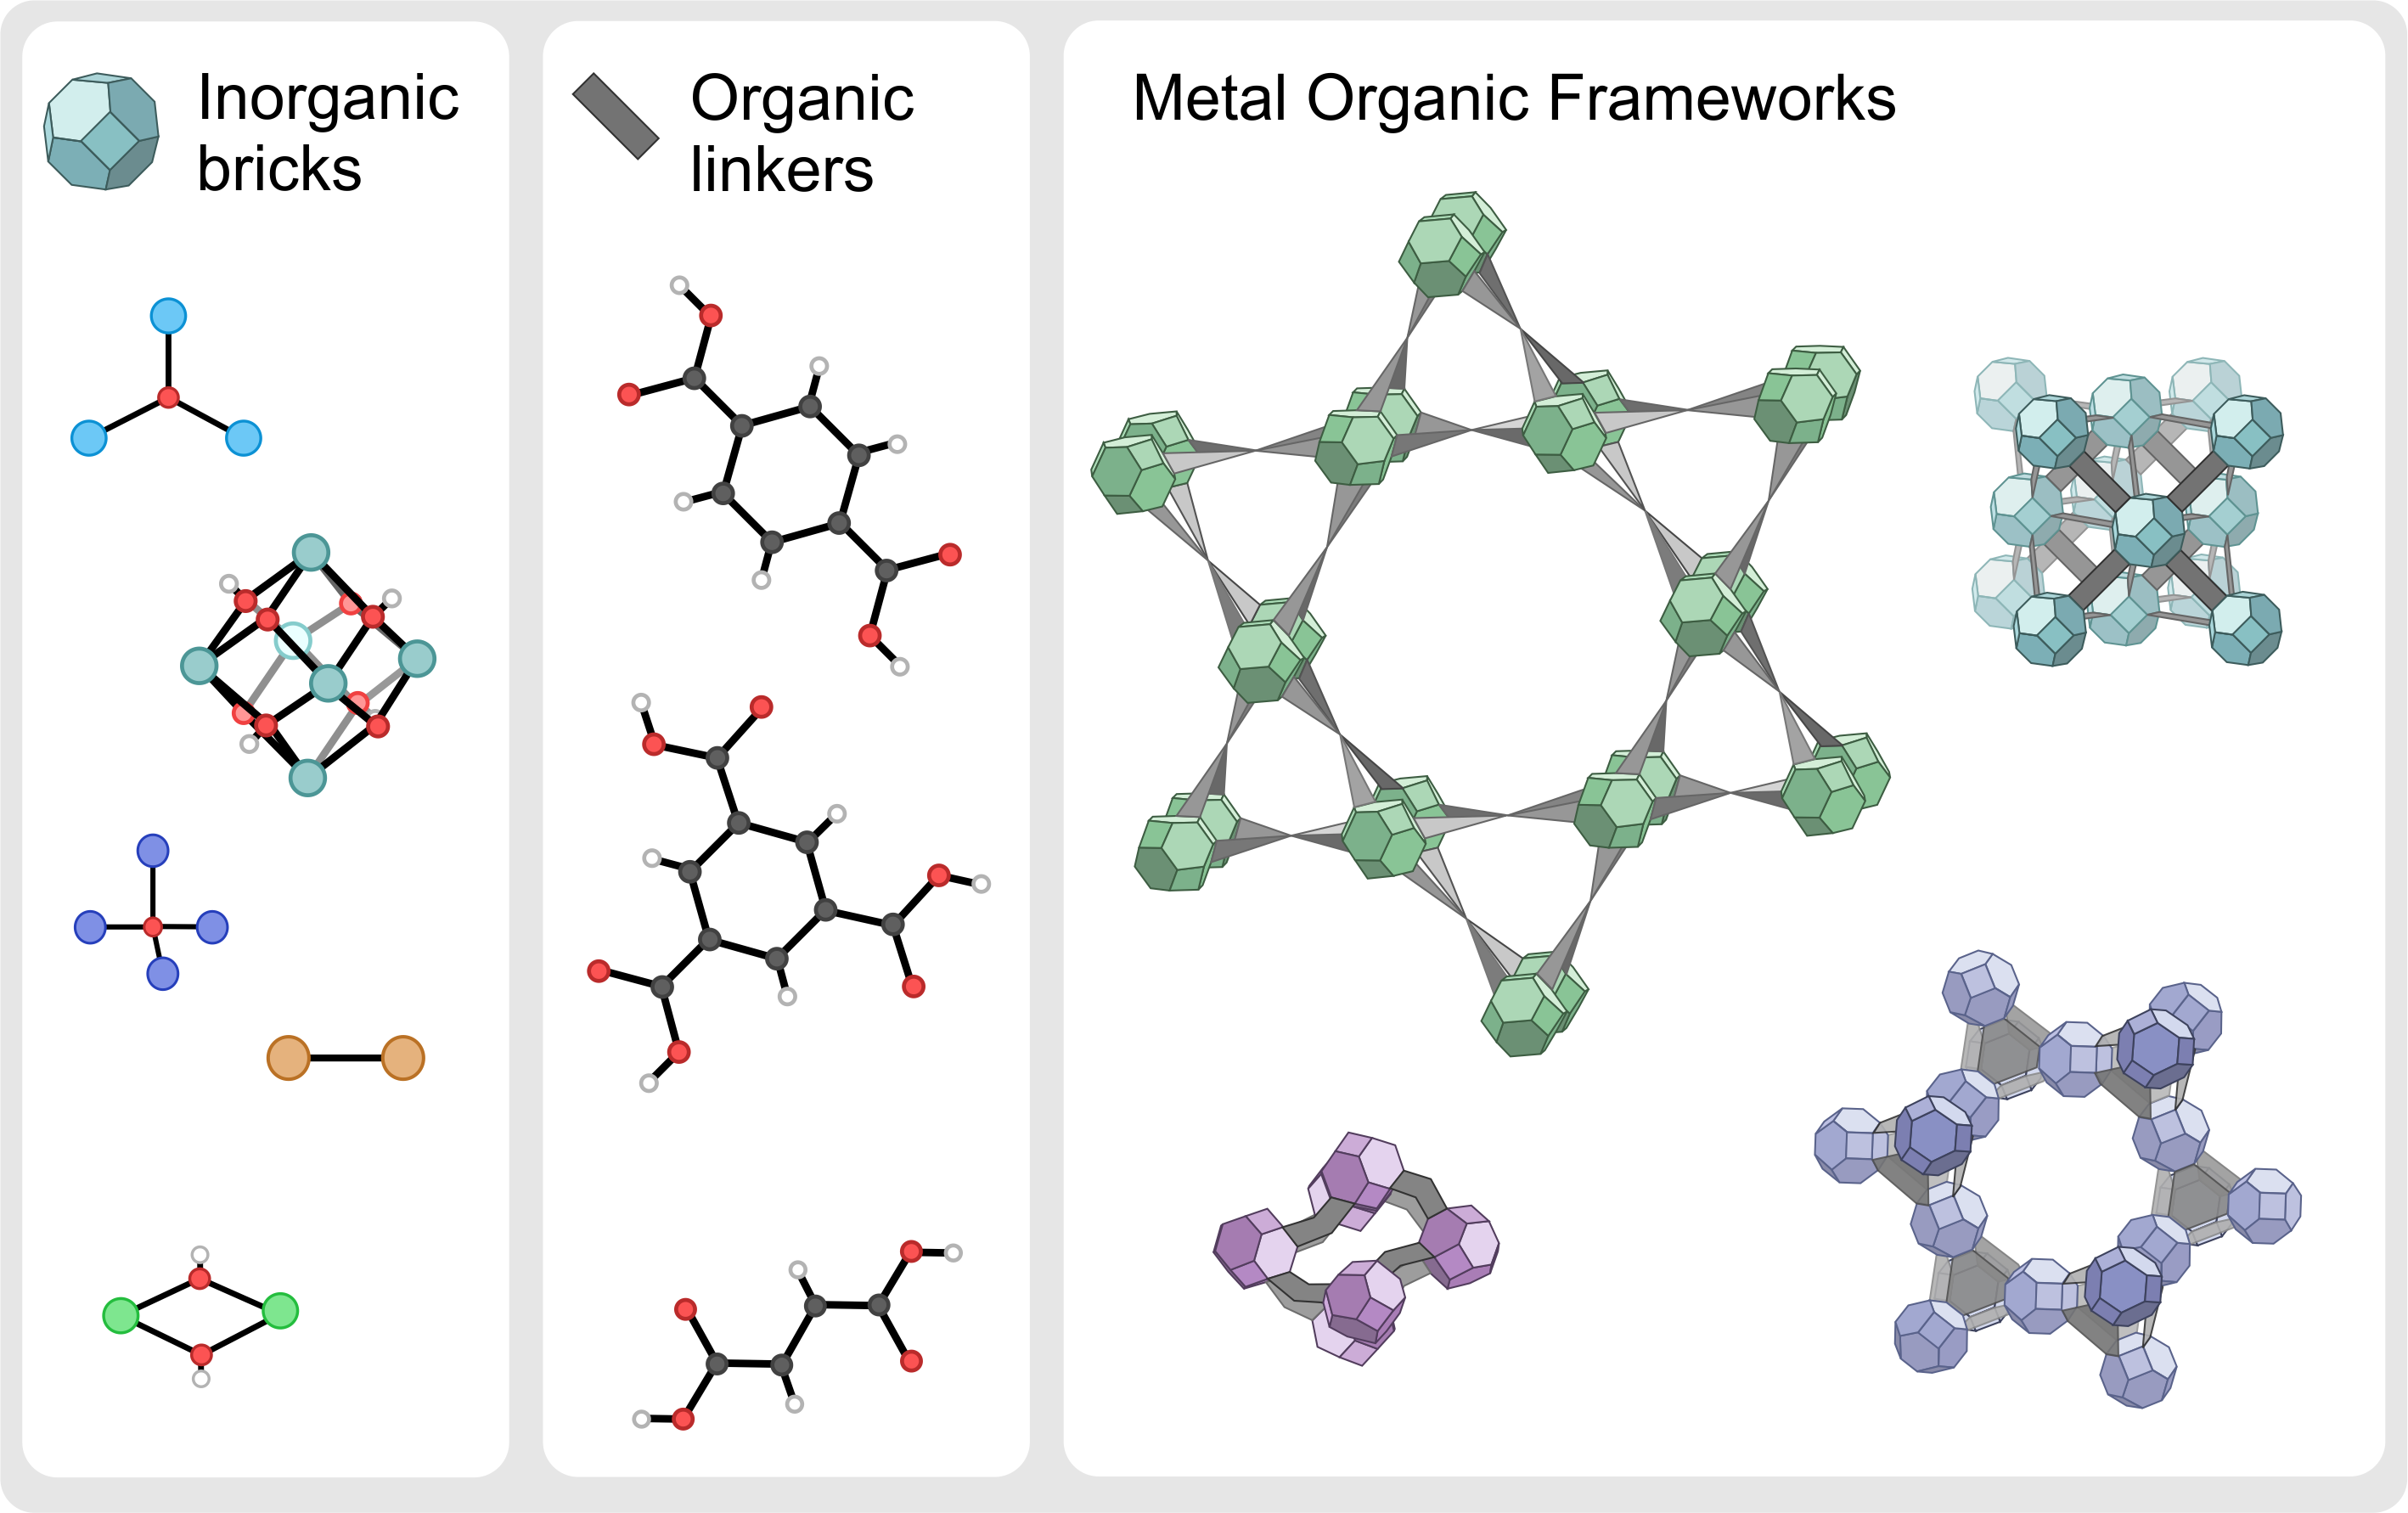
\includegraphics[width=1.0\textwidth]{MOFs}
	\caption{Schematic representation of the building block design in Metal-Organic Frameworks (MOFs). Left panel: some examples of inorganic bricks; middle panel: some examples of organic linkers; right panel: some MOFs with different topologies, pore size and shape}
	\label{fig:MOFs}
\end{figure}

\section{Metal Organic Frameworks}
MOFs are one of the most intriguing class of materials of current science. These materials, first called 'porous coordination polymers' (PCPs) were discovered in the late 50's, but only at the end of the past century with the works of Robson\cite{batten1995two,hoskins1990design}, Kitagawa\cite{kitagawa1991synthesis, kitagawa1993synthesis}, Yaghi\cite{yaghi1995hydrothermal} and F\'{e}rey\cite{riou1998hybrid}, the scientific community started to understand their full potential. At first the main focus of MOF research was in the discovery of new structures. However, in the last few decades, the field has seen an incredible explosion in scientific and industrial interest, with new applications being continuously explored\cite{furukawa2013chemistry}. MOFs are hybrid nanoporous materials that are composed by metal or metal--oxo clusters connected by multitopic organic linkers, to form multidimensional porous structures. Compared to the already well--known zeolites, MOFs can be constructed without templating agents, with a far greater number of metals and with an exceptional structural diversity. In fact, their particular building block design (Fig. \ref{fig:MOFs}), that makes use of secondary building units (SBUs), allows the creation of an almost infinite number of crystalline structures with different topology and chemical composition. The coordination bonds which lie at the basis of MOF structures are weaker than the inorganic zeolites. This on the one hand makes them less robust, but on the other allows facile structural modifications which are impossible to do on zeolites. In principle, the nature of the SBUs and their association can be finetuned\cite{stock2011synthesis}, allowing control of properties such as pore shape and size, functionalization, or surface area. The response to chemical and physical stimuli can this way be easily modulated \cite{zhou2014metal,zhou2012introduction}. 
One of the most intriguing concepts is the isoreticular synthesis, by which inorganic or organic SBUs can be replaced by topologically identical (or similar) building blocks. This way, starting from a given MOF precursor, whole families of MOF materials can be synthesized spanning a range of pore size and functionality. For instance, the pore size can be significantly increased up to the mesoporous range by using longer isoreticular linkers, such as in the IRMOF series, based on the MOF--5 precursor \cite{eddaoudi2002systematic}. 
%
%
\begin{figure}[htbp]
	\centering
 	\includegraphics[width=1.0\textwidth]{mof-applications}
	\caption{Schematic representation of some of the numerous MOF applications.}
	\label{fig:mof-applications}
\end{figure}
%
%
\npar
The tunability of MOF structures, along with their high crystallinity, metal content and porosity, are very appealing for application in different industrially relevant fields, such as catalysis, gas storage and separation, drug delivery or sensing, as displayed in Fig. \ref{fig:mof-applications}. At present moment, the main limitation for large scale application lies in the structural stability. More specific applications are being further explored, such as warfare agents decomposition, magnetic applications, or membrane separation \cite{furukawa2013chemistry}.
\npar
The study of MOFs has seen a continuous evolution in the past decades.
Following the nomenclature proposed by Kitagawa, we can differentiate between three generations of MOFs\cite{kitagawa1998functional}. First generation MOFs are defined as having a guest--molecules supported pore system that collapses when these are evacuated. For this reason, this first generation of MOFs found very limited use for practical applications. Those of second generation are more robust and have permanent porosity, that is retained even in absence of guest molecules. These materials show high potential for catalysis and other applications and are the main object of this dissertation. Finally, third generation MOFs are characterized by flexible pores that can reversibly change shape with the presence of guest molecules, or upon certain stimuli, such as temperature or pressure. Matsuka \textit{et al.}\cite{matsuda2004guest} identified five types of response mechanisms in MOFs, denoted as shrinking, expanding, reshaping, swelling and gate opening or closing. A perspective on the types of stimuli that can induce responsive in MOFs has been reported in the work of Coudert \cite{coudert2015responsive}.

\subsection*{Defects and active sites}
MOFs are crystalline materials that possess structural disorder, such as vacancies. If at first this was seen as a drawback, limiting stability, it has been accepted that they can play a key role in the performance of the material. Defect--containing MOFs and defect engineering have become an active field in MOF research, representing an additional way to finetune and enhance the material properties. 
Following the classification proposed by Sholl \textit{et al.} \cite{sholl2015defects}, defective sites in MOFs can be either point vacancies (such as missing linkers or clusters) or extended ones. Fang \textit{et al.} \cite{fang2015defect} further divided extended defects into dislocations, planar defects, and micro-- and mesoscale volume defects. 
\npar
At low defect concentration, a random distribution of isolated point defects can be found, whereas at higher concentrations clustering could occur\cite{cliffe2014correlated}, if the presence of a vacancy is influenced by other vacancies in proximity. The complexity arising from structural disorder makes the study of defects a current challenge in MOF research. In order to control their effect on certain properties, it is important to have precise information on their location, type and dispersion. Common experimental strategies for the characterization of defects in MOFs involve electron and fluorescence microscopy, Raman, infrared and X-ray spectroscopy, power and single--crystal X-ray diffraction\cite{fang2015defect}. Molecular modeling provides an important tool to obtain atomic scale resolution on the defect sites and understand how they impact specific properties.
\npar
Particularly for catalysis and adsorption, vacancies in the material lead to two main effects: 1) an increase in porosity and mass transport, and 2) the presence of undercoordinated metal atoms, introducing highly desired Lewis acid sites. 
%\subsection*{MOFs as single site catalysts}
In this sense, provided the structures are stable at reaction conditions (i.e. no leaking is observed), 
MOFs are true single--site heterogeneous catalysts, that contain well--defined active sites which are inherent part of the framework\cite{yang2019catalysis}. According to the classification proposed by Rogge \textit{et al.}, we can distinguish between three types of single--site catalysts in nanoporous materials, in which active sites for catalysis can arise from coordinatively unsaturated metals (type I), metal atoms embedded in porphyrin--based ligands (type II) or reactive functional groups (type III). Coordinatively unsaturated metal sites can present in the framework such as in HKUST--1\cite{chui1999chemically}, or can be introduced by intentional creation of defects, such as in the stable UiO--66 MOF \cite{vandichel2015active}. Another procedure that can lead to open metal sites without generating vacancies is the dehydration upon thermal treatment. To date, a plethora of MOFs have been synthesized possessing open metal sites. Their Lewis acidity can further be tuned by functionalization of linkers and bricks. This way, it is in principle possible to engineer a material for a target catalytic application.

\begin{figure}[!htbp]
	\centering
 	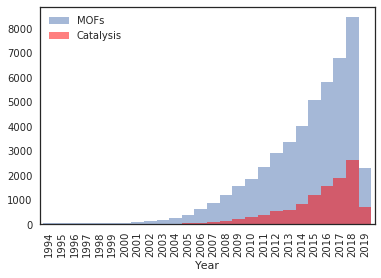
\includegraphics[width=0.8\textwidth]{citation_report}
	\caption{Number of publications on MOFs and catalysis in MOFs in years 1985-2018, showing the importance of catalysis in MOFs as indicated by Web of Science}
	\label{fig:citation_report}
\end{figure}
%
\subsection*{Post--synthetic modification}
When it is not possible to introduce functionalities with direct synthesis, post--synthetic modification (PSM) \cite{wang2009postsynthetic, cohen2011postsynthetic} has become a well established procedure that allows the preparation of MOF materials with specific chemical composition. Via this technique, it is possible to modify the crystal after the synthesis, allowing to finetune the properties of the material. Moreover, multi--functional sites can be integrated at the same time in the crystals \cite{li2016applications}. PSM strategies include encapsulation of guest molecules or nanoparticles in the pores, modifications of the linkers without breaking the metal--ligand bond, or post synthetic exchange (PSE) of linkers and metals, where building blocks are dynamically exchanged. PSE can also involve terminal ligands, or modulators, that do not contribute in connecting different bricks. This way, building blocks can be exchanged, but also eliminated to create vacancies, provided the material retains its crystallinity. For this reason, PSM has been used as an efficient strategy to introduce defective sites in MOFs. As one may expect, sufficient structural stability under the PSM conditions is a necessary prerequisite in order to apply PSM techniques \cite{garibay2010isoreticular}.
%
\subsection*{Stability}
In general, to function at operating conditions and to withstand modifications, materials need to retain their mechanical, chemical and thermal stability at those conditions. For instance, mechanical stability is needed when compressing MOF in pellets or other shapes for industrial processes\cite{chapman2009pressure}. Catalysis often also requires thermal stability, as the materials must be able to resist harsher conditions for certain processes such as in petrochemistry. Finally, chemical stability is crucial for many applications, such as drug delivery, molecular separation, or catalysis\cite{horcajada2010porous}. 
\npar
Unfortunately, the M--L coordination bond that makes MOFs so tunable is also regarded as one of their main drawbacks\cite{keskin2010can, canivet2014water, kizzie2011effect}, as it is responsible for the lower structural stability when compared to already established nanoporous catalysts such as zeolites. 
%For this reason, MOF research has focused on the development of stable materials. 
For example, the first synthesized MOFs such as \ce{Cu2+} trimesate HKUST-1, or MOF-5, composed by \ce{Zn2+} clusters and BDC linkers were degraded by water even at mild conditions\cite{greathouse2006interaction, low2009virtual, kaye2007impact, decoste2013effect}. Moreover, mechanical, thermal and chemical stabilities can further decrease in the presence of defects. Very few MOFs show stability towards water and at different pH conditions\cite{leus2016systematic}, such as Zr--based MOFs. 

\subsection*{Zr--based MOFs}
%%
\begin{figure}[!htbp]
	\centering
 	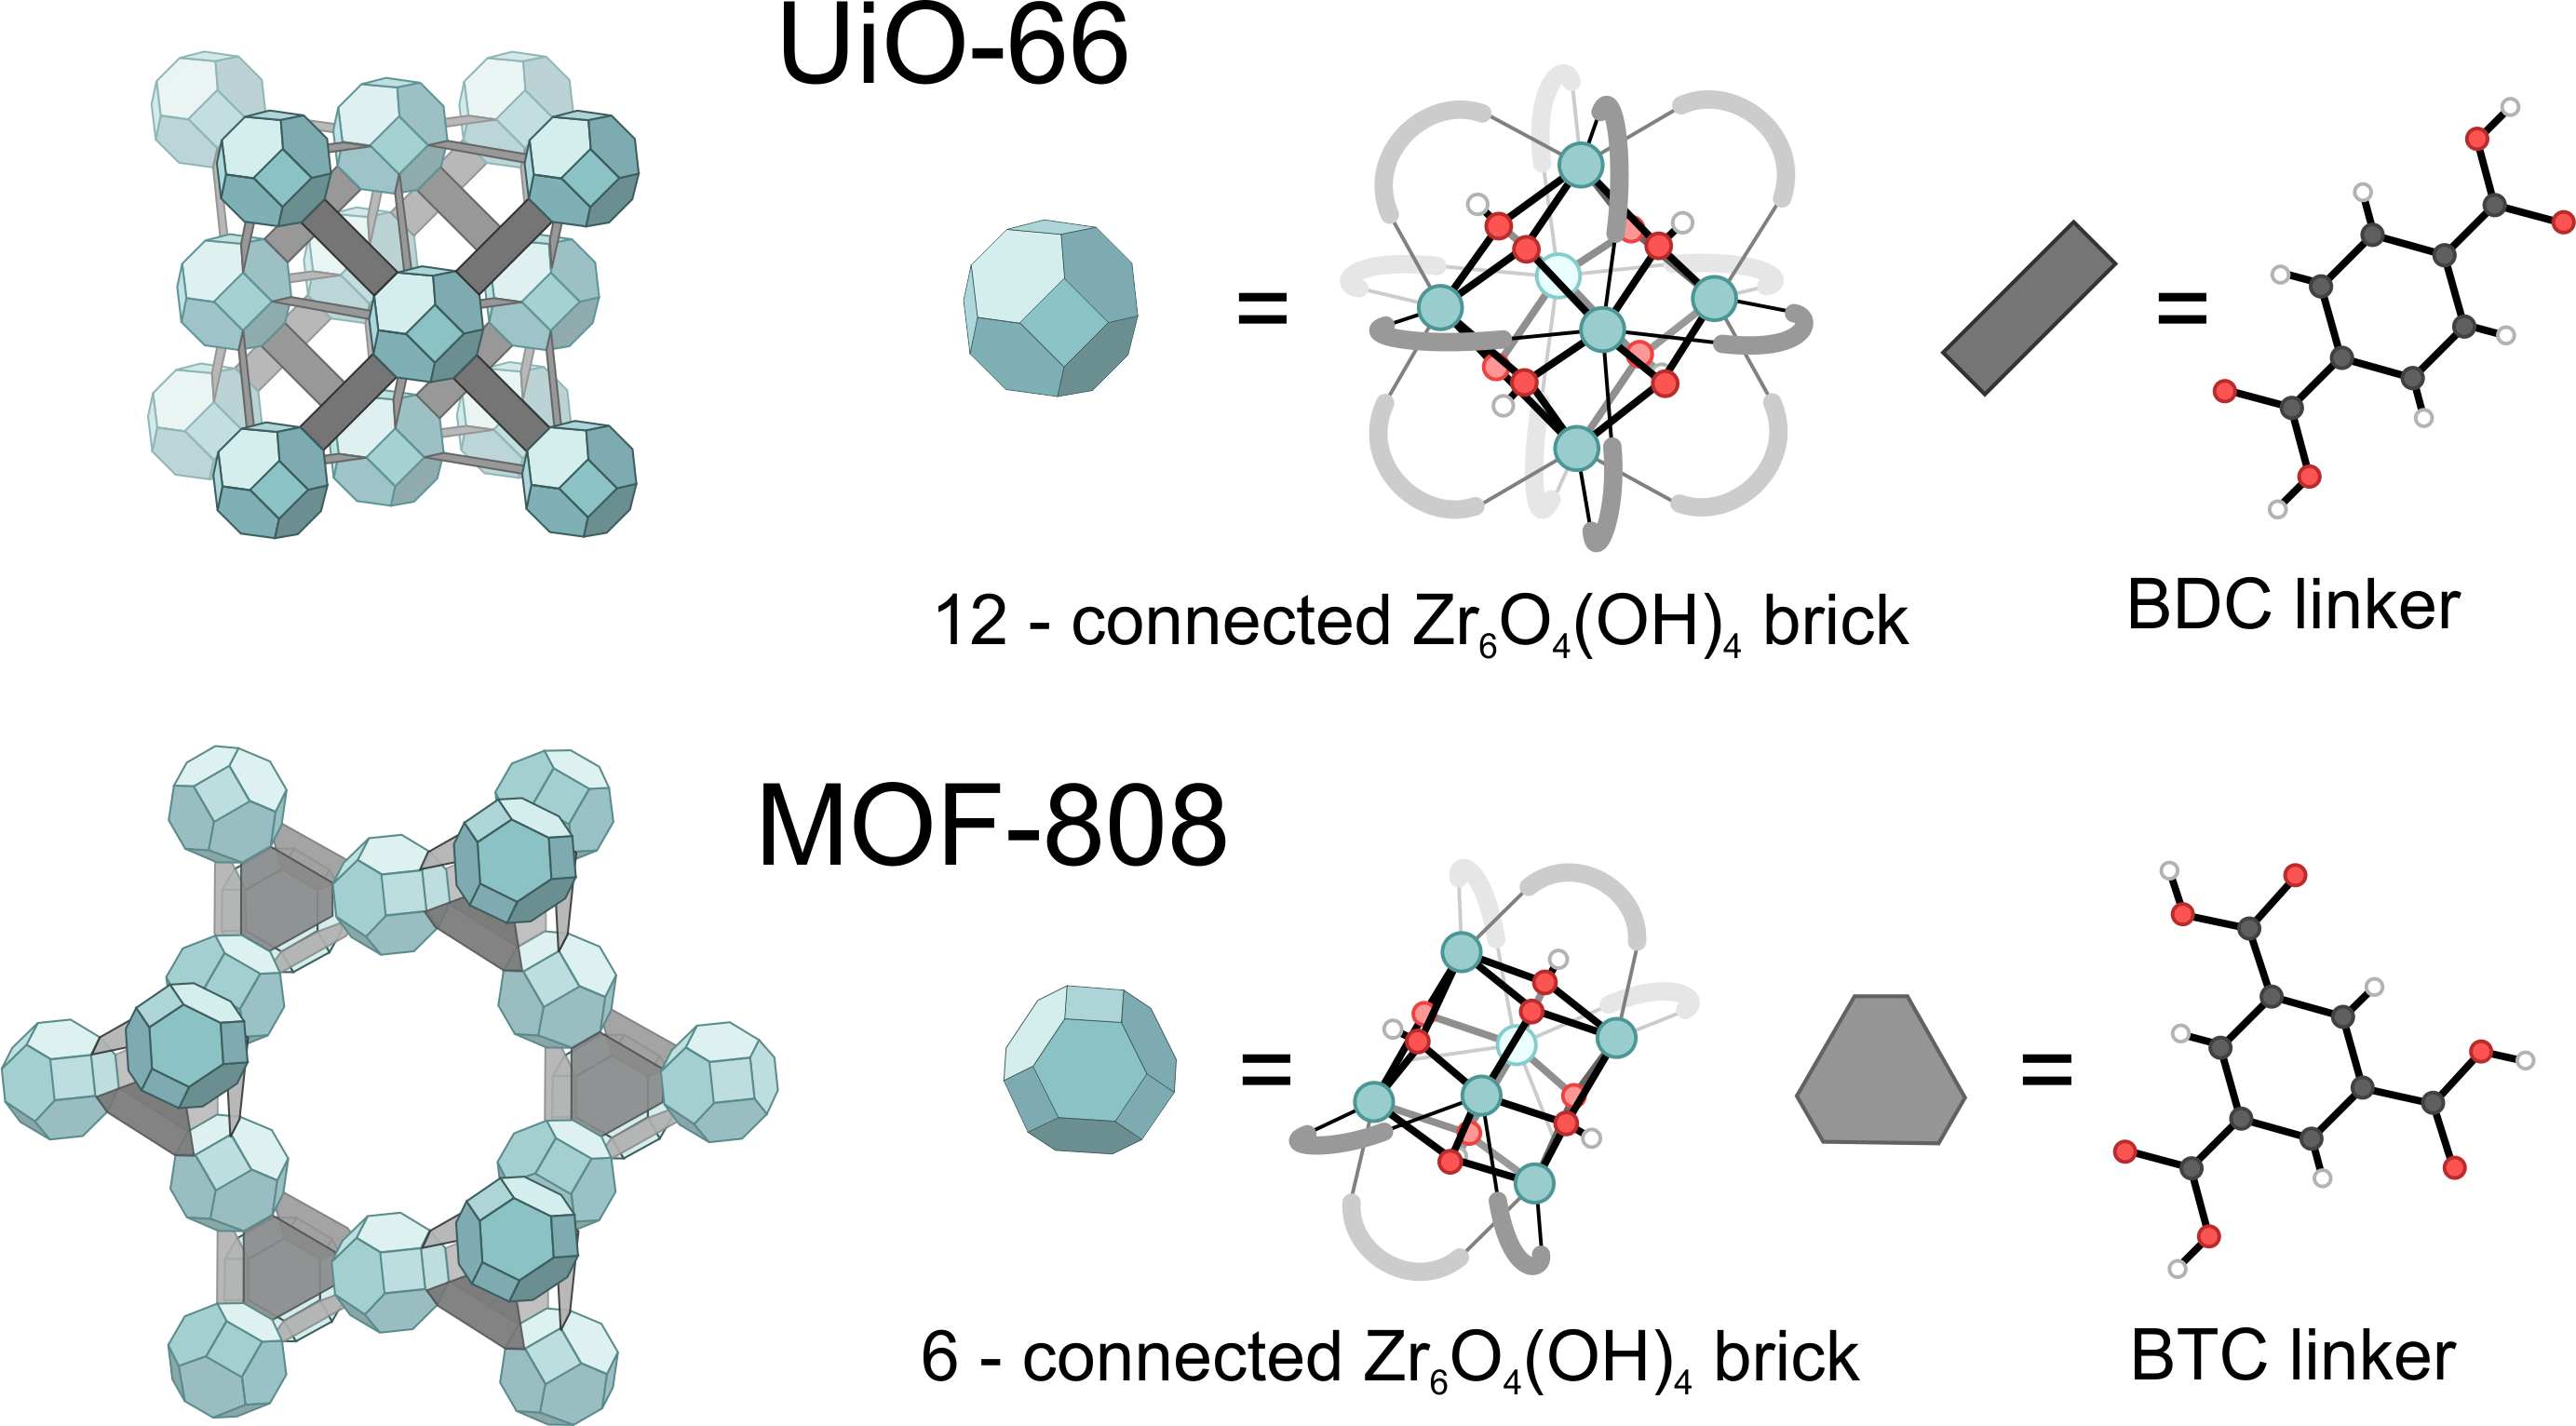
\includegraphics[width=1.0\textwidth]{Zr-MOFs}
	\caption{Structure of UiO--66 (top) and MOF--808 (bottom), the two Zr--MOFs investigated in this work of thesis.}
	\label{fig:Zr-MOFs}
\end{figure}
%%
Recently, a class of outstandingly robust MOFs have been synthesized \cite{furukawa2014water}. Zr--based MOFs\cite{bai2016zr} which exploit the robustness of the Zr--O bond, show an unprecedented stability and are at present time one of the most studied classes of MOFs. Moreover, zirconium is an ubiquitous metal that is present in biological systems and has low toxicity, as well as limited cost. This makes these materials particularly promising for applications in catalysis, gas sorption, and drug delivery. An overview of the plethora of possible structures that can be synthesized with different inorganic SBUs can be found in a recent review by Bai \textit{et al.} \cite{bai2016zr}.
\npar
The vast majority of these materials is characterized by Zr(IV) atoms in a high coordination state (Fig. \ref{fig:Zr-MOFs}), which interact strongly with the oxygens of carboxylate linkers of various topology. These MOFs are characterized by a \ce{Zr6O4(OH)4} cluster in which each of the 6 zirconium atoms is connected to 4 oxygen atoms (two $\mu_3$--OH and two $\mu_3$--O), each of which is in turn connected to three zirconium atoms, forming a polyhedron. Each zirconium atom can form 4 other bonds with ligands, accommodating up to 24 metal--ligand bonds per cluster. Every zirconium atom can therefore form a total of 8 coordination bonds oriented in a square--antiprismatic geometry, yielding a rich range of possible structures that can be synthesized with connectivity ranging from 12, as in UiO--66\cite{cavka2008new}, to 6 which is found in MOF--808\cite{furukawa2014water} (see Fig. \ref{fig:Zr-MOFs}). The dual Lewis acid/base nature of the Zr--carboxylate bonds, along with the high metal oxidation state, gives rise to strong interactions between the SBUs, thus allowing processes such as PSM without compromising the stability of the structures. The high degree of connectivity between inorganic and organic SBUs lies at the origin of the high structural stability found in Zr--based MOFs\cite{bai2016zr, leus2016systematic}. Open metal sites in these materials can be present if the brick connectivity is lower than 12. This can be an inherent property of the structure, such as in the 8--fold connected NU--1000 \cite{mondloch2013vapor}, or can be induced by introduction of structural defects. Zirconium atoms that remain undercoordinated are Lewis acid sites where reactants can adsorb and that can function as catalytic centers.

\subsection*{UiO--66}
The first material belonging to this class of Zr--based MOFs is the Zr--therephtalate based UiO--66, and was first synthesized at the Universiteit i Oslo (UiO) by Lillerud and coworkers\cite{cavka2008new}. The UiO-66 material, shown in Fig. \ref{fig:Zr-MOFs}, is one of the most studied MOFs thus far and was an inspiration of other MOFs within this family. UiO--66 is characterized by an extremely high connectivity that gives rise to an exceptional structural stability. In this material, each \ce{Zr6} SBU is connected to 12 therephthalate (or benzenedicarboxylate (BDC)) linkers forming a cubic close packed structure with a space group F\={m}3m, No. 225. In this structure there are two different cavities of octahedral and tetrahedral shape, with window sizes of 10 \AA\ and 25 \AA, respectively. Each octahedral cage shares triangular windows with eight tetrahedral cages. 
This results in an extremely robust material which is stable up to 648 K and in a broad range of protic and aprotic solvents and pH conditions. Moreover, the \ce{Zr6O4(OH)4} bricks can be reversibly dehydrated upon thermal treatment at temperatures between 523 and 573 K. Up to two water molecules can be formed this way, yielding a \ce{Zr6O6} brick, where the zirconium atoms have a coordination of 7\cite{valenzano2011disclosing}. Lowering of zirconium coordination by dehydration can be a strategy to create open metal sites, along with the creation of defects.
\npar
A whole family of isoreticular MOFs can be derived from UiO--66 by using linkers of different size, spanning from fumaric acid\cite{wissmann2012modulated} up to terphenyldicarboxylic acid\cite{schaate2011modulated}, allowing to significantly tune pore size and surface area. Interpenetrated MOFs with UiO--66 topology have been also reported if longer linkers are used\cite{schaate2011porous}, with a decrease in surface area. Moreover, different functional groups can be appended to the phenyl rings, such as bromo, amino, nitro, or naphthalene. Garibay and Cohen showed that UiO--66--\ce{NH2} can be further modified to yield new functionalized frameworks \cite{garibay2010isoreticular}. Also the inorganic SBUs can be modified, for instance introducing titanium or hafnium\cite{kim2012postsynthetic}. Moreover, PSM can lead to creation of defects and open metal sites, as will be shown in \textbf{PAPER IV}. The exceptional thermal and chemical stability of UiO--66, along with its high connectivity, allows all these modifications of the structure, and for this reason, this material is often considered as a perfect MOF archetype, where new techniques can be tested. 

\begin{figure}[!htbp]
	\centering
 	\includegraphics[width=1.0\textwidth]{defectiveuio}
	\caption{Representation of the UiO--66 material with missing linkers and clusters displayed in red. In this dissertation, we mainly focus on missing linkers.}
	\label{fig:defectiveuio}
\end{figure}

\subsubsection*{Defects on UiO-66}
%chap 11 of book from Garcia
%The perfect crystalline UiO--66 structure, where every zirconium atom is 8--fold coordinated, does not possess open metal sites for catalysis. 
The high connectivity of the UiO--66 material allows the presence of structural vacancies. It has been generally accepted that the material can contain defects in the form of missing linkers or clusters (Fig. \ref{fig:defectiveuio}). These defects naturally originate during synthesis, as shown by experimental results, such as symmetry--forbidden reflections in the PXRD pattern, metal--linker ratio obtained by thermogravimetric analysis (TGA), higher than expected surface area, appearance of O--H stretching bands in the FTIR spectrum etc. \cite{shearer2014tuned, valenzano2011disclosing}. Moreover, it was later discovered that the number of defective sites can easily be tuned by adapting the synthesis conditions, such as temperature and type of modulator\cite{wu2013unusual, shearer2016defect}. 
\npar
Defects can influence the material properties to a large extent. The beneficial role of defects in UiO--66 has been explored in many applications such as gas storage and separation\cite{wu2013unusual, ren2014modulated}, sensing\cite{stassen2016towards}, drug delivery\cite{cunha2013rationale} and catalysis\cite{vermoortele2013synthesis, rogge2017metal}. The physical properties of defective UiO--66 differ according to the number of defects and their location, as has been extensively studied both theoretically and experimentally \cite{rogge2016thermodynamic, devos2017missing, cliffe2014correlated, borges2016proton}. A decrease in the connectivity in the structure will naturally lead to a decrease in stability of the material. However, the extremely high connectivity of UiO--66 allows the presence of numerous missing linkers or cluster without loss of crystallinity. In this context, Rogge \textit{et al}. investigated the influence of all possible configurations of one to two linker vacancies on the stability of UiO-66. The equilibrium volume is not affected by such vacancies, however properties such as bulk modulus and loss--of--crystallinity pressure, which in turn influence the stability, are affected by the number and configuration of missing linkers \cite{rogge2016thermodynamic}. 
De Vos \textit{et al}.\cite{devos2017missing} investigated the electronic properties for all possible configuration of defective UiO--66 with up to three missing linkers, showing that some configurations are energetically more stable than others, and that the number and position of missing linkers affect the band gap of the material. From these studies performed on small unit cells, it is already clear that the number of possible defective configurations can be extremely high, and it is still unclear to what extent such point defects are disordered in the material. A regular distribution of point defects that involve missing clusters can lead to different phases in the material, from fcu (non-defective), to bcu (missing linkers with open channels), reo (missing clusters) to scu (missing linkers and missing clusters). Missing clusters could in principle increase the catalytic activity of the material more than missing linkers due to the larger pore size. Recently, Cliffe \textit{et al}. \cite{cliffe2014correlated} showed in a combined theoretical-experimental work that missing clusters on UiO-66(Hf) were correlated and formed nanodomains in the material, characterized by a reo phase. These reports shed light into the complexity of modeling disorder in nanoporous materials. 

\subsubsection*{Active sites for catalysis in UiO--66}
One of the breakthroughs of MOF research was the discovery that UiO--66 could contain a high number of open metal sites. As reported earlier, active sites for catalysis in UiO--66 and other Zr--MOFs are present when the zirconium connectivity is decreased from its equilibrium value of 8.
\npar
%active sites by defects
A first way to obtain coordinatively unsaturated zirconium sites is by creation of defects, in the form of missing linkers or clusters. The inherent vacancies in UiO--66 bring unsaturated zirconium Lewis acid sites\cite{wu2013unusual, shearer2014tuned, vermoortele2013synthesis, vandichel2015active, liu2016probing} and at the same time enhance the accessibility of the reactants to the active sites as the pore volume increases. The synthesis of defective UiO--66 can be tuned via modulators such as formic acid or trifluoroacetic acid (TFA), that are competing with BDC linkers in binding to the inorganic SBU. 
Vermoortele \textit{et al}. first showed in a dual computational--experimental study that the Lewis catalyzed cyclization of citronellal requires missing linkers\cite{vermoortele2012electronic}. For Meerwein reduction, another Lewis catalyzed reaction, the catalytic activity of UiO--66 could be significantly increased by making use of TFA, that introduced a large number of linker vacancies. Additionally, the non-modulated material that contained only a small number of defects showed nearly no catalytic activity\cite{vermoortele2013synthesis}. Such relationship between catalytic activity and amount of defects has been reported for different Lewis catalyzed reactions giving clear evidence that the catalytic centers are located on the defective sites\cite{vermoortele2012electronic, vermoortele2013synthesis}. 
\npar
The molecular characterization of the defective sites on UiO--66 has been an ongoing research interest in MOF literature. Particular focus has been given on the species adsorbed on the defective site and on the coordination environment of zirconium. Lillerud and coworkers \cite{oien2014detailed} reported that when linker vacancies were present, XRD characterization of the material showed two type of Zr--bonded oxygen atoms. The first type was BDC oxygen, and the other was associated to water species coordinated to the zirconium on the defect site. Later from SXRD measurements, the group of Yaghi \cite{trickett2015definitive} proposed that the two Zr--bonded oxygens belonged to physisorbed water molecules and that the charge compensating species was a hydroxyl group. However, following reports did not confirm such configuration. 
\npar
Molecular simulations were essential to shed light into the detailed molecular structure of the defective brick. Ling and Slater \cite{ling2016dynamic} performed MD simulations starting from the configuration proposed by Yaghi and showed a progressive stabilization towards another structure where the two adjacent zirconium atoms were coordinated to a physisorbed water molecule and a hydroxyl group, as shown in Fig. \ref{fig:bronsted-lewis-uio}. These sites have been confirmed by a comprehensive computational study of different adsorption possibilities of up to three water molecules on defective UiO--66 performed by Vandichel \textit{et al}. \cite{vandichel2016water} and by simulations performed in this work of thesis.
Such water and hydroxy species are strongly interacting with the zirconium atoms and are sources of Br\o{}nsted sites, as indicated in Fig. \ref{fig:bronsted-lewis-uio}. It was remarkable to discover that some catalytic processes are not catalyzed by undercoordinated Lewis acid sites, but need also Br\o{}nsted sites arising from defect--coordinating species, as will be shown in \textbf{PAPER I}. Apart from the interactions of water with the active sites, they may also have a strong influence on the proton conductivity of the material. Serre and coworkers reported that a hydrogen bonded network that spans the octahedral and tetrahedral cages is responsible for the high proton conductivity showed by UiO-66 at high temperatures \cite{borges2016proton}. Kitagawa \textit{et al.} showed the positive role of defects in proton conductivity in the UiO-66 material, as defective sites provide both larger pores and zirconium undercoordinated sites where water species are adsorbed and can function as proton donors \cite{taylor2015defect}. Farha and coworkers identified three types of acidic protons in the material by means of potentiometric titration: $\mu_{3}$--OH belonging to the inorganic SBU, and two arising from subsequent deprotonation of the physisorbed water and hydroxyl group on the defective site. They made use of the acidic protons belonging to physisorbed water for a quantification of defects in the material \cite{klet2016evaluation}. The mechanism associated to the change in topology of the hydroxyl groups on the inorganic SBU has been investigated by Yang \textit{et al}.\cite{yang2016tuning}. The interaction between defect--coordinating water molecules and zirconium atoms is strong, and UiO--66 can be partially hydrolized\cite{decoste2013stability} while retaining its stability, as will be further discussed in this dissertation.
\npar
The defect--coordinating species can be removed by thermal activation at T $>$423 K (more information on this process is given in \textbf{PAPER I}). The more loosely bonded physisorbed water is the first to leave the defective site, followed by the chemisorbed water. The dehydrated active site obtained this way is missing a $\mu_{3}$--OH proton and has two 7--fold coordinated zirconium open metal sites as shown in Fig. \ref{fig:bronsted-lewis-uio}. 
\npar
%active sites by dehydration
The second activation process by which open metal sites can be created on UiO--66 is the reversible dehydration of the \ce{Zr6O4(OH)4} cornestone to obtain \ce{Zr6O6} by removal of up to two water molecules performed at a temperature range between 523 and 573 K \cite{valenzano2011disclosing}. In this case also 7-fold coordinated zirconium atoms are created and may take the role as Lewis active sites, however the increase in pore size due to linker vacancies does not occur, and the active sites are less accessible than in the defective material. For instance for the citronellal cyclization \cite{vermoortele2012electronic}, in absence of defects, linkers should still be partially decoordinated to make space for the reactants to adsorb on the zirconium atoms.

%The presence of these species give a dual Bronsted--Lewis catalytic nature to UiO--66.
%The electroneutrality of the structure makes it so that at least one negatively charged species has to be coordinated to the inorganic SBU. 
\begin{figure}[!htbp]
	\centering
 	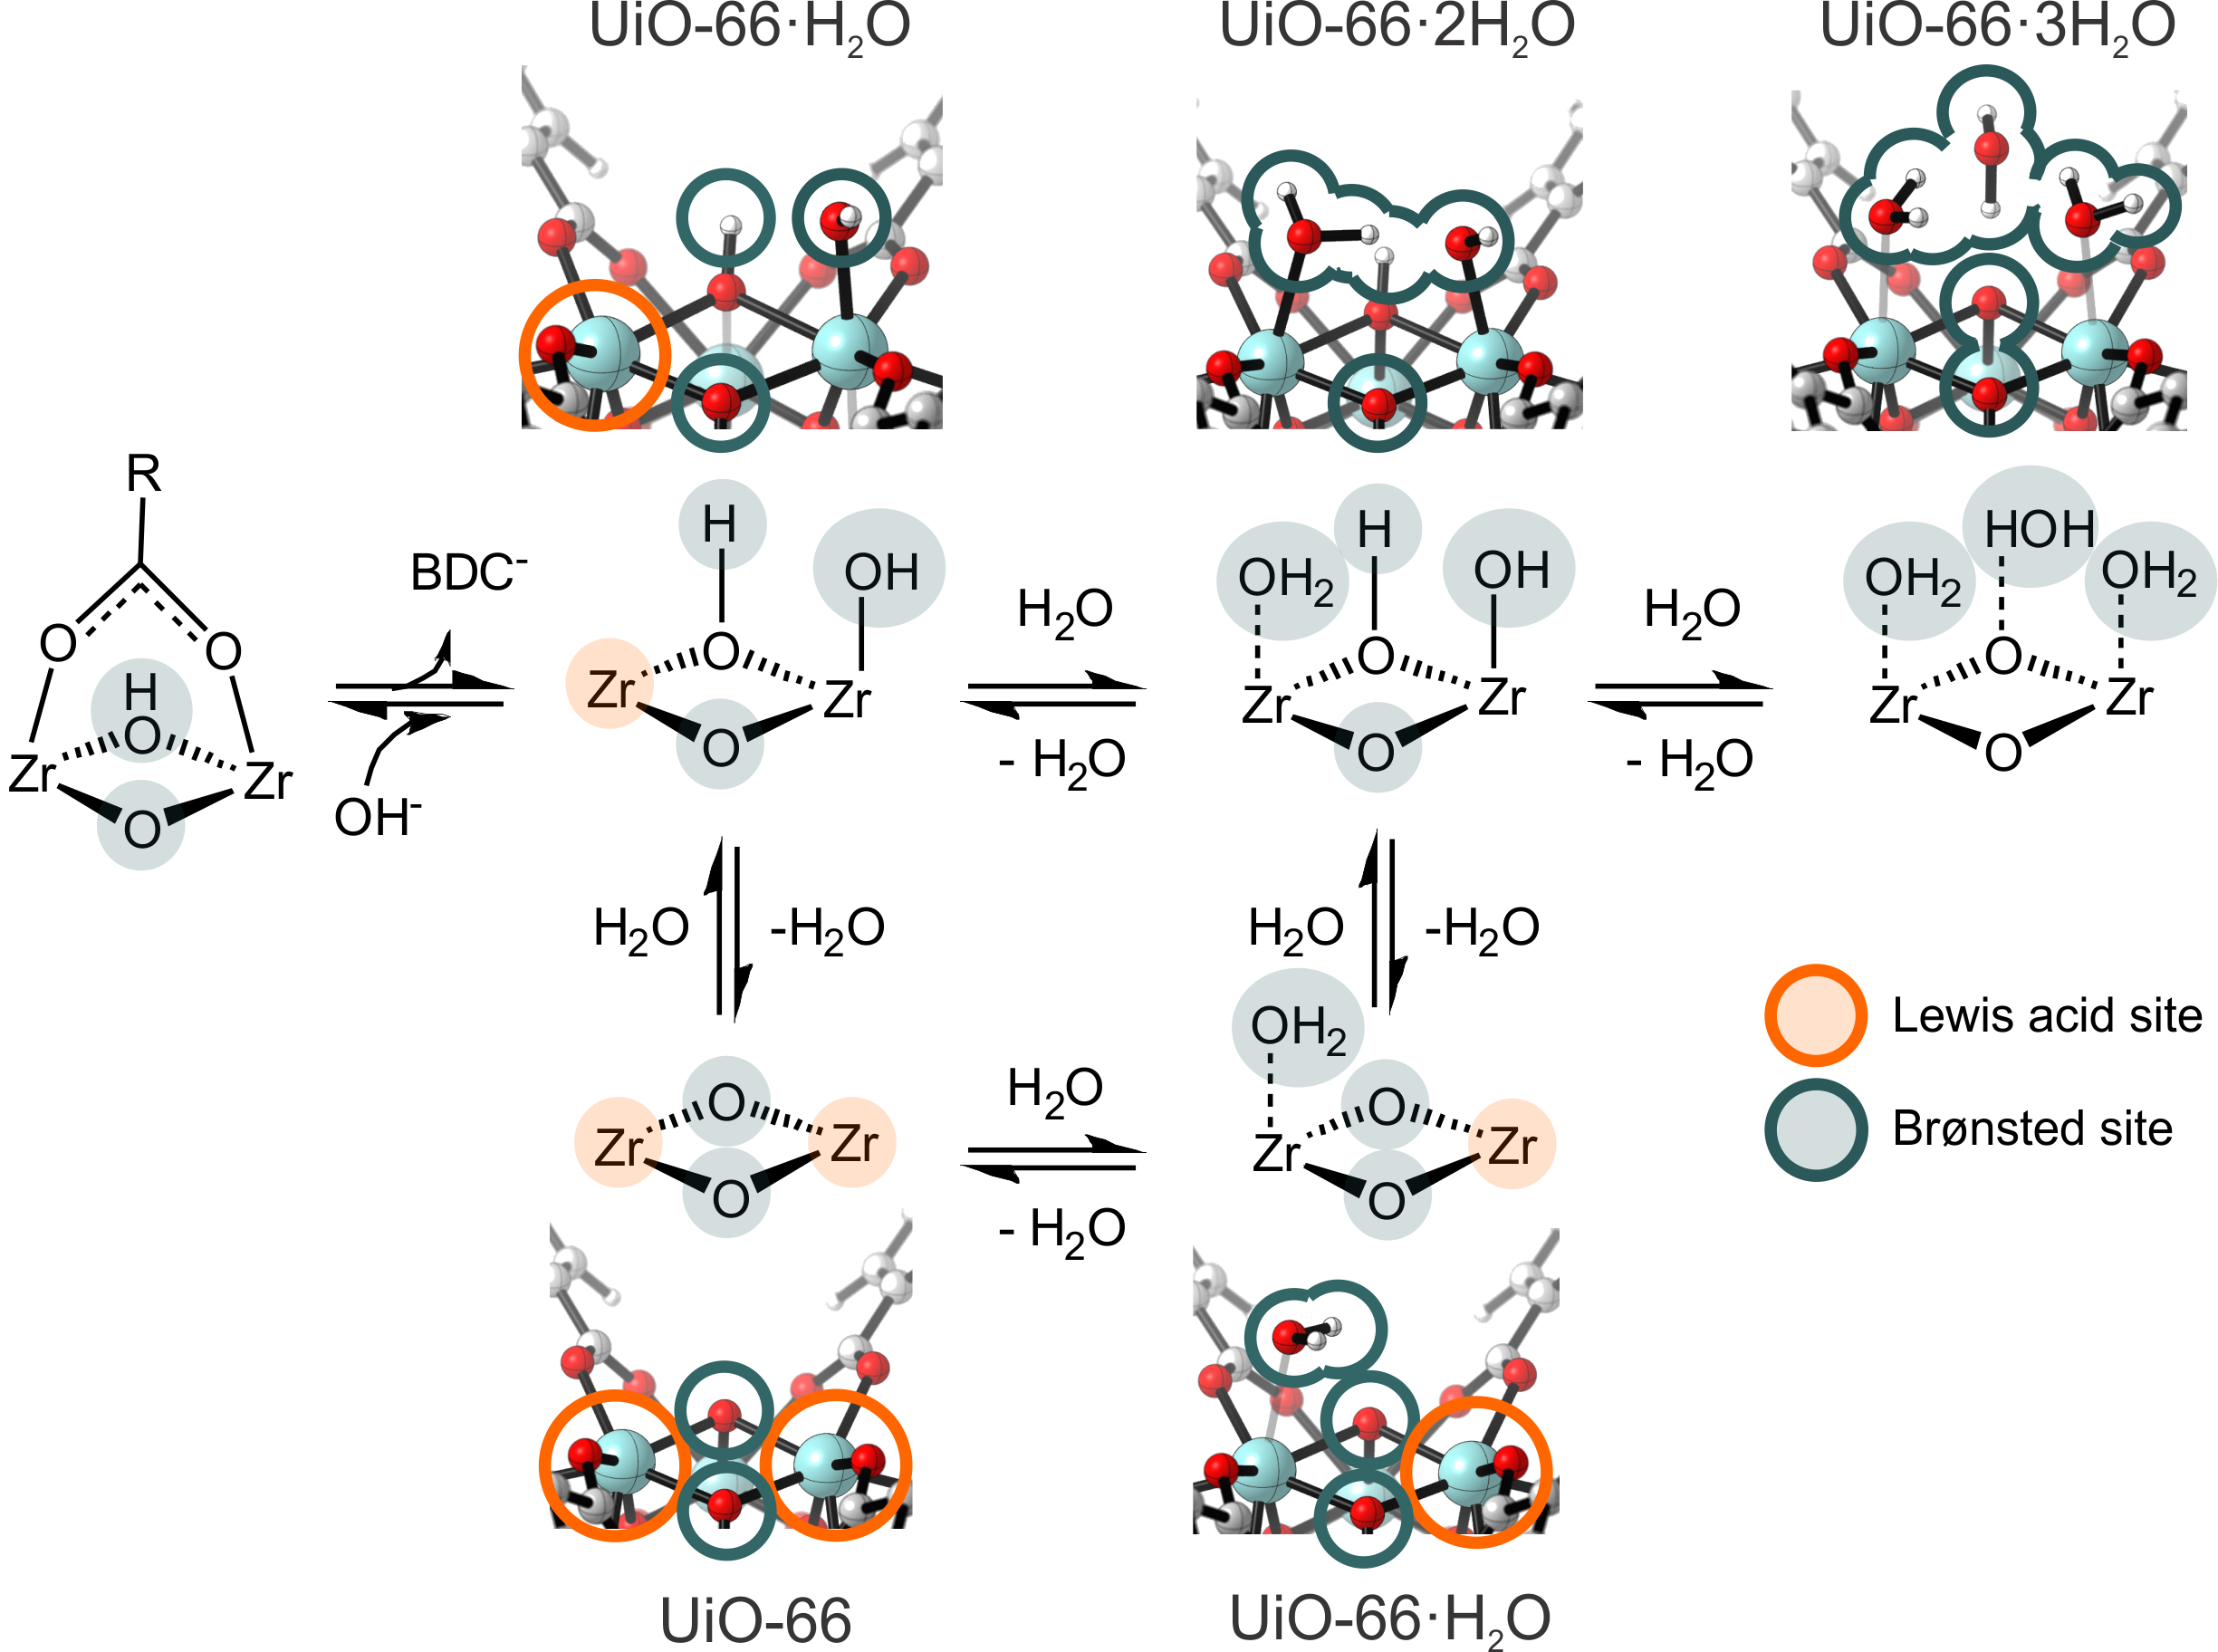
\includegraphics[width=1.0\textwidth]{bronsted-lewis-uio}
	\caption{Lewis and Br\o{}nsted sites that are created when a linker is removed from the UiO--66 zirconium brick, with different number of coordinated water molecules.}
	\label{fig:bronsted-lewis-uio}
\end{figure}
\subsubsection*{Functionalization of UiO--66}
\td{add here reaction scheme?}
Reactions on UiO--66 can proceed exploiting purely the Lewis acidity of undercoordinated zirconium atoms, or can also make use of Br\o{}nsted sites located on the defect sites. The acidic and basic properties of such groups can be further influenced by linker functionalization \cite{kandiah2010synthesis, kandiah2010post, kim2012discovery}. Functionalization, which can be done via PSM, represents a strategy to further finetune the properties of the material. 
For instance, the presence of electron--donating substituents showed an increase in catalytic activity for jasminaldehyde condensation \cite{vermoortele2011amino}. A positive effect of electron--withdrawing group was found by the same authors for Lewis catalyzed citronellal cyclization \cite{vermoortele2012electronic}. The beneficial role of amino groups was reported as well by Timofeeva \textit{et al}. \cite{timofeeva2014effects} for acetylisation of benzaldehyde, as well as by Cirujano \textit{et al} \cite{cirujano2015zirconium, cirujano2015conversion} for esterification. The electron donating effect of amino groups would in principle lead to a decrease in the Lewis acidity of the defective zirconium atoms, lowering the reaction rate. Therefore, a change in mechanism in the presence of BDC--\ce{NH2} was hypothized. However, Hajek \textit{et al}. further studied aldol condensation in a computational work\cite{hajek2015mechanistic}, and reported a beneficial, but passive role of amino groups, which is further confirmed in \textbf{PAPER I} for Fischer esterification. 

\subsection*{Active sites on MOF--808}
\begin{figure}[!htbp]
%\vspace{-2cm}
	\centering
	\includegraphics[width=1.0\textwidth]{MOF-808-dehydration}
	\caption{Schematic representation of as synthesized and upon activation MOF-808 structures}
	\label{fig:MOF-808-dehydration}
\end{figure}
If active sites can be introduced on UiO--66 by linker/brick removal and dehydration, other less connected Zr--based MOFs contain inherent vacancies due to their topology. Materials such as NU--1000 and MOF--808, although less robust than UiO--66, possess a higher number of active sites and larger pores and for this reason they are regarded as promising heterogeneous catalysts. 
MOF--808, formed by the inorganic \ce{Zr6O4(OH)4} cornestone and trimesate (BTC) linkers, represent the least connected MOF in the Zr--MOF family \cite{furukawa2014water}, and its brick can be regarded as an extreme case of the defective UiO--66 (Fig. \ref{fig:MOF-808-dehydration}). 
MOF--808 is a promising catalyst that is still less studied than UiO--66, but has a lot of potential for possible applications. For instance, it shows a higher catalytic activity for certain Lewis catalyzed reactions, such as Meerwein-Ponndorf-Verley (MPV) reduction \cite{plessers2016zr, mautschke2018catalytic}. Moreover, MOF--808 represents the first evidence of a superacid in MOFs, showing superacidity after post--synthetic treatment with sulfuric acid \cite{jiang2014superacidity}.
\npar
The rigid BTC tritopic linkers stabilize the structure and yield exceptionally wide channels which are required for the diffusion of substrates. The octahedral crystals contain 6 BTC linkers per inorganic node and are characterized by a \textit{spn} topology. 
In the material, each zirconium atom is bonded to four oxygens from the inorganic brick and two oxygens from the BTC linkers. The other two bonds that are needed to reach the total coordination of 8 are provided by species present in solution that do not contribute to the framework connectivity. 
\npar
In the as--synthesized material (Fig. \ref{fig:MOF-808-dehydration}), the zirconium atoms are capped with the relative mobile formate modulator. The material at this stage does not contain catalytically active sites and must be activated by post--synthetic treatment. By hot filtration, the formate groups can be eliminated and replaced by solvent water and hydroxyl groups \cite{plessers2016zr, mautschke2018catalytic}. In the catalytically active material, each brick is connected to six BTC linkers, six water molecules and six hydroxyl groups, and possesses a high number of potential Br\o{}nsted sites. Klet \textit{et al}. reported the presence of four different types of protons in the material \cite{klet2016evaluation}, each yielding a different acidity. The acidity of these protons can influence reactions, and its characterization represent a current challenge. From this structure, Lewis acid sites can be created by thermal activation, similarly as in UiO--66. In this case, hydroxyl groups remain connected to the zirconium atoms and the material possesses both Lewis and Br\o{}nsted sites that can be used for reactions. Moreover, the hydroxyl groups could further be used as anchors to incorporate new features in the material. 

\section{Outline and goal of the thesis}
In this chapter, the main characteristics of MOFs, making them appealing for catalysis, have been introduced, as well as the main computational results illustrating the complementary role of molecular modeling in unraveling the material properties. 

\td{take from Julianna}
%by experimn. you cannot track
%dynamic behavior, therefore enhanced sampling
The work of this thesis aims at understanding the nature of the active sites in zirconium MOFs such as UiO--66 and MOF--808 by means of molecular modeling techniques. 
In particular we focus on the effect of functionalization and the influence of protic species adsorbed on the defective site. We extended this concept to provide a description at operating conditions of the defective sites and how the presence of solvent influences the behavior of the material for catalysis.\\


%Molecular modeling can give fundamental insight into the properties of MOFs, and at present time a plethora of different techniques are available for this purpose. 
%To model processes in MOFs, knowledge of both power and limitations of these methods and experimental insight into the scientific question are required to find the appropriate combination of techniques.\\
This PhD thesis is organized as follows:
\begin{itemize}
\item In Chapter 2, a condensed theoretical overview of current molecular modeling techniques within MOF research is given. Particular attention is drawn on how these techniques can be applied to obtain insight into structural and catalytic properties at operating conditions.
\item In Chapter 3, the main results of this PhD thesis are summarized. The links between theory and experiment are highlighted throughout the chapter. All results are the result of fruitful experimental and theoretical collaborations and have been published in international peer--reviewed journals. 
\item In Chapter 4, the main conclusions of this thesis work, as well as perspectives on future research are given.
\end{itemize}

\clearpage{\pagestyle{empty}\cleardoublepage}

\graphicspath{{figures/chapter2/}}
% Header
\renewcommand\evenpagerightmark{{\scshape\small Modeling metal organic frameworks}} 
\renewcommand\oddpageleftmark{{\scshape\small Chapter 2}}

%\renewcommand{\bibname}{References}

\hyphenation{}

\chapter[Modeling metal organic frameworks]%
{Modeling metal organic frameworks}
\label{ch2}

\begin{flushright}
\begin{quotation}
\textit{We are reaching the stage where the problems we must solve are going to become insoluble without computers. I do not fear computers. I fear the lack of them.} -- Isaac Asimov --
\end{quotation}
\end{flushright}
\npar
The understanding of catalytic processes in MOFs is a very challenging task. MOFs are materials of complex nature, and reactive processes in these materials are elusive and difficult to track on a purely experimental basis. Molecular simulations offer an alternative approach that starts from the construction of models that can explain, complement, and predict experiments. With growing computational power, computational models can aim at giving a more and more accurate description of materials at operating conditions, narrowing the gap between theory and experiment. Often, the structural properties and chemical transformations that take place on the active sites need to be investigated using a combination of multiple computational techniques, and the problems need to be tackled from different angles. 
In this chapter, an overview of the different computational methods that can be used to study reactive processes in MOFs will be given. 

\section{Framework topology}
A crucial decision when performing simulations lies in the choice of the model system, and what should be included in it. When choosing a model to represent the system under study, there is always a fine balance between accuracy and computational cost. 
On the one hand, it is crucial to use a computational model that captures all the relevant properties of the material and mimics the experimental structure as closely as possible. On the other, it is often convenient to approximate and neglect certain properties in favor of a larger scale description of the processes. The focus in this work are the active sites that can be used for catalysis, therefore an accurate electronic description of this region of the material is imperative. Nevertheless, the activity of these sites for chemical reactions can also be influenced by other factors, such as the pore size or functionalization. Therefore, to describe active sites in MOFs and other nanoporous materials, which can have rather large unit cells and non--periodic structural defects, the first question that needs to be asked is how to account for periodicity. Two conceptually different approaches can be used as shown below.

\subsection*{Extended cluster model}
A very computationally efficient approach consists in neglecting periodicity and extracting a finite cluster of atoms from the periodic structure. This cluster model, displayed in Fig. \ref{fig:cluster-periodic}, contains the active sites and their surroundings but consists in a limited number of atoms, allowing to substantially decrease the computational cost. 
This allows both a more accurate treatment of the electronic structure, and a screening of different possible geometrical configurations of adsorbates, which is useful in the search for transition states (TS). Moreover, very efficient TS searching algorithms have been developed for such systems in Gaussian, the most widely used code for cluster calculations.
\begin{figure}[!htbp]
	\centering
 	\includegraphics[width=1.0\textwidth]{cluster-periodic}
	\caption{Left: extended cluster model cut from the periodic structure of UiO--66. The cluster contains the active site, the brick and the linkers in the closest proximity to the active site. Right: representation of the unit cells containing the defect. In blue, the conventional 4--brick unit cell, in orange, the 2--brick unit cell used for the calculations. The two different bricks are highlighted in orange. The 10--fold coordinated brick has two terephthalate linkers missing.}
	\label{fig:cluster-periodic}
\end{figure}
When extracting a cluster, particular attention has to be drawn to the termination of bonds and the charge compensation, that have to be done in the most realistic way. The rest of the crystal structure does not surround the external cluster atoms. Some of these atoms need to be fixed in order to mimic the periodic environment and prevent nonphysical deformations that would affect an estimation of the entropy \cite{DeWispelaere2018}.
\npar
Cluster calculations are an excellent way to benchmark and perform a first qualitative screening of reactions and possible configurations and have been for long the standard computational tool when studying reaction in nanoporous materials. However, they are not adequate to correctly describe complex reactive processes, where confinement effect of the pores and structural rearrangements can play an important role. The role of solvent in the pores can also be crucial for the outcome of a reaction and cannot be explicitly studied by cluster models. Periodic calculations resolve this shortcoming, and as computational power grows, the heterogeneous catalysis community is shifting towards these more expensive, however more accurate models. 

\subsection*{Periodic model}
Periodic models, that fully take into account the periodicity of the crystal, enable to describe the whole topology of the framework. These calculations make use of periodic boundary conditions (PBC), which allow to simulate bulk phases with a limited number of atoms. In this model, the unit cell is replicated infinite times in each direction. When one atom disappears from one side of the unit cell it will reappear on the opposite side and each atom interacts with its neighbors in the same unit cell but also in the adjacent ones. Spurious interactions between the atoms can be avoided by applying a \textit{minimum image convention}, for which each atom interacts with its nearest neighbor or periodic image. In the case of long range interactions, such as the electrostatic ones, other techniques need to be used, such as Ewald summation \cite{Ewald1921}, where the potential is divided into a short range contribution, calculated in real space, and a long range contribution, calculated in reciprocal space using a Fourier transform. 
\npar
In the case of UiO--66, the conventional unit cell\cite{cavka2008new} contains 4 zirconium bricks (Fig. \ref{fig:periodic}, blue). In the calculations of this thesis, BDC linkers have been removed from the unit cell to introduce defects which are active sites in catalysis. Different amounts of missing linkers with different topologies have been considered \ref{fig:periodic}. An interesting topology is the one denoted as type 6 in the work of Rogge et al.\cite{rogge2017metal} that is characterized by a channel which offers good perspectives for the diffusion of guest molecules. This unit cell (displayed in blue in Fig. \ref{fig:periodic}) can be reduced by symmetry to a 2--brick unit cell (in orange, Figure \ref{fig:cluster-periodic}) which offers the best compromise between accuracy and computational cost. This reduced unit cell is used in most of the calculations performed in this thesis. In \textbf{PAPER I} we show that for catalytic purposes, the free energy differences calculated for the same chemical processes on the two unit cells is negligible, therefore the 2--brick unit cell represents a good model system. When modeling disorder, however, periodicity decreases and bigger unit cells have to be taken into account. For this reason, in \textbf{PAPER IV}, we studied defective 4--bricks unit cell with missing linkers ranging from zero to three. 

\begin{figure}[!htbp]
	\centering
 	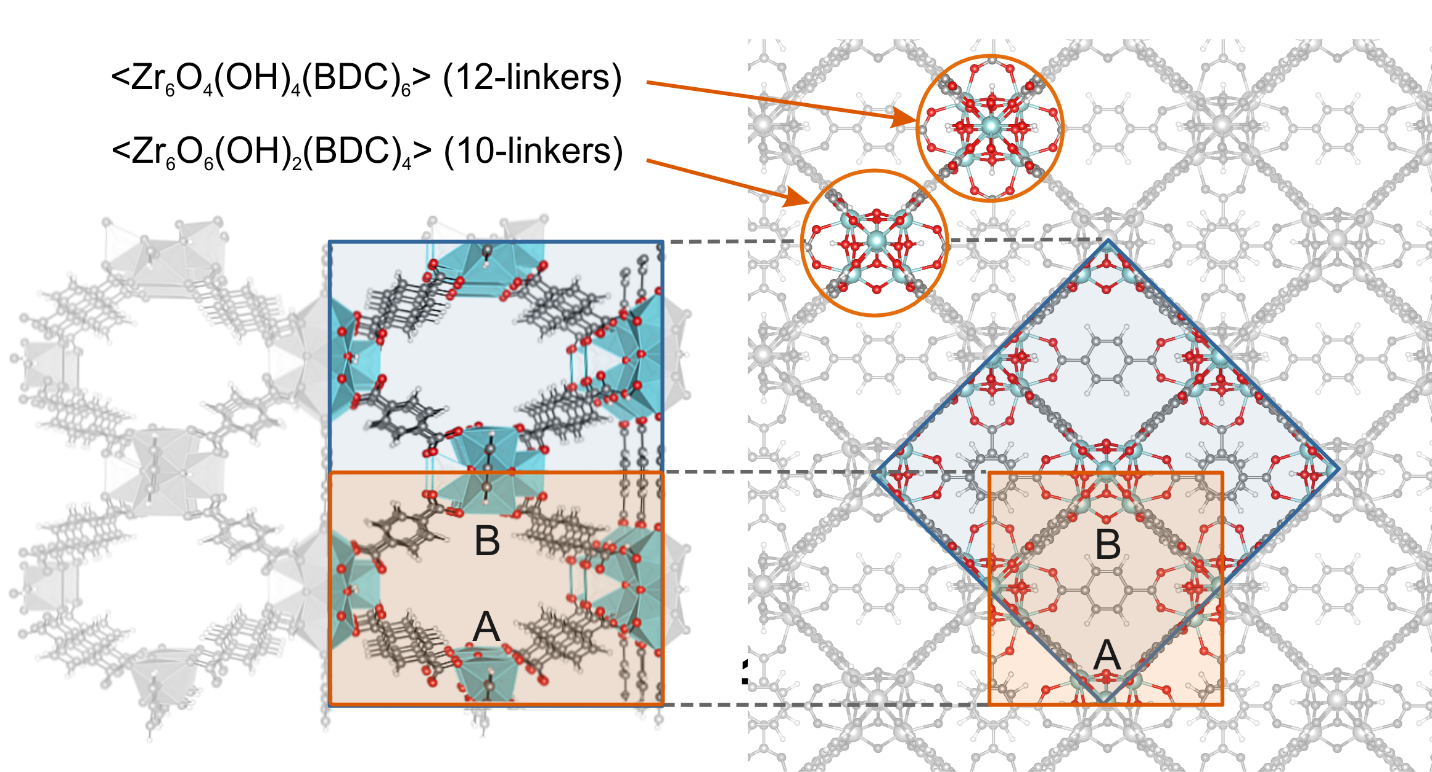
\includegraphics[width=1.0\textwidth]{periodic}
	\caption{Representation of the different ways to remove up to three linkers from a 4--brick UiO-66 unit cell}
	\label{fig:periodic}
\end{figure}

\section{Theoretical methods}
\subsection*{Electronic energy methods}
A basic quantity to study any chemical or physical transformation is the potential energy surface (PES), which is a function of the coordinates of all the atoms of the system. The PES is always the reference quantity in our simulations and every atomic configuration can be represented as a point in this hypersurface, with a given value of potential energy (Figure \ref{fig:BO-approx}).
\npar
Ideally, by calculating the value of the PES for each atomic configuration we can obtain all information on the system and on the transformations that can occur. However, the complexity of this surface escalates quickly with the number of atoms, and the sampling of its relevant regions represents the main challenge of molecular simulations. The information gained by exploring the PES is tightly connected to the experimental observables. Statistical physics acts like a bridge between the microscopic insight that is gained through molecular simulations and the macroscopic properties which are measured experimentally. In principle, all macroscopic properties of a system can be derived from its wavefunction. To calculate it, the stationary Schr\"{o}dinger equation is solved: 
\[
\hat{H}\left\vert\psi\right\rangle = E\left\vert\psi\right\rangle
\]

where $\psi$ is the wavefunction, $\hat{H}$ is the Hamiltonian of the system, and $E$ is the total energy. The resolution of this equation is at the heart of computational chemistry and will in principle provide the exact description of matter, but it is nevertheless extremely difficult to solve for most of the electron systems. The presence of electron--electron interactions makes it a highly coordinated problem, and for this reason, different approximations need to be applied, to remove the interactions that have a minimal contribution to the energy.

\subsection*{Born--Oppenheimer approximation}

\begin{figure}[!htbp]
	\centering
 	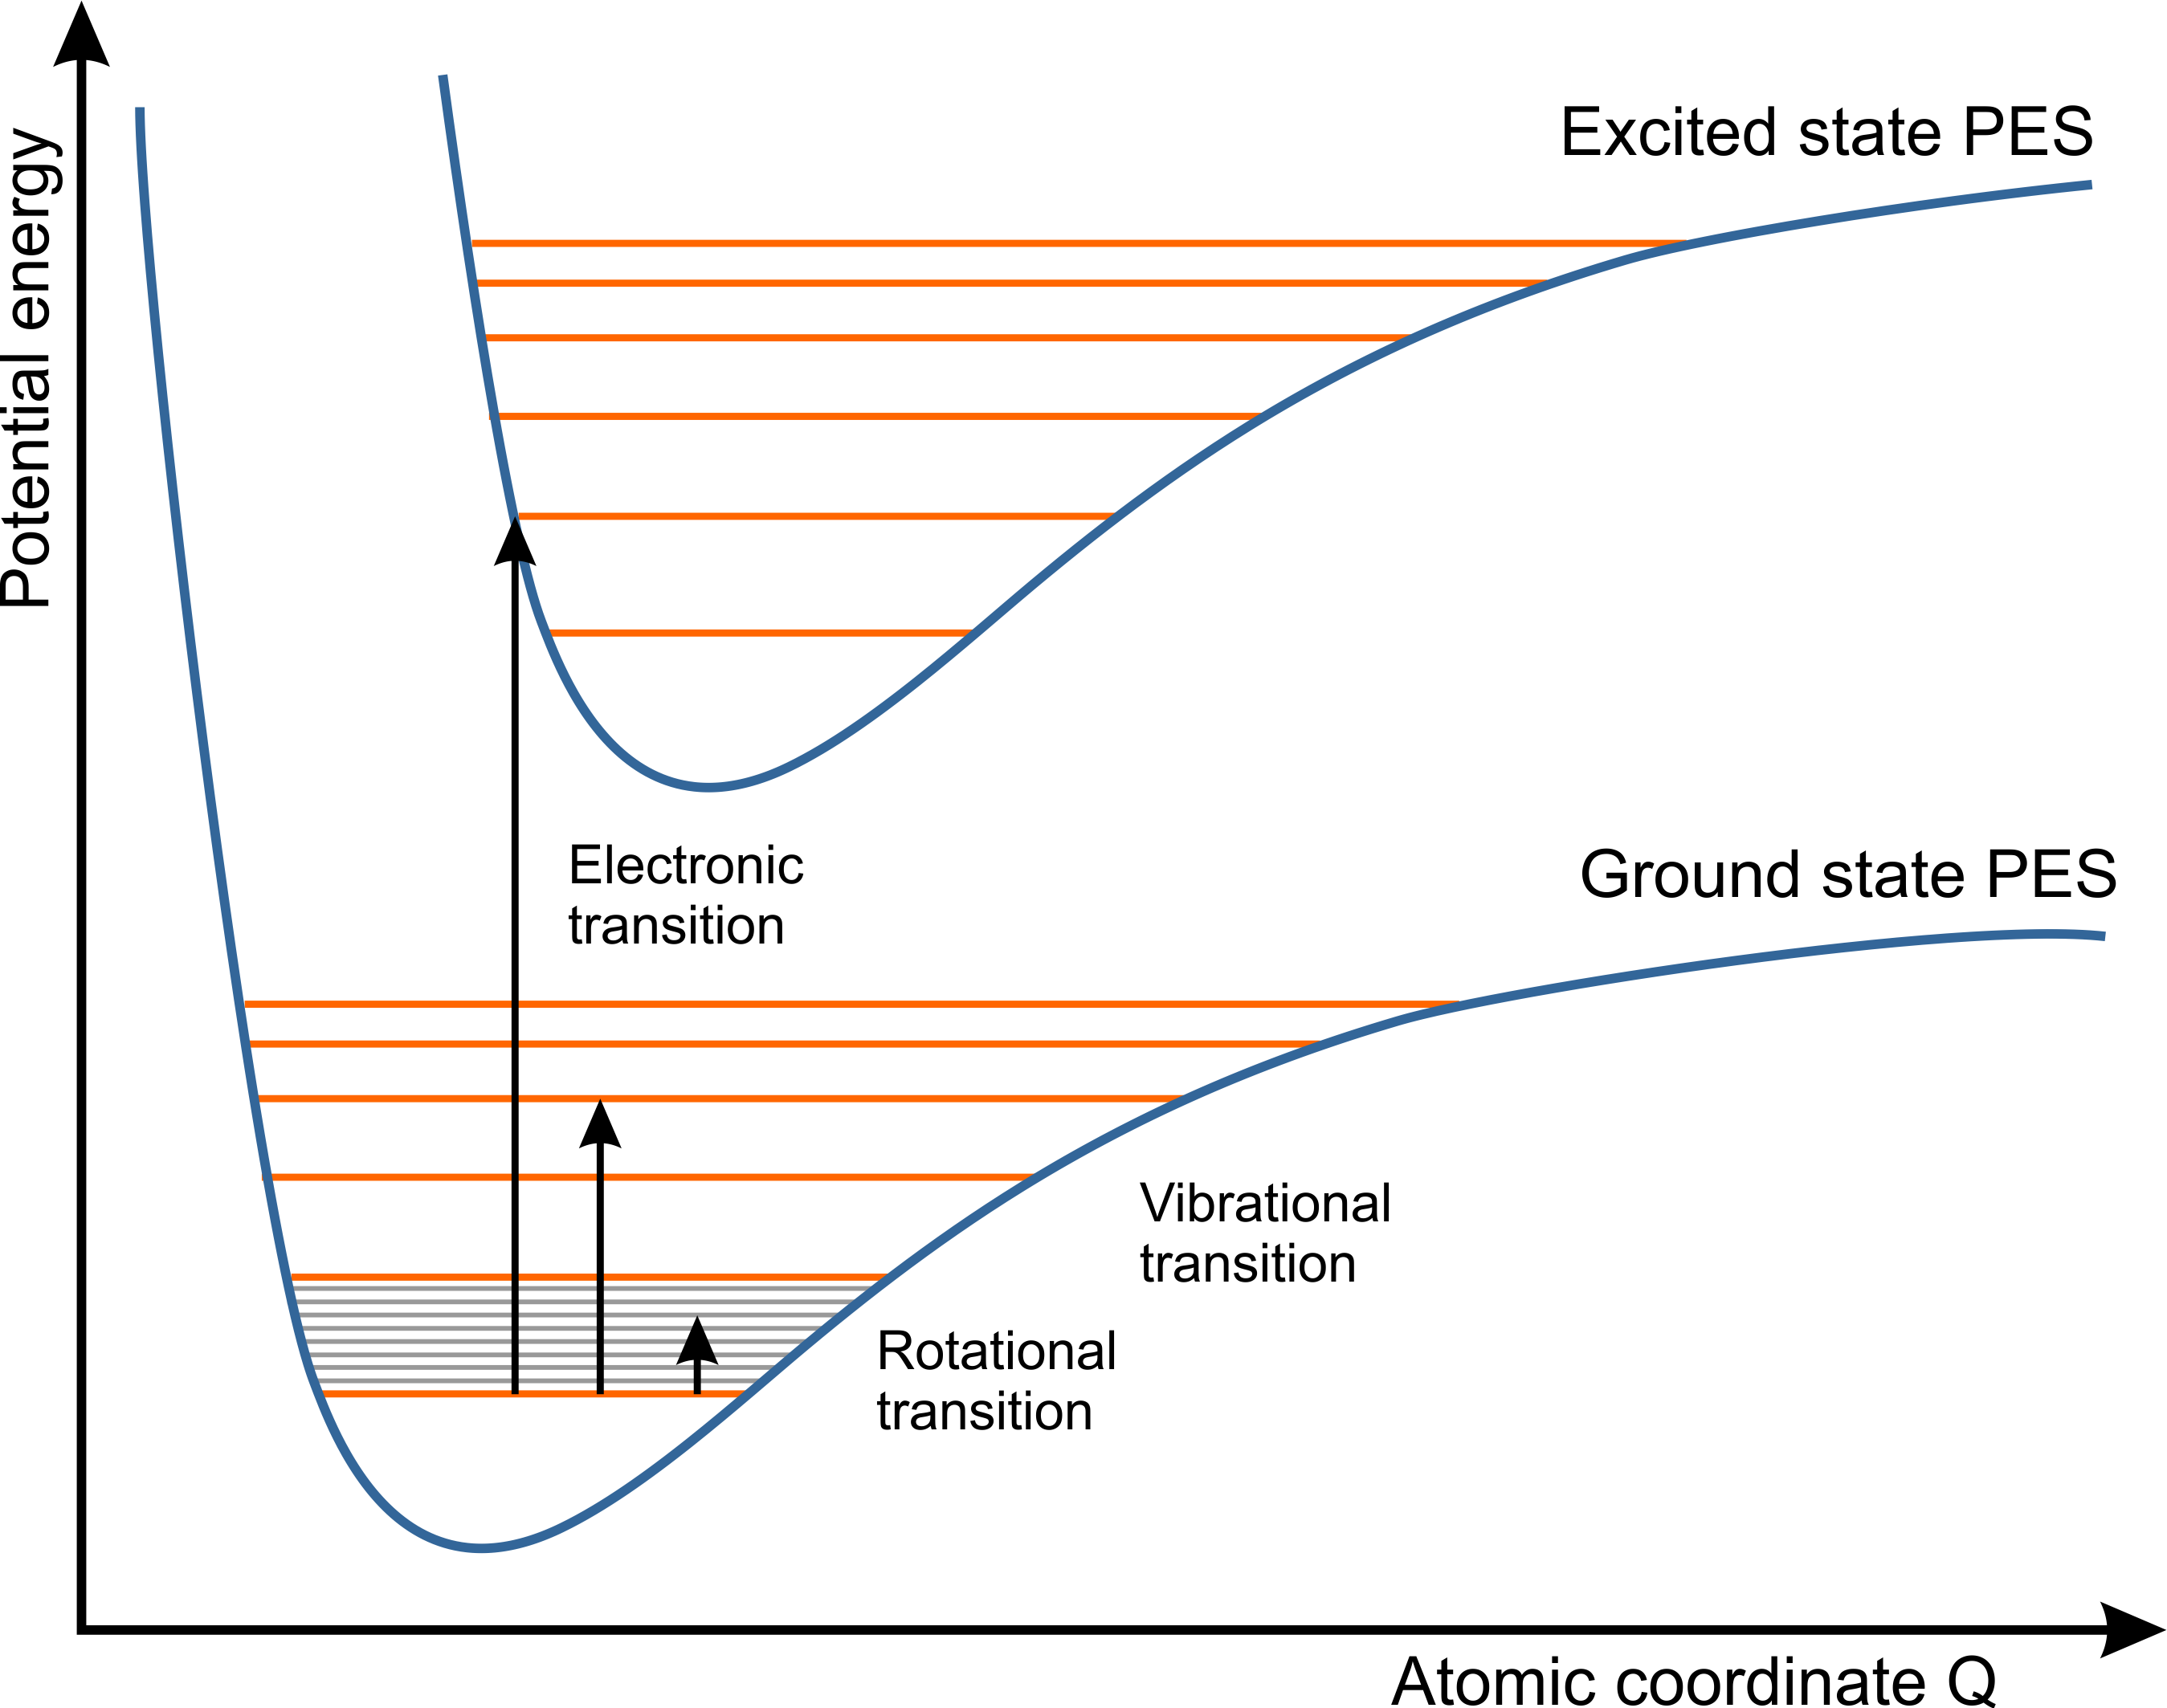
\includegraphics[width=1.0\textwidth]{BO-approx}
	\caption{The two lowest PES in the BO approximation for a diatomic molecule. In blue, the electronic PES for the ground state and first electronic excited state (UV--Vis transitions). In orange, the vibrational energy levels (IR transitions), in grey the rotational levels (microwave transitions).}
	\label{fig:BO-approx}
\end{figure}

For all calculations performed in this work, we rely on the so--called Born--Oppenheimer (BO) approximation \cite{Born1927}. In this treatment, nuclei are considered as classical points which move in the potential energy surface generated by the electrons (Figure \ref{fig:BO-approx}). This way, to each nuclear configuration a corresponding electronic energy can be assigned, and nuclear coordinates enter in the Schr\''{o}dinger equation only as parameters, allowing to construct a BO surface, or PES. This approximation holds since nuclei are much slower than electrons, therefore the motion of electrons is instantaneous from the nuclei point of view. 
This approximation does not always hold, especially when dealing with light nuclei such as hydrogen. In these cases, nuclear quantum effects can have an impact on the measured properties \cite{Ceriotti2016}. In most cases, the electronic ground state is also not interacting with the higher electronic states because of the high energy difference. In the BO approximation, the electronic energy levels are also considered fully separated and do not interact with each other. For this reason, the approximation is also called adiabatic approximation. Additional interactions have to be considered when two surfaces lie close to each other, for instance in the neighborhood of conical intersections. 

\subsection*{Force Fields}

\begin{figure}[!htbp]
	\centering
 	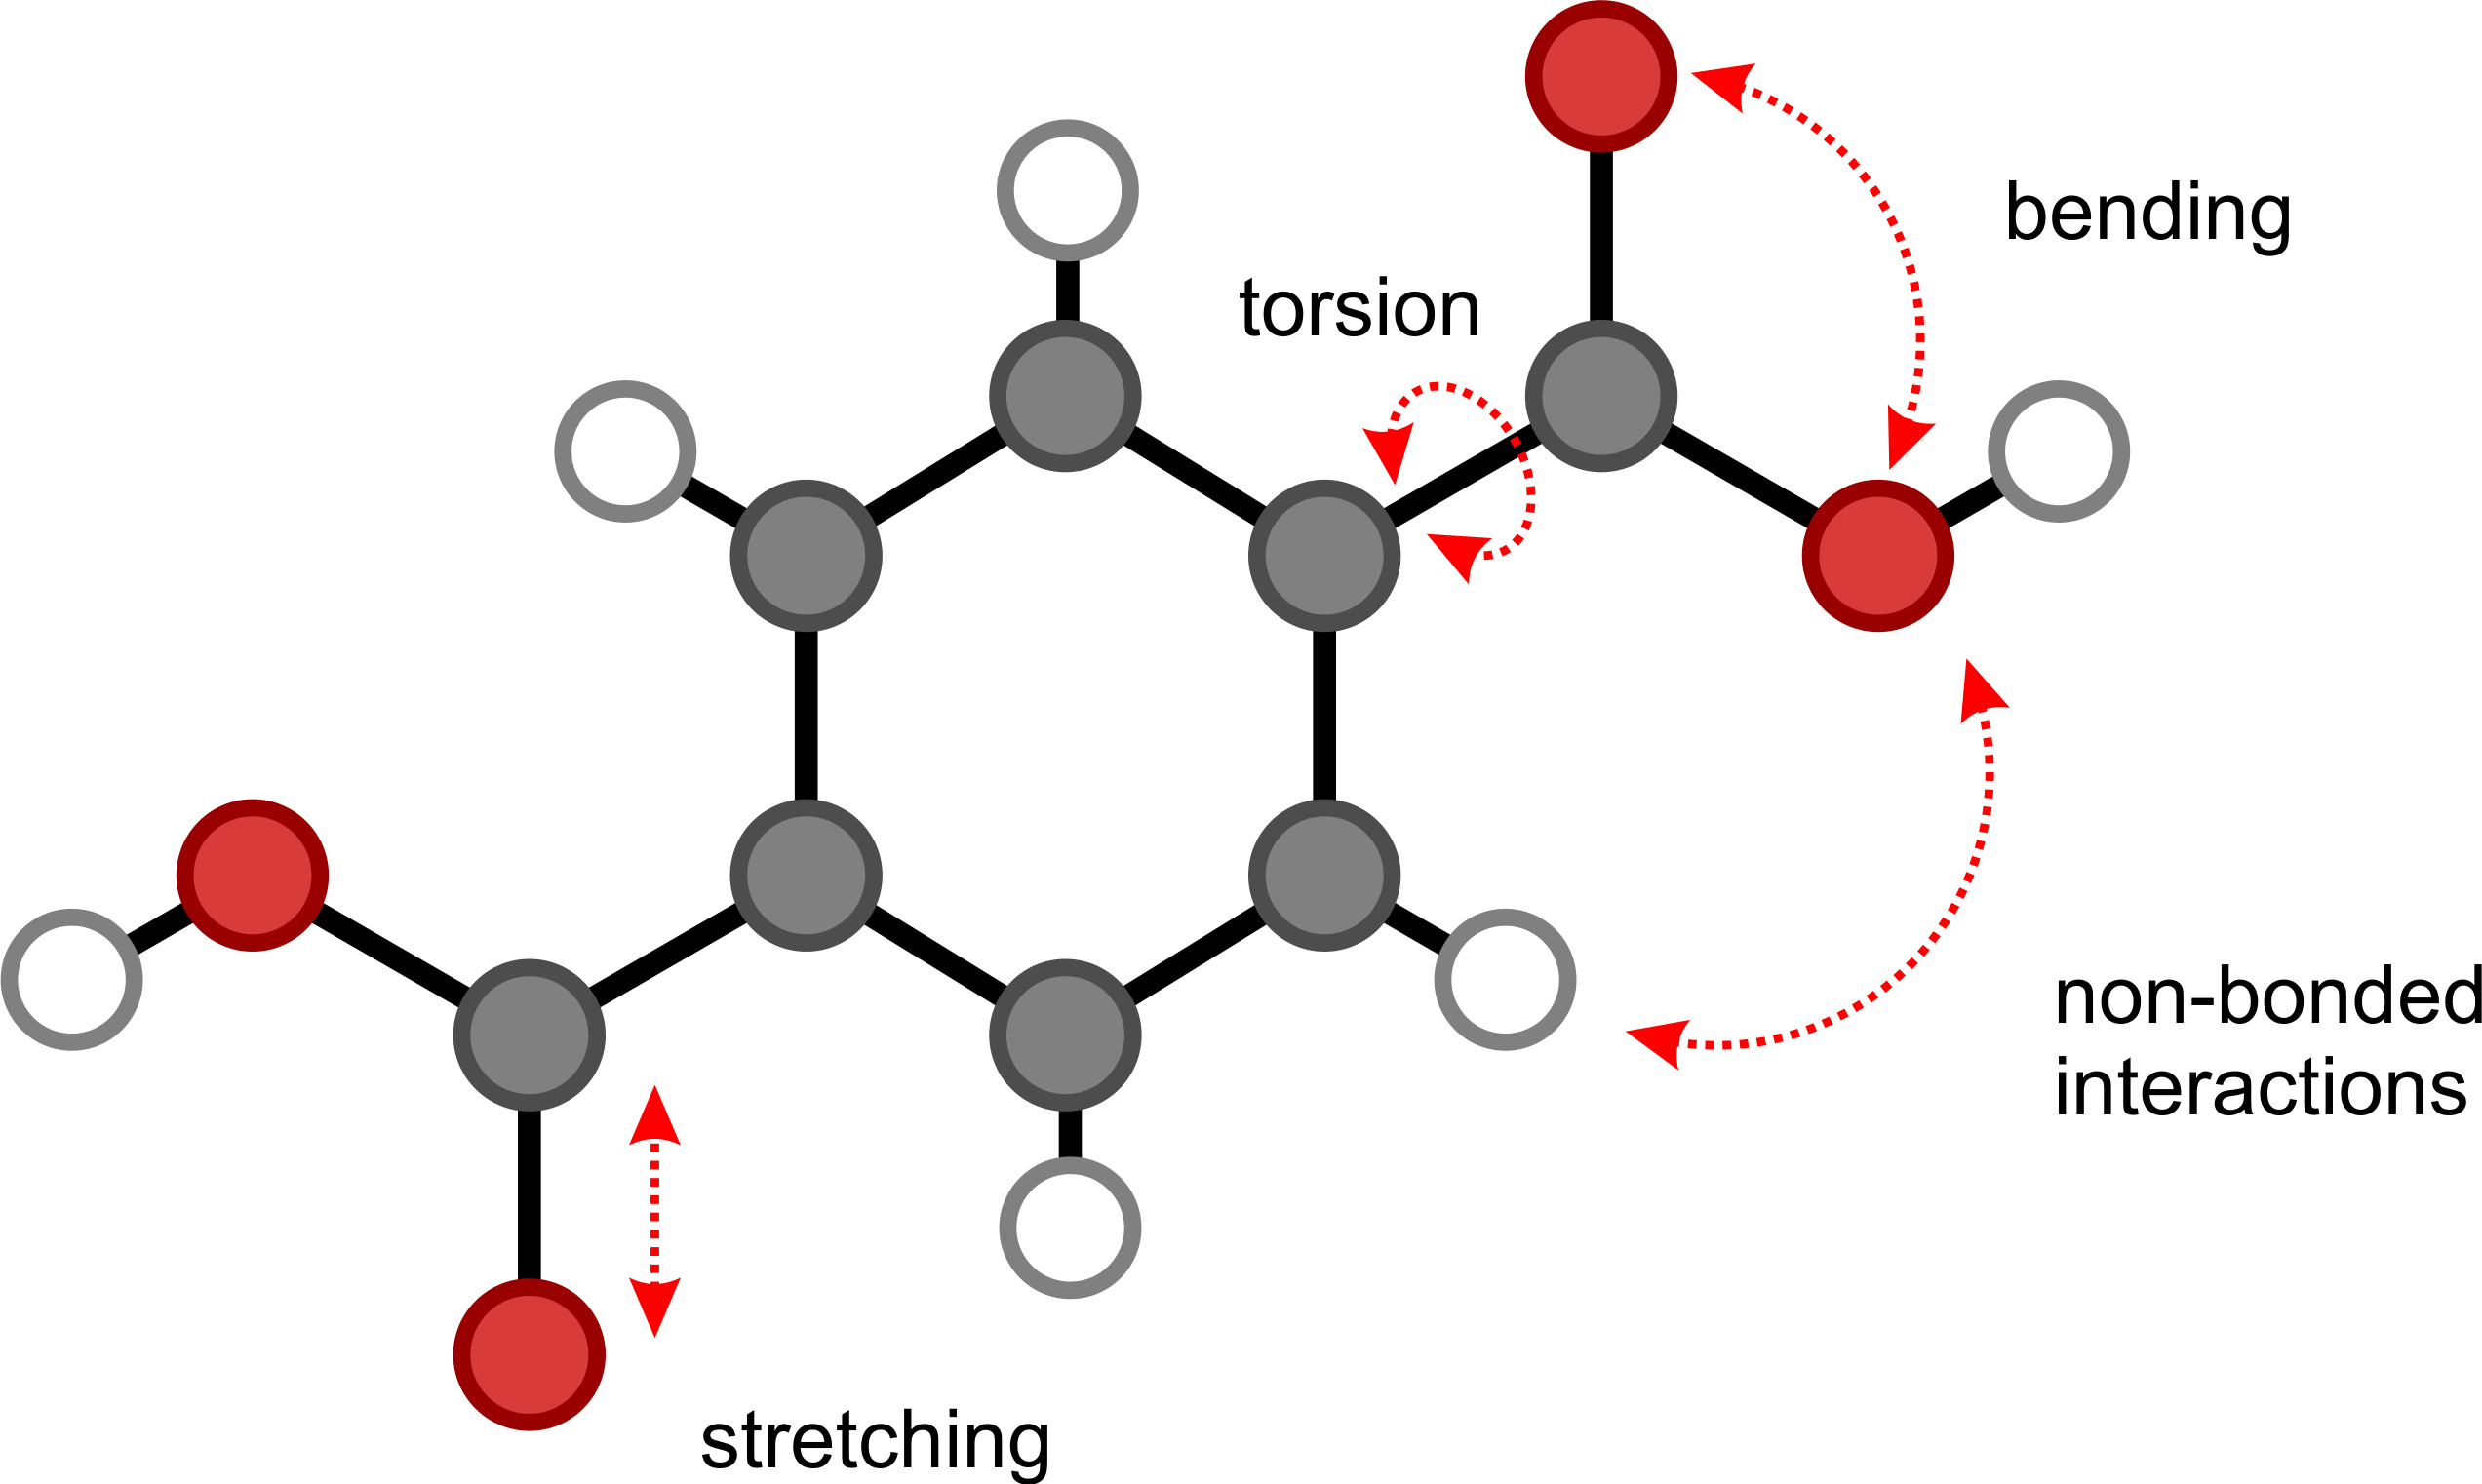
\includegraphics[width=0.7\textwidth]{forcefield}
	\caption{Representation of some of the molecular modes taken into account in a generic force field model.}
	\label{fig:forcefield}
\end{figure}

The simplest way to describe interactions between atoms which determine the PES is the so--called ``balls and springs'' model. In this treatment, all interactions are represented by interatomic classical potentials which are parametrized to reproduce the results of more accurate quantum mechanical calculations. In this work, generic force field calculations have been used in some cases to give preliminary input structures for more costly \textit{ab initio} calculations, through which the description of chemical transformations is possible. 
Force fields are often constituted by harmonic potentials which do not allow bonds being broken and formed (Figure \ref{fig:forcefield}). Reactive force fields, such as ReaxFF \cite{VanDuin2001} are currently being developed, but their application in complex heterogeneous reactions is still an ongoing chemical challenge and is out of the scope of this work. For this reason, the description of reactive processes needs a more advanced treatment, where electronic distributions are explicitly taken into account.

\subsection*{Density Functional Theory}
Density functional theory (DFT) has become the method of choice for the study of chemical systems, due to its good trade--off between computational cost and accuracy of the obtained results. DFT began in the 1920’s with the work of Thomas and Fermi \cite{Thomas1927, Fermi1928}, but it was only in the ’60s that it became a complete and accurate theory, shown in the work of Kohn, Hohenberg and Sham\cite{Hohenberg1964}. The fundamental property that DFT describes is electron density as opposed to many body electron wavefunctions, which allows to reduce enormously the number of variables in the case of complex systems. Two fundamental theorems by Hohenberg and Kohn state that there is a unique relation between electronic density and total wavefunction, therefore the ground state density allows us to determine all properties of the system. Moreover, the ground state density can be obtained from a minimization of the total energy functional with a variational method by solving the so--called Kohn--Sham equations. The global minimum value of the functional determines the exact ground state of the system. This way it is possible to obtain the total energy of the system and the forces which act on the atoms, two quantities which are needed in all the simulations performed in this work. 
\npar
In principle, DFT is an exact method, but the minimization of energy is far from trivial. Kohn and Sham \cite{Kohn1965} introduced a method which replaces the many--body problem with an auxiliary system of non--interacting particles, allowing a fast solution of the eigenvalue problem. What needs to be added in this treatment is an additional functional which describes exchange and correlation. Nowadays one of the greatest challenges in DFT consists in the search for an accurate expression for the exchange--correlation functional.
The simplest method is known as Local Density Approximation (LDA) initially proposed by Kohn and Sham \cite{Kohn1965} and can also be adapted to include spin in the Local Spin Density Approximation (LSDA) \cite{Vosko1980}. A more refined method is the Generalized Gradient Approximation (GGA) which involves the calculation of the gradient of electron density and includes functionals such as B88 \cite{Becke1988}, LYP \cite{Lee1988} and PBE \cite{Perdew1996, Perdew1997}, used in this thesis. 
 More recent functionals are the so--called hybrid functionals, which include the Hartree--Fock (HF) exchange, such as B3LYP \cite{Becke1988, Becke1993, Lee1988}, which is a combination of B88, LYP and LDA with HF, and PBE0 \cite{Adamo1999}, which mixes PBE with HF. These functionals can give a more accurate electronic description of the system but are computationally very expensive. As compromise between accuracy and computational cost is a geometry optimization with PBE, and a single point calculation to refine the energies with B3LYP, as performed in \textbf{PAPER I}.

\subsubsection*{Dispersion interactions}
In this thesis we often encounter noncovalent interactions which need to be treated with high accuracy, such as the adsorption of guest molecules on the zirconium Lewis acid sites or interaction between solvent molecules. One of the challenges of DFT methods is the description of long range dispersive interactions such as London forces, which are commonly referred to as van der Waals interactions. These interactions are due to many particle electron correlation effects which are present also in absence of charges and can have a significant impact on the noncovalent interaction energy. To tackle this problem, various dispersion schemes have been proposed. One of the most used is currently the Grimme--D3 method \cite{Grimme2010}, where a damped $-C_{6}R^{-6}$ function is added to the DFT functional. Recently, more advanced dispersion schemes have been developed, such as the many body dispersion scheme \cite{Buko2016}, or the one of Tkatchenko and collaborators \cite{Ambrosetti2014}, although for the systems we are studying not many benchmarks of these new methods have been performed so far \cite{Wieme2018}.

\subsection*{Geometry optimization}
In order to obtain molecular structures that have physical significance and their relative energies, the arrangement of the atoms needs to be optimized. There are generally two types of molecular structures that we need to find in our simulations, the equilibrium geometries, which correspond to \textit{minima} of the PES, and the transition state geometries, which correspond to first order saddle points, as displayed in Figure \ref{fig:PES}. These points are characterized by null first derivatives of the energy (the total forces acting on each atom are sufficiently close to zero), all positive second derivatives for local \textit{minima} and one negative second derivative for first order saddle points, which correspond to transition states. 

\begin{figure}[!htbp]
	\centering
 	\includegraphics[width=1.0\textwidth]{PES}
	\caption{Schematic representation of the potential energy surface and the stationary points.}
	\label{fig:PES}
\end{figure}

The geometrical optimization of reactants and products consists in a minimization of the energy along the nuclear coordinates. Often the starting point is the experimental structure which can be obtained from diffraction data. In the most used codes several minimization methods are implemented, each characterized by a different computational cost and robustness, such as steepest descent, conjugated gradient or simulated annealing. The algorithms will find local \textit{minima}, and do not guarantee that the system will be in a global \textit{minimum}, therefore the minimizations must start from a sufficiently good guess. 
\npar
The search for transition states is far from trivial and often requires an iterative procedure involving different methods and requiring a good knowledge about the system and chemical process under study. In the calculations performed in this thesis, we often start from an equilibrium structure and as a first guess, we adapt the bond lengths and angles to be close to the transition state with a molecular editor such as Zeobuilder \cite{Verstraelen2008}. These bond lengths are then fixed, and the rest of the structure is reoptimized. The Hessian of this partly optimized structure needs to be then computed, and the vibrational modes analyzed, to check which (if any) negative frequency corresponds to the transition state. The system can be optimized again without the constraint using an improved dimer method along a selected eigenvector \cite{Heyden2005} which is followed by the optimization with a \textit{quasi}--Newton method \cite{Press1989}. In some difficult cases, the TS search can be initiated on simpler cluster models and optimized in a code in which methods are usually implemented to directly find the TS structure. This way, a first guess of the TS geometry might be obtained and further transferred to the periodic model. In both transition states and \textit{minima}, if there are superfluous negative frequencies, these need to be removed. Often, it is sufficient to minimize the energy along that vibrational mode. Single point energy calculations can be performed for different values of the displacement along that mode, and the lowest point in energy can be used as starting point for a subsequent minimization of all the coordinates.

\subsubsection*{Cell optimization}
In the case of periodic systems, not only the structure, but also the unit cell needs to be optimized. This is not trivial, as when using a finite plane wave basis set the number of plane waves depends on the volume of the unit cell. If the volume changes during the optimization, artificial forces which go under the name of Pulay stress can arise. This would require many iterations to optimize the volume. In this thesis, another approach was used \cite{Vanpoucke2015} which relies on an equation of state fit. For a given volume, for instance taken from experimental data, the unit cell is optimized. Then a set of equally spaced different volumes is defined and for each of these points the geometry and unit cell parameters are optimized. This way it is possible to construct an energy--volume curve, which for a rigid system can be fitted with a Birch--Murnaghan equation of state \cite{birch1947finite,murnaghan1944compressibility}, allowing to extract the volume $V_0$ which corresponds to the \textit{minimum} electronic energy $E_{0}$. 
\[
E(V) = E_{0} + 
\dfrac{9V_{0}B_{0}}{16}
\left\lbrace 
\left[\left(\dfrac{V_{0}}{V}\right)^{\frac{2}{3}} - 1\right]^{3} B'_{0} +
\left[\left(\dfrac{V_{0}}{V}\right)^{\frac{2}{3}} - 1\right]^{2}
\left[6 - 4\left(\dfrac{V_{0}}{V}\right)^{\frac{2}{3}}\right]
\right\rbrace
\]
Where $B_0$ and $B'_{0}$ are the bulk modulus and its derivative. A new structure is then generated at this given volume and coordinates and unit cell parameters are optimized again.

\subsection*{Molecular vibrations}
As seen in the previous paragraph, for many purposes in this thesis we need to calculate the second order derivatives (Hessian matrix) of the PES, which are associated to molecular vibrations. First of all, the Hessian gives us information about the curvature of the surface and the nature of the stationary points encountered during the minimization. The second order derivatives are obtained by displacing the atoms in the three directions and calculating the energies, then the Hessian is diagonalized to determine the eigenvectors that correspond to the vibrational motions.
From the Hessian we can calculate the vibrational frequencies, which open the door to a lot more information on the system than a single point calculation. As a matter of fact, single point calculations are performed at 0 K, but even at this temperature nuclei vibrate around their equilibrium positions, and this movements are responsible for vibrational entropy. We can approximate these motions with those of harmonic oscillators, by using the vibrational frequencies constructed from the Hessian. 
\npar
\begin{figure}[!htbp]
	\centering
 	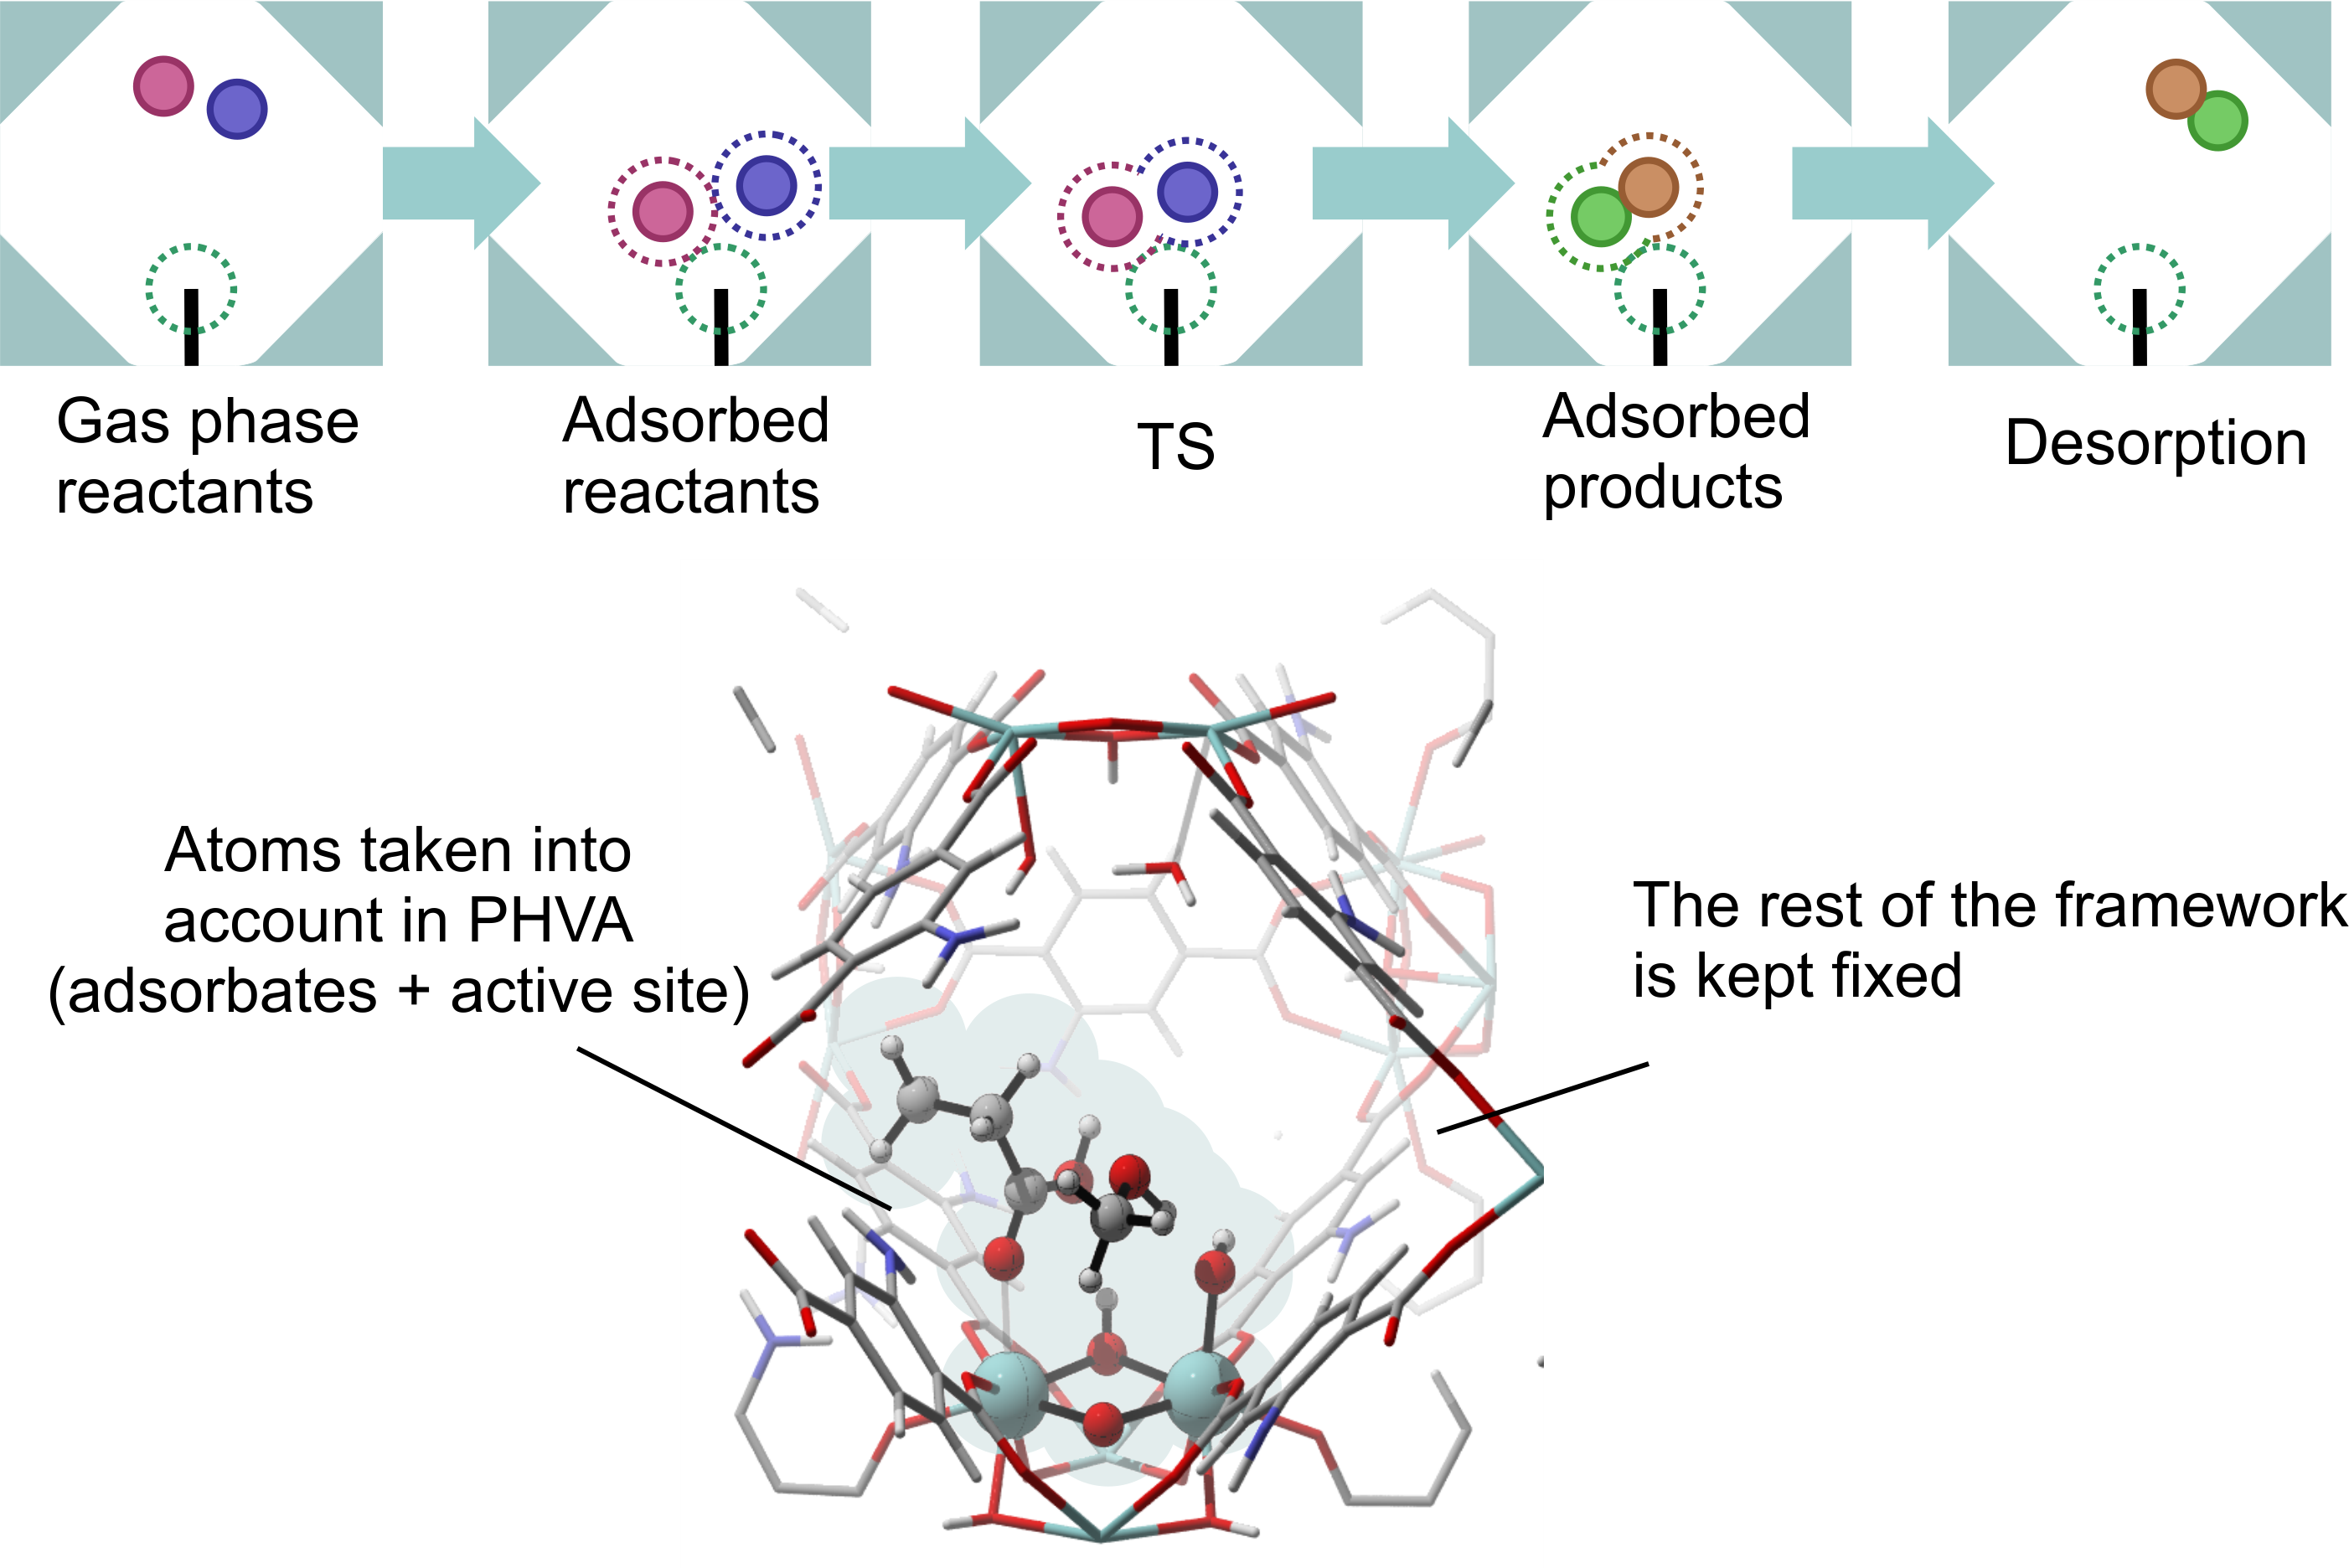
\includegraphics[width=1.0\textwidth]{PHVA}
	\caption{Representation of the atoms taken into account in the Partial Hessian Vibrational Analysis (PHVA) approach. Top: a schematic representation of a reactive process in nanoporous material, bottom: a snapshot from the static calculations where the atoms of the active site and the adsorbates are highlighted}
 \label{fig:PHVA}
\end{figure}
These frequencies can then be used to estimate the value of the vibrational entropy at finite temperatures, as will be explained later. In the calculations performed in this thesis, due to computational limits, a partial Hessian approach (PHVA) was used when dealing with reactions, as implemented in the TAMkin toolkit \cite{Ghysels2010}. The quantity that needs to be derived from these calculations is the change in free energy, which mainly depends on the parts of the system that change during the reaction, in the case of a heterogeneous catalyst the active site and the adsorbed reactants. Therefore, restricting the entropy calculations only to this part of the system is a good approximation that allows to decrease enormously the computational cost \cite{Ghysels2007}. This approach has been used in the calculation of the free energy barriers for the Fischer esterification on UiO--66 (\textbf{PAPER I}), where the atoms taken into account were the adsorbed reactants and four atoms of the active sites in their immediate proximity, as displayed in Figure \ref{fig:PHVA}.

\section{Free energy}
The central thermodynamic quantity that determines the outcome of a reaction is the free energy change associated to the process. In general, a chemical system will undergo changes in a direction that minimizes its free energy, until an equilibrium is reached. Knowing the difference in free energy between reactants and products allows us to know the equilibrium constant for a given reaction. The Gibbs Free energy can be decomposed in an enthalpic and an entropic contribution, that can be evaluated from the simulations knowing the molecular partition functions. Initially, the total internal energy $U$ has to be obtained from the electronic energy $\varepsilon_0$, the zero--point vibrational energy $E_{ZPE}$ and the molecular partition function $Q$ at constant number of particles $n$ and volume $V$:
\[
U = U_{0} + R T^{2}\left(\frac{\partial \ln Q}{\partial T}\right)_{n,V}
\]
\[ U_{0} = \varepsilon_{0} + E_{ZPE} \]
Where $R$ is the gas constant, equal to the product $N_{A}\cdot k_{B}$ between Avogadro's number and Boltzmann constant. The molecular partition function $Q$ can be split in its translational, rotational, and vibrational components:
\[
Q = Q_{trans}Q_{rot, ext}Q_{vib}
\]
The enthalpy $H$ corresponds to the total energy plus the work associated to the change in volume.
\[
H = U + p_{0}V
\] 
%H = U + p_{0}V = U + R T
The entropy $S$ can be directly obtained from the partition function:
\[
S = R \ln Q + RT \left(\frac{\partial \ln Q}{\partial
T}\right)_{n,V}
\]
Finally, the Gibbs free energy $G$ will be:
\[
G = H - TS = U_{0} + p_{0}V - RT\ln Q
\]
Where in the case of non--interacting particles $p_{0}V = RT$ following the ideal gas law. We can therefore define a free energy surface (FES) that is function of coordinates of the system, and can be derived from the PES.

\subsection*{Equilibrium}
As explained above, there is a tight connection between free energy and equilibrium concentrations in chemical reactions. As an example, an equilibrium which is of utmost importance in chemistry is the acidic dissociation of species in aqueous solution:
\[
\ce{HA + H2O <=> A- + H3O+}
\]
The acidic dissociation constant ($K_a$) is an important equilibrium constant in chemistry and is equal to the ratio between the concentration of products and reactants when the reaction reaches the equilibrium. It is often reported with its negative decimal logarithm as $pK_a$.
\[
K_a=\dfrac{\ce{[A- ][H+ ]}}{\ce{[HA]}} 
\]
The equilibrium constant is equal to the Gibbs free energy change from reactants to products.
\[
\Delta G = RT \ln K_a
\]
\[
pK_a = \dfrac{\ln 10}{RT} \Delta G
\]
Therefore, knowing the Gibbs free energy difference between reactants and products, we can have important information about the equilibrium composition of a chemical system. However, kinetic factors can sometimes play a major role, and equilibrium cannot always be easily reached.

\subsection*{Transition state theory}
A chemical reaction is a process that through rearrangement of the atoms transforms one stable state into another. Every elementary reaction can be represented as a minimum energy path connecting two \textit{minima} along the FES. Furthermore, along this reaction path the existence of a saddle can be postulated, which is the highest point in energy that needs to be crossed to go to the product state. 
The saddle point is typically called transition state or activated complex and it is the basis for the transition state theory (TST) developed by Eyring in the 1930’s, one of the most successful chemical theories which allows to explain reaction rates of elementary chemical reactions. The assumption of the theory is that there is a \textit{quasi}--equilibrium between reactants and activated complex, and the rate constant can be obtained by the size of the energy barrier and by the frequency at which the system can cross the barrier. This is possible because the barrier acts as a bottleneck in the reaction, its crossing is a rare event and all the kinetics depends only on it. For a unimolecular reaction, the rate constant can be derived from the partition functions of reactant, TS and their energy difference:
\[
k(T) = \dfrac{{k_B T}}{h}
\dfrac{{q_{TS,\ddagger}}}{{q_R}} e^{- \frac{\Delta E^{\ddagger}}{k_B T}}
\]
Where $k_B$ is the Boltzmann constant, $h$ is the Planck constant, $q_R$ and $q_{TS,\ddagger}$ are the molecular partition functions of reactants and activated complex for all coordinates except the reaction coordinate, evaluated from the zero--point vibrational level. 
\[
q_{vib,i} = \prod_{i=1}^{N_{dof}} \dfrac{1}{1 - e^{- \frac{h \nu_{i}}{k_B T}}}
\]
Where $N_{dof}$ is the number of vibrational degrees of freedom of the system. The energy difference $\Delta E^{\ddagger}$ includes electronic energy and zero--point vibrational energy difference at 0 K:
\[
\Delta E^{\ddagger} = E_{0}^{TS} - E_{0}^{R} + \Delta E_{0,vib}
\]
\[
\Delta E_{0,vib} = \sum_{i=0}^{N_{dof}-1} \frac{h \nu_{i}^{TS,\ddagger}}{2}
- \sum_{i=0}^{N_{dof}} \frac{h \nu_{i}^{R}}{2}
\]
This theory has some limitations, and may fail in the case of labile intermediates, when nuclei deviate from a classical behavior, or at high temperatures. For a given reaction, in fact, there will be many paths characterized by different barriers, and at low temperature only the lowest one will be likely to be crossed. When the kinetic energy is high enough, many other paths will be activated. The transition state will occupy a larger region of the PES, and it will not be possible to derive entropy from the vibrational partition functions.
\begin{figure}[!htbp]
	\centering
 	\includegraphics[width=1.0\textwidth]{static-scheme}
	\caption{1D free energy profiles for a given reaction with and without catalyst, indicating the adsorbed initial, final states and the localized transition state, schematically illustrated in below. The adsorption free energy, intrinsic and apparent barriers are obtained by static calculations and indicated by $\Delta G_{ads}$, $\Delta G_{\ddagger}$, and $\Delta G_{app}$, respectively;}
	\label{fig:static-scheme}
\end{figure}

\section{Exploring the free energy surface}
Static calculations, where molecular vibrations are approximated using harmonic oscillators, can fail to give an accurate representation of the entropy when there is a high configurational freedom. When the FES is flat with respect to $k_B T$, the system at equilibrium can evolve in a larger region of the PES and move along more than one \textit{minimum}. In this case, vibrational frequencies are anharmonic and it is not possible to represent the system by approximating around one single \textit{minimum} (Fig. \ref{fig:static-dynamic}). Therefore, static calculations are not always sufficient in describing the system at operating conditions. In this view, molecular dynamics (MD) techniques, which follow the time evolution of the system, can resolve this shortcoming.
\begin{figure}[!htbp]
	\centering
 	\includegraphics[width=1.0\textwidth]{static-dynamic}
	\caption{a) 1D free energy profiles for a given reaction on two different active sites in UiO--66 (insets), indicating the adsorbed initial and final states and the localized transition state for this reaction; (b) possible 2D representation of the given reaction on the two active sites as obtained using advanced dynamic techniques, indicating the three critical points on the potential energy surface.}
	\label{fig:static-dynamic}
\end{figure}

\subsection*{Ab initio Molecular Dynamics}
From MD simulations, thermodynamic properties such as free energy can be obtained taking into account a whole region of the PES instead of a single point. This is based on the ergodic theorem, that in one of its formulations states that the time average of equilibrium properties is equal to the ensemble average, in the limit of a sufficient long simulation. 
\npar
MD simulations are based on solving Newton’s equations of motion:
\[
M_i \ddot{\mathbf{R}}_i = \mathbf{F}_i = - \nabla_i V
\]
where $M_i$ and $\mathbf{R}_i$ are the mass of a given nucleus and its coordinates, $\mathbf{F}_i$ the forces that act on it, which correspond to the gradient $\nabla_i V$ of the PES. There are many ways to calculate these quantities and to integrate the equations of motion, and at present time, chemists and physicists can choose between a plethora of MD techniques which span a whole range of complexity, accuracy and computational cost. 
In the calculations performed in this thesis, potential energy and forces on the PES are calculated from first principles by means of DFT to account for the full dynamic behavior of the material by ab initio molecular dynamics (AIMD). The calculation of electronic properties which define the PES is decoupled from the propagation of nuclear motions, in a method called Born--Oppenheimer Molecular Dynamics (BOMD). Other famous AIMD methods, which differ by how the calculations of electronic potential and the equation of motion are combined, are the Car--Parrinello MD (CPMD)\cite{Car1985}, where a fictitious electronic kinetic energy is added to the lagrangian, or the Ehrenfest MD, based on the namesake theorem \cite{Ehrenfest1927, Marx2009}. 
\npar
The first MD calculations were performed in the microcanonical (NVE) ensemble, where total energy, number of particles and volume are fixed. However, in experiments it is often the temperature that is fixed, not the energy. In general, the choice of the ensemble depends on the thermodynamic quantities that need to be determined. Nowadays there are many thermodynamic ensembles in which the simulation can be performed. The most convenient for a comparison with experiments are the canonical (NVT), with fixed number of molecules, volume and temperature, or the isothermal--isobaric (NpT), with fixed number of molecules and temperature, but where the volume can fluctuate. In order to have a fixed average temperature, some control of the kinetic energy of the atoms is needed. Various thermostats, which differ in terms of speed and robustness, are implemented in every MD code. In this thesis, Nose’--Hoover thermostat was used, where the system is connected to a heat bath. The pressure is also controlled in simulations by means of a barostat. The most commonly used is the one developed by Martyna, Tobias, and Klein (MTK)\cite{Martyna1994}.

\subsubsection*{Radial distribution functions}
From MD trajectories, different macroscopic properties can be derived. An important structural property is the radial distribution function (RDF) or pair correlation function $g(r)$, that describes the probability density between specific atoms as a function of the distance, normalized with respect to a probability distribution of a homogeneous gas with the same density. The RDF can be calculated from the following expression:
\[
g_{ij}(r) = \dfrac{dn_{ij}(r)}{4\pi r^2 dr \rho_i}
\]
where $dn_{ij}/dr$ represent the number of atoms of type $j$ within a certain distance of the atoms of type $i$, and $\rho_i = V / N_i $ represent the density of the homogeneous distribution. The integral of the RDF can also give valuable insight into the number of atom pairs at a given distance, such as what is the average coordination of a certain chemical species.

\subsubsection*{Vibrational density of states}
Information on the time evolution of certain quantities in the system can be obtained by calculating time autocorrelation functions. The correlation of a certain variable with itself is equal to:
\[
\left\langle X(0):X(t)\right\rangle = \lim_{N \to \infty} \dfrac{1}{T}\int_{0}^{T}X(t)X(t+\tau)d\tau
\]
Autocorrelation functions offer a measure of the response of the system to a given stimulus, which is function of the density of states. The response of a system to a perturbation is equal to the power spectrum of the autocorrelation function of the fluctuations of the involved observable\cite{kubo1957statistical}. For instance, by calculating the power spectrum of the atomic velocities autocorrelation function, we can obtain the vibrational density of states, as done in \textbf{PAPER IV}. These spectra contain all the dynamic and anharmonic information that is neglected in the static frequency calculations.

\subsubsection*{Towards modeling at operating conditions}
With the growth in computational time, the new challenge is constituted by modeling the system at operating conditions. Many chemical reactions, especially when performed at mild conditions, involve the presence of a solvent. In order to move closer to modeling the system at operating conditions, the solvent in the pores can also be taken into account. This adds a lot of degrees of freedom to the system, and for this reason often an implicit description of the solvent is done, such as in the Polarizable Continuum Model (PCM)\cite{cances1997new}. In the case of the work in this thesis, however, it is necessary to fully model the solvent molecules, as they are actively involved in proton transfers. To do so, the number of solvent molecules that can fit in the unit cell needs to be estimated. Monte Carlo method (MC) is an alternative approach to MD to explore the PES for complex systems. It was initially developed for the calculation of multidimensional integrals and is nowadays largely used in chemistry, especially when dealing with adsorption. In the framework of this thesis, it has been applied in the Grand Canonical ensemble ($\mu VT$, fixed chemical potential, volume and temperature) to determine the number of solvent molecules that could fill the pores of the material at standard conditions.

\subsection*{Enhanced sampling MD methods}
MD simulations can offer valuable insights into the behavior of a chemical system at equilibrium conditions. From these simulations, many properties can be extracted, such as equilibrium geometries, vibrational spectra, diffusion coefficients, structural parameters etc. Configurations associated to higher (or lower) values of potential energy will be sampled for shorter (or longer) times, and in principle, if a certain process is sufficiently sampled, based on the ergodic theorem we can know its equilibrium constant, and in turn the free energy barrier associated to it. However, chemical reactions, where bonds are broken and formed, are generally rare events that will not be sampled with a regular exploration of the PES. If the free energy barrier is high compared to $k_{B}T$, the probability that such event would spontaneously occur during the simulation time is practically none. This is especially true for complex molecular systems, in which processes occur in different time scales and that can only be simulated for a limited amount of time. For this reason, different enhanced sampling techniques have been developed to enhance the sampling of low probability regions of the free energy landscape \cite{valsson2016enhancing, laio2002escaping, sutto2012new, carter1989constrained, darve2001calculating, jarzynski1997nonequilibrium, rosso2002use, gullingsrud1999reconstructing}. Recently, enhanced sampling techniques have been successfully applied in heterogeneous catalysis to study processes at operating conditions \cite{dewispelaere2016insight, dewispelaere2015complex, vanspeybroeck2014first, cnudde2017effect, haigis2015hydrothermal, buvcko2011monomolecular, fraux2017recent}.
\npar
\begin{figure}[!htbp]
	\centering
 	\includegraphics[width=1.0\textwidth]{dynamic-scheme}
	\caption{Schematic representation of different MD techniques that can be used to explore the PES.}
	\label{fig:dynamic-scheme}
\end{figure}

There are two main classes of methods that can be used to explore rare events on the free energy surface. The first class is characterized by methods that encompass all degrees of freedom and do not need any prior information on the free energy landscape between two points. Examples of these methods are Transition Path Sampling (TPS) \cite{dellago2002transition} and Replica exchange (RE) \cite{sugita1999replica}. The other class of techniques encompasses methods in which the sampling is enhanced along certain coordinates of the system, such as Umbrella Sampling (US) \cite{torrie1977nonphysical, patey1975monte} and Metadynamics (MTD) \cite{laio2002escaping}, shown in Fig. \ref{fig:dynamic-scheme}.


\subsubsection*{Choice of collective variable}
The PES is a highly dimensional surface, defined by the positions of all atoms in the system. However, often a reactive process can be described by few important coordinates called ``collective variables'' (CVs), which are projections of the high dimensional space. In fact, what can be considered a chemical configuration is an ensemble of microstates that are different in terms of absolute coordinates of each atom, but all contribute to the same macrostate. In some cases, a simple CV can represent the reaction coordinate for the process, but often the choice is not trivial \cite{rohrdanz2013discovering}. In general, choosing the right collective variable is crucial to describe the correct process. Often geometric parameters are used, such as distances, angles, dihedrals, or combinations of the latter. When studying certain processes, a switch function such as a coordination number (CN) derived from distance information is often the preferred choice. CNs represent a smart choice compared to distances, because for each pair of atoms, the coordination is zero for distances higher than a certain threshold.
\[
\mathrm{CN} =\sum_{i,j}\frac{1-(r_{ij}/r_0 )^{nn}}{1-(r_{ij}/r_0 )^{nd}}
\] 
Where CN is defined between two sets of atoms ${i}$ and ${j}$, $r_{ij}$ corresponds to the distance between atoms $i$ and $j$, and $r_0$ is a threshold distance. The exponential parameters $nn$ and $nd$ define how sharply the function behaves around the value $r_0$. In processes such as in the ones of \textbf{PAPER V}, we considered the coordination between a zirconium atom and the oxygen atoms of the solvent water. Such collective variable allows to consider the possibility that different water molecules could decoordinate and recoordinate, defining the same macrostate for a given value of the CN. We show that such processes cannot be studied by employing distances as CVs.

\subsubsection*{Metadynamics}
Metadynamics (MTD) is a popular enhanced sampling method, used to overcome barriers in the free energy landscape, which was first proposed by Laio and Parrinello \cite{laio2002escaping, barducci2011metadynamics}. During MTD, a history dependent bias potential is added in the form of gaussian hills to the PES along a certain CV. This way, potential energy is added to already visited states, allowing to escape local \textit{minima} and explore different regions of the PES. When all states are sampled with equal probability, the free energy profile along the biased CV can be obtained from the added bias potential. As the bias is added, the system is able to evolve along all the other degrees of freedom. For this reason, this method can also provide insight into the mechanisms that occur during the exploration of the different regions of the CV, as has been done in \textbf{PAPER V}. 

\subsubsection*{Umbrella sampling}
In the umbrella sampling method, a series of biased MD simulations are performed along the chosen CV. In each simulation, a bias potential is added to constrain the system to adopt a specific value of the CV, while it can evolve along all the other degrees of freedom. This way, the whole range of the CV can be explored. As each simulation is independent, this method is highly parallelizable. The free energy profile can then estimated by using different methods to combine the information obtained from the set of simulations, such as the weighted histogram analysis (WHAM) or the multistate Bennett acceptance ratio\cite{kumar1992weighted, torrie1977nonphysical}. Even if the CV is constrained in each simulation, this method can also offer valuable insight into the evolution of the system at different values of the CV, as has been done in \textbf{PAPER III}.
\npar
\npar
\npar
\npar
\npar
In summary, this chapter gives an overview of the many methods that have been employed to understand the properties of MOFs. Reactive processes can be studied by using a plethora of different computational techniques that differ in cost and accuracy. Cluster calculations were used for a first estimate of the energies, whereas periodic models were used for all the remaining part of this thesis. The increase in computational time allowed to include more complexity in the model, and to explicitly take into account the role of solvent and structural modifications in the material. During the time frame of this thesis, we moved from a static description of the chemical events towards modeling at operating conditions that allows to better describe and predict real processes. 
\clearpage{\pagestyle{empty}\cleardoublepage}
\graphicspath{{figures/chapter3/}}
% Header
\renewcommand\evenpagerightmark{{\scshape\small Major research results}}
\renewcommand\oddpageleftmark{{\scshape\small Chapter 3}}

%\renewcommand{\bibname}{References}
\hyphenation{}
\chapter[Major research results]%
{Major research results}
\label{ch3}
This Chapter illustrates the main research results obtained in the framework of this thesis. The main goal of this work was the study of the nature of active sites on UiO--66 and MOF--808 upon activation processes, and how the solvent and the functionalization influenced their behavior. The role of active sites on defective UiO--66 was studied for Fischer esterification of free fatty acids (FFA), at it became clear that solvent played an unexpected active and beneficial role in the reaction mechanism. Different molecular modeling techniques based on static and dynamic methods have been applied to gain insight into the interaction between active sites and reactants in the material, as has been introduced in Chapter 2. Contrary to reactions in zeolites, processes in MOFs are often performed ad mild conditions in the presence of a solvent, which adds complexity to the model. So far, solvent in MOFs had been studied only with classic approaches, but with the increase in computational power it was possible to include a full \textit{ab initio} treatment of water and methanol solvent in the UiO--66 pores and to go towards an \textit{operando} description of activation processes in MOFs. The most important scientific results will be highlighted in this Chapter. More details are to be found in the original articles, enclosed in Part II.

\section{Activation processes in zirconium--MOFs}
One of the main challenges in MOF research is the understanding of how active sites are created and how they impact the properties of the material. For this purpose, molecular modeling offers a platform that allows to study such activation processes and nature of active sites at the molecular level. In this sense, UiO--66, characterized by an exceptional stability, is the perfect MOF archetype where different activation and PSM processes can take place without disrupting the stability of the structure. This MOF represents a showcase example, as the findings can in principle be extended to other MOFs that are more difficult to study.
%%
\begin{figure}[!htbp]
%\vspace{-2cm}
	\centering
	\includegraphics[width=1.0\textwidth]{UiO-66-activation}
	\caption{Schematic representation of the UiO-66 structure with possible configurations of the bricks that give rise to coordinatively unsaturated Zr atoms. The colors indicate the coordination of the Zr atoms.}
	\label{fig:UiO-66-activation}
\end{figure}
%%
\subsection{Missing linker defects}
In \textbf{PAPER I} we investigated the local defect topology upon removal of a linker on UiO--66 as starting point to investigate the catalytic role of defect coordinating species in the mechanism of Fischer esterification. When studying the catalytic behaviour of UiO--66, an essential ingredient to understand the reactivity of the inorganic SBU is the knowledge of the molecular structure of the active sites upon removal of a linker. On these sites, defect coordinating species can be adsorbed and have an impact on the catalytic properties of the MOF by introducing additional sites that can play an active role in reactions. 
%%%%%%
\begin{figure}[!htbp]
%\vspace{-2cm}
	\centering
	\includegraphics[width=1.0\textwidth]{adsorption-water}
	\caption{Coordination free energies at reaction temperature of 351 K of one, two and three water molecules at coordinatively unsaturated Zr-bricks in defective UiO--66 with respect to a water coordination free site (site R). The structure of the opposite site B corresponds with configuration 2’ with two water molecules and consistently used in all periodic calculations considered in the figure. Free energies (in black) are given in kJ/mol, and their decomposition into enthalpic $\Delta$H (blue) and entropic -T$\Delta$S (grey) contributions. Energies are resulting from periodic calculations with PBE-D3 level of theory. In each configuration Lewis acid and Brønsted sites are indicated.}
	\label{fig:adsorption-water}
\end{figure}
%%%%%%
Upon removal of one of the twelve negatively charged BDC linkers from the inorganic \ce{Zr6O4(OH)4} SBU, the positive charge left on the brick has to be compensated. Charge neutralization can be accomplished by either coordinating a negative ion such as hydroxyl group to one of the zirconium atoms, or by removing a proton from the brick. This latter case is characterized by two zirconium open metal sites, and is the type of active site that is obtained upon thermal treatment of the brick at T $>$ 423 K. It was previously accepted that these Lewis sites were responsible for the catalytic activity of UiO--66, but recent studies point towards the active role of Br\o{}nsted sites in the neighborhood of defective zirconium atoms \cite{canivet2014water, oien2014detailed, canivet2016origin, ling2016dynamic, liu2016probing, klet2016evaluation, vandichel2016water, ghosh2014water}. The presence of multiple sites makes it difficult to establish a simple structure--activity relation. In particular, it is important to understand from a mechanistic point of view how the presence of defect coordinating species may affect the catalytic activity on Zr--MOFs. This research was done in collaboration with the group of Dr. Francesc X. Llabr\'es i Xamena as experimental partners. 
\npar
The coordination of water species near the active sites can occur with different configuration schematically displayed in Fig. \ref{fig:adsorption-water}. In all structures the presence of possible Lewis and Br\o{}nsted sites which may play a role in reactions is highlighted. The simplest case taken as reference configuration is the unsaturated site obtained upon thermal activation, containing two $\mu_3$ oxygens bridging the zirconium atoms which may act as Br\o{}nsted sites. From this structure, the coordination of one physisorbed water molecule to one of the zirconium atoms is energetically favorable. A decrease in energy is observed when the molecule is deprotonated to the oxo atom as in configuration 1’. The chemisorption of this water molecule shields the Lewis character of the zirconium atom, but introduces an additional Br\o{}nsted site in proximity to the open metal site. 
\npar
The most stable configurations are observed in presence of 2 or 3 adsorbed water molecules on the adjacent zirconium atoms. Two physisorbed water molecules of configuration 2’ can be adsorbed to the two zirconium atoms, followed by an immediate dissociation of one of the two molecules into a hydroxyl group and a proton on the adjacent $\mu_3$ oxygen. This configuration is characterized by a free energy difference of -94.4 kJ/mol at reaction temperature of 351 K compared to the dehydrated defective site. The presence of two zirconium coordinating species has been reported by Lillerud \cite{oien2014detailed} by means of Single--crystal X-Ray diffraction (SXRD), showing that the material is most stable when all zirconium atoms are fully coordinated. When starting from the thermally activated material that contains open Lewis sites, at standard condition, water present in the atmosphere will immediately coordinate to restore the 8--fold coordination of the zirconium atoms to give structure 2. This structure is consistent with the one proposed by the group of Farha \cite{klet2016evaluation} who identified three types of protons from potentiometric titration: $\mu_3$--OH, \ce{Zr-OH} and \ce{Zr-OH2}. 
\npar
A third bridging hydroxyl species as charge neutralizing species was proposed by Yaghi \cite{trickett2015definitive} from XRD data. They propose two physisorbed water molecules bridged by an \ce{OH-} counterion that is stabilized by a hydrogen--bond interaction with the neighboring $\mu_3$--OH of the brick. However, a recent study Ling and Slater \cite{ling2016dynamic} did not succeed in finding a corresponding minimum on the PES. In this work, we observe that the $\mu_3$--OH atom immediately deprotonates in proximity of such \ce{OH-} anion (configuration 3). Similarly as in the previous case, this structure can further stabilized by a deprotonation of one of the two physisorbed water molecules, to yield configuration 3’ of Fig. \ref{fig:adsorption-water}, in agreement with a previous report by Vandichel et al. \cite{vandichel2016water}. Adsorption of reactants involved on the Fischer esterification reaction was also taken into account. Similar considerations on the deprotonation processes can be drawn when considering methanol instead of water as reported more in detail in \textbf{PAPER I} and \textbf{PAPER II}. The energies obtained clearly demonstrate that water molecules preferentially adsorb on the zirconium atoms and the only limit to the adsorption of more water molecules lies in the entropic penalty. 

\subsection{Nature of active sites for Fischer esterification}
 Among the reactions that can be catalyzed by UiO--66, Fischer esterification is an important process in the production of biodiesel, a biofuel that is obtained from renewable sources, such as oils and animal fats. UiO--66 has been shown to be a stable and reusable Lewis catalyst with high conversion rate for the reaction \cite{cirujano2015conversion, cirujano2015zirconium}. Experimental findings performed on both hydrated and dehydrated UiO--66 show that water has a beneficial role in the process, but a theoretical rationalization of the underlying causes was missing. Moreover, amino functionalization was shown to increase the reaction rate. To address these questions, the role of active sites on UiO--66 during the Fischer esterification reaction was studied in \textbf{PAPER I}. Two possible lowest activated reaction pathways were identified for the hydrated and dehydrated active site.
\begin{figure}[!htbp]
%\vspace{-2cm}
	\centering
	\includegraphics[width=1.0\textwidth]{esterification}
	\caption{Mechanism and free energy profile for the esterification of propionic acid with methanol on a hydrated and defective UiO-66 material (blue), a hydrated defective UiO-66 material with amino functionalization of the BDC linkers (red), and on a dehydrated defective UiO-66 (black). Periodic calculations at B3LYP-D3//PBE-D3 level of theory, T=351 K. R corresponds with an empty frame with one linker defect and a pool with all reactants to guarantee mass balance. In P the defective Zr-brick is coordinated with two water molecules (configuration 2’). P’ corresponds to the empty frame with the ester as final product and remaining water molecules in gas phase.}
	\label{fig:esterification}
\end{figure}
\npar
The proposed reaction mechanism is shown in Fig. \ref{fig:esterification}. From the reactant configuration, the physisorbed water molecule is displaced by the carboxylic acid that coordinates on the zirconium atom. The resulting configuration was identified after a series of static calculations probing possible geometries. In this configuration, the acid carbonyl group is bonded to the zirconium, and at the same time methanol is hydrogen bonded to the hydroxyl group coordinated to zirconium. The adsorption of the acid on the Lewis acid site gives to the carboxylic carbon a more electrophilic character, making it more prone to interact with the alcohol. The oxygen of methanol is at the same time made more nucleophilic due to the hydrogen--bonding interaction with the Br\o{}nsted basic site situated in close proximity. This favors the condensation between activated carboxylic carbon of the acid and methanol. Two TS are involved in the process, in which first a tetrahedric intermediate is formed, and then water is removed. In both, the hydroxyl group plays a role, first as proton acceptor, then as proton donor, while the acid maintains the bond with the carbonyl oxygen. The low energy barriers associated to the two TS are 28.9 and 30.6 kJ/mol at 351 K. The reaction can proceed both ways, until an equilibrium is reached. This mechanism is characterized by a dual participation of Br\o{}nsted and Lewis sites, and overlays with the experimental findings.
\npar
Upon thermal treatment at 423 K, UiO--66 loses the adsorbed solvent molecules without compromising the structure of the inorganic SBU, contrary to the dehydroxylation with release of two water molecule that takes part at T $>$ 523 K \cite{valenzano2011disclosing}. In principle, these open metal sites should be more catalytically active, but a decrease in catalytic activity is experimentally observed. In the proposed mechanism, two Lewis acid sites, the zirconium atoms, and one Br\o{}nsted basic site, the $\mu_3$ oxygen, play an active role in the reaction. This mechanism is characterized by three TS, in which: 1) methanol is deprotonated to the oxo atom, 2) an adduct is formed between the electrophilic carbon and the oxygen of methanol 3) the $\mu_3$--OH group deprotonates to form water. This reaction is characterized by higher activation barriers (a total barrier of 90 kJ/mol at 351 K), which explain the lower catalytic activity of the dehydrated material.
\npar
Other mechanisms that do not make use of either Lewis or Br\o{}nsted sites were investigated without success, as the energy barriers were too high to be likely to occur. Both proposed mechanisms are characterized by a dual participation of Lewis and Br\o{}nsted sites that work complementary to each other. The presence of acid and basic centers within molecular distances has been shown to be essential in the performance of the catalytic reaction as they cooperate in a concerted way during the chemical transformation. Most of the previous mechanistic studies on the UiO--66 material merely focused on the Lewis acidity of the undercoordinated sites, but it has become more an more clear that the bifunctional nature of the UiO--66 catalyst will play an important role in its future applications.

\subsection{Role of defect topology}
The adsorption of species present in the reaction environment of PSLE process was studied in the framework of \textbf{PAPER IV}. In this process, we wanted to see how defect--free and defective UiO--66 material would interact with water and methanol species. To obtain this information, we made use of a larger unit cell, to be able to represent different amount of missing linker defects. This increase in complexity reflects in the higher computational cost of modeling such structure. The defective structures taken into account in the modeling are obtained by removal of linkers from the conventional unit cell containing four inorganic \ce{Zr6(O)4(OH)4} bricks \cite{cavka2008new}. Different numbers of missing linkers were modeled, to represent the different amount of defects in the experimental samples. A case with a low amount of defects is modeled by a unit cell with one missing linker. In this structure, two bricks are 12--fold coordinated, and two bricks are 11--fold coordinated, with an average of 11.5 linkers per brick. A second type of unit cell was taken with three missing linkers, corresponding to a higher amount of defects, with an average of 10.5 linkers per brick. De Vos et al. and Rogge et al.\cite{devos2017missing, rogge2016thermodynamic} shown in their comprehensive studies that there are multiple topologically diverse possibilities to remove linkers from a 4--brick unit cell. In this work, we chose two possible, discrete cases to represent different coordination of the inorganic brick with this amount of defects. In a first unit cell with three missing linkers, two bricks are 10--fold coordinated and two are 11--fold coordinated. The other represents a more extreme case, with one 9--fold coordinated brick and three 11--fold coordinated bricks. The structures taken into account are denoted as $\mathrm{(10_{b}, 10_{b}, 11, 11)_{334}}$ and $\mathrm{(9_{c}, 11, 11, 11)_{333}}$ in the work of De Vos et al. 
%
\begin{figure}[!htbp]
%\vspace{-2cm}
	\centering
	\includegraphics[width=1.0\textwidth]{psle-capping}
	\caption{Energy diagrams for defective UiO--66 unit cells. Each dot represents a possible distribution of missing-linker defects (1 or 3 in total) within the unit cell; the connecting dotted line represents a weighted average. Values are normalized by the number of missing linkers in the unit cell. (a) Enthalpy difference between defect sites capped in different ways versus the non-defective material at T = 298, 313, 373, 473 K. (b) Temperature-dependence of the free energy difference of the defective structures indicated above (capped with \ce{H2O/OH-}, \ce{H2O/MeO-} and \ce{MeOH/MeO-}) versus the non-defective structure. A representation of the clusters with different missing linker connectivities is also provided.}
	\label{fig:psle-capping}
\end{figure}
\npar
The zirconium atoms on the defect sites have been capped by all species which can be present in the framework during the activation process, studying different combinations by means of water, hydroxo species, methanol, methoxide and formate. In our models, all zirconium atoms have been capped and are fully (8--fold) coordinated, being the most stable state at experimental conditions. On each defect site there is always a negatively charged species, to compensate for the removal of a carboxylate. Given the symmetry of the unit cell, when possible, multiple choices for the positioning of these species were taken into account and modeled. The removal of a negative charge can be also compensated by removal of a proton, as obtained in the dehydrated material, with subsequent physisorption of two neutral species, but these configurations are higher in energy, as seen in \textbf{PAPER I}. These results show a clear enthalpic preference for the methanol/methoxide pair in detriment of formate and water. The defective material synthesized with formate modulator is promptly attacked by methanol species present in solution. The obtained results are in line with a previous report \cite{yang2016tuning} and highlight the preference of zirconium active sites for \ce{MeOH}/\ce{MeO-} substitution as opposed to \ce{H2O}/\ce{OH-}, alternatively assumed as preferential charge balancing element for missing linker defects \cite{trickett2015definitive, ling2016dynamic}. No substantial difference in enthalpy is observed between the unit cells with different amount of defects (energy in each defective structure represented by a dot in Fig. \ref{fig:psle-capping}). This is an indication that the thermodynamics that governs the process does not depend on the starting number of missing linkers, in agreement with the experimental observations of \textbf{PAPER IV}. The effect of temperature on the free energy was also investigated on the relative stability of defective configurations with respect to the pristine unit cell, where the linker is not missing. The first observation is that configurations involving water and methanol are more stable at lower temperature, thus the formation of missing linker defect through ligand exchange is enthalpically driven and favored by lower temperatures. Secondly, at 473 K the energy of the non-defective framework is much lower than the defective cases, which explains why the synthesis of the non-defective UiO--66 is favorable at such high temperature\cite{shearer2014tuned}.

\subsection{Activation by dehydration}
The other process that can lead to activation of the UiO--66 material is the reversible dehydration of the brick performed at T $>$ 523 K. The dehydration mechanism may have a decisive effect on certain catalytic reactions, where next to the Lewis acid site also the neighboring Br\o{}nsted base or acid site may take a cooperative role in the reaction mechanism. At elevated temperatures and low pressures, the zirconium core gets dehydrated and rearranged, and two water molecules are subsequently removed from the brick \ref{fig:UiO-66-activation}. The fully dehydrated \ce{Zr6O6} brick contains coordinated vacancies \cite{valenzano2011disclosing, decoste2013stability, shearer2013situ, vandichel2015active}, with coordination of the zirconium atoms ranging from 8 to 6. The structure of UiO--66 is however preserved and the brick can easily be hydrated again with a reversible mechanism, giving evidence that the inorganic SBU can undergo dynamic processes. During these structural rearrangements, the presence of a band related to hydroxy groups was observed by Nishida by means of ultrafast IR\cite{nishida2014structural}. The mechanism of dehydration was first studied by Vandichel et al. by means of nudge elastic band calculations \cite{vandichel2016water}, showing the presence of loose hydroxyl groups and partially decoordinated linkers. These findings point towards an intrinsic mobility of the framework structure, that can accommodate rearrangements without disrupting its stability. However, the static study of this process possesses serious limitations. 
\npar
In \textbf{PAPER III}, we follow on the fly the fast dynamic of the UiO--66 material at dehydration temperature of 573 K by means of umbrella sampling simulations. The results show an intrinsic dynamic behavior of the material, with open metal sites being created by continuous changes in the network connectivity due to labile M--L bonds. We identify two types of motions of the linkers, namely translation along the axis connecting the two adjacent zirconium atoms, and rotation along the linker axis connecting the two inorganic SBUs, as shown in Fig. \ref{fig:translation-rotation}. At the same time, these motions are accompanied by a high mobility of hydroxy groups created by decoordination of the $\mu_3$--OH groups. These results show that linkers are more mobile than originally anticipated. The high connectivity between the two SBUs of UiO--66 allows all these reversible rearrangements with activation barriers that can be easily accessible at experimental conditions. 
\begin{figure}[!htbp]
%\vspace{-2cm}
	\centering
	\includegraphics[width=1.0\textwidth]{translation-rotation}
	\caption{Umbrella sampling in two windows of CV = 1.45 and 1.51, showing two distinct motions of the linkers. On the left column, a translation of the linker L1 generates a chelated structure and a subsequent shift in the carboxylic oxygen connected to Zr2 (configuration 4t). On the right column, a rotation of the linker L1 and a partial decoordination of linker L2 forming a hydrogen bond with an $\mu_3$--OH hydroxyl group is shown (configuration 4r). A proton transfer between the carboxylic oxygen O3 and the bridging $\mu_3$--O is also observed and is an indication of the occurrence of an intrinsic dynamic acidity. Colors indicate the coordination number of zirconium atoms.}
	\label{fig:translation-rotation}
\end{figure}

\subsection{Thermal activation of MOF--808}
The active sites and coordination changes upon thermal activation have been studied in MOF--808 in \textbf{PAPER VI}. MOF--808 shares the \ce{Zr6O4OH4} brick with UiO--66, but the brick is connected to only six tritopic BTC linkers, making it the least connected MOF in the Zr--MOF family. The material possesses a high catalytic potential due to the intrinsic presence of defective sites of complex nature. In the as synthesized material (Fig. \ref{fig:MOF-808-dehydration}), the zirconium atoms that are not connected to BTC linkers are capped by formate groups. The material is activated by hot filtration, whereby each formate is replaced by water and hydroxyl group, for a total of six water molecules and six hydroxyl groups per inorganic SBU. Each pair of adjacent zirconium atoms has a similar configuration as the stable configuration 2 of Fig. \ref{fig:adsorption-water}, but the presence of multiple Br\o{}nsted sites in close proximity gives rise to a more complex nature of the active sites. By thermal activation, similarly to UiO--66, water can be removed from the active sites to open Lewis acid sites for catalysis. In a second stage, up to four of the hydroxyl groups could be also decoordinated by extracting a $\mu_3$--OH proton from the brick to form water, giving rise to mixed--coordination bricks with 6 and 7--fold coordinated zirconium atoms.
\npar
In \textbf{PAPER VI}, the behavior and stability of the material upon activation processes was investigated by means of a series of independent MD simulations at 300 K at variable unit cell parameters. We show that the dehydration of the inorganic brick substantially affects the stability of the structure. In the hydrated form, the material possesses a high number of Br/o{}nsted sites that show dynamic acidity in the form of proton transfer between water and hydroxyl groups that are located in close proximity. The physisorbed water is removed leading to a homogeneous distribution of 7--fold coordinated zirconium atoms in the brick. Upon this dehydration, only a slight decrease in the unit cell volume is observed (Fig. \ref{fig:MOF-808-volume}), and the structure remains stable, even though it possesses a high amount of undercoordinated sites. Moreover, these Lewis sites are located in proximity to Br\o{}nsted sites arising from hydroxyl groups, making dehydrated MOF--808 a dual heterogeneous catalyst. Further removal of the hydroxyl groups together with the $\mu_3$--OH protons causes a collapse of the structure. Due to the overall low structure connectivity the adsorbed hydroxyl groups have to be considered as inherent part of the framework composition and their separation results in the collapse of the material. In contrast to UiO--66, that can undergo reversible dehydration processes where the coordination of the zirconium atoms can be lowered to 6 without disrupting the structure, MOF--808 cannot sustain such decrease in coordination.

\begin{figure}[!htbp]
%\vspace{-2cm}
	\centering
	\includegraphics[width=1.0\textwidth]{MOF-808-dehydration}
	\caption{Schematic representation of as synthesized and upon activation MOF-808 structures}
	\label{fig:MOF-808-dehydration}
\end{figure}

\begin{figure}[!htbp]
%\vspace{-2cm}
	\centering
	\includegraphics[width=0.7\textwidth]{MOF-808-volume}
	\caption{Change of volume in time of the three investigated structures with different Zr coordination}
	\label{fig:MOF-808-volume}
\end{figure}

\subsection{Linker functionalization on UiO--66}
The following results concern the linker functionalization on UiO--66 and its effects on the catalytic activity of the material. The ease of functionalization of UiO--66 can be exploited to tune its catalytic properties. 

\subsubsection{Post synthetic linker exchange}
As reported in Chapter 1, functionalization in UiO--66 can be induced by PSLE, exploiting the robustness of the framework, which can easily undergo coordination changes. In \textbf{PAPER IV}, the mechanism was investigated in a dual experimental--computational study performed in collaboration with the group of Prof. Rob Ameloot. The PSLE in UiO--66 that leads to functionalization of the BDC linkers with amino groups was performed in methanol at mild conditions (313 K). Results show that the initial amount of missing linkers did not have an effect on the final composition of the material, pointing towards low energy barriers for the exchange. Moreover, the process was accompanied by an initial lowering of the BET surface area. 
\npar
In light of these experimental observations and the computational findings reported in Fig. \ref{fig:psle-capping}, a hypothetical exchange mechanism was modeled starting from both pristine and defective material (Fig. \ref{fig:psle-dangling-linker}). In the proposed mechanism, linker exchange is initiated by coordination of methanol on the zirconium sites, causing a partial hydrolysis of one of the BDC linkers. This metastable state is characterized by a dangling linker which is stabilized by hydrogen bonds with other carboxylic oxygen atoms and the $\mu_3$--OH hydrogen from the brick, in a similar fashion as what observed in \textbf{PAPER III}. This structure causes a hindrance of the pore in agreement with the reduction in BET surface area. From this configuration, exchange of mono--coordinated BDC linkers with \ce{NH2}-BDC quickly ensues, with partial coordination of the new linker. In a following step, methanol is desorbed from the active site and the linker can connect to the zirconium atoms, reestablishing the binding between the two bricks. This preferential adsorption of BDC--\ce{NH2} is explained by the lowering of the enthalpy of about 7 kJ/mol per linker. When starting from a defective material, a similar mechanism can be proposed. In this second scenario, the synthetized material contains formate on both defective sides. Formate will be substituted by methanol present in solution, and the defect healing can proceed in a similar way as in the previous case. All these rearrangements are supposedly characterized by low activation barriers, as the final composition of the material does not depend on the initial percentage of functionalized or missing linkers. During the process, the zirconium atoms rapidly change their coordination number, however, giving preference to 8-fold coordinated active sites that enhance the stability of the structure. 
\begin{figure}[!htbp]
%\vspace{-2cm}
	\centering
	\includegraphics[width=1.0\textwidth]{psle-dangling-linker}
	\caption{Proposed PSE mechanism in non-defective and defective UiO--66. MeOH facilitates ligand exchange through the creation and stabilization of defects. Enthalpy differences are given in kJ/mol at 313 K (PSE temperature)}
	\label{fig:psle-dangling-linker}
\end{figure}

\subsubsection{Effect of linker functionalization on Fischer esterification in UiO--66}
In order to understand the effect of the functionalization of the BDC linkers on the catalytic activity of defective UiO--66, the esterification reaction (Fig. \ref{fig:esterification}) was investigated also on the amino functionalized UiO--669-\ce{NH2}. Amino functinalization on UiO--66 brings an electrodonatin group that would in principle lower the acidity of the Lewis acid site. However, experimental insights into the Fischer esterification reaction showed that the amino functionalized UiO--66 was more catalytically active than its non--functionalized counterpart. For this reason, it was speculated that amino groups located in proximity to the defect sites would play an active role during the reaction. Our computational results show no possible reaction pathway that involves proton transfers with the amino groups. We therefore studied the reaction following the same pathway that we propose for the hydrated brick (Fig. \ref{fig:esterification}) in the non--functionalized material. 
\npar
The decrease in Lewis acidity upon amino functionalization is indeed confirmed by the increase of the Zr--O distances of the adsorbates \cite{vermoortele2012electronic}. However, for UiO--66--\ce{NH2}, stronger stabilization of the adsorbates is observed, as well as a slight decrease in the overall energy barrier of about 11 kJ/mol, which confirms the experimental findings \cite{cirujano2015conversion, cirujano2015zirconium}. The amino groups, although not playing an active role in the reaction mechanism, indirectly modulate the properties of the Lewis and Br\o{}nsted sites. A stronger adsorption of the reactants is caused by the formation of a network of hydrogen bonds with the amino groups that cannot be observed in the pristine material. Amino groups provide additional sites where solvent can form hydrogen bonds, as displayed in Fig. \ref{fig:ester-amino}. This indirect positive effect of amino groups on the catalytic properties was observed as well by Hajek et al. for aldol condensation \cite{vandichel2015active}. The effect of other functional groups was further analyzed (see Supplementary Material of \textbf{PAPER I}). Electron--withdrawing substituents such as --\ce{NO2} did not decrease the energy barriers, although increasing the Lewis acidity of the metal. Once again, this confirms the dual Lewis/Br\o{}nsted character of the UiO--66 catalyst, that can be enhanced by the presence of additional sites within molecular distance. 
\begin{figure}[!htbp]
%\vspace{-2cm}
	\centering
	\includegraphics[width=0.7\textwidth]{ester-amino}
	\caption{Network of hydrogen bonds between acid, methanol, hydroxyl group and amino groups. a) reactive complex 8, b) an additional water molecule present in solution.}
	\label{fig:ester-amino}
\end{figure}

\section{Role of solvent: towards operating conditions}
So far, a simple model to represent the active sites was used, where only the species immediately coordinated to the zirconium atoms were considered. A more complex model can be constructed by microsolvation, adding a small amount of solvent molecules. However, the findings of the previous section point towards a complex nature of the active sites in the material, where solvent may play an active role in reactive processes and structural modifications. 
For instance, water was shown to have a beneficial effect on the catalytic performance by providing additional Br\o{}nsted sites as well as stabilization of intermediates through hydrogen bonding. For this reason, in \textbf{PAPER II} and \textbf{PAPER V} we went a step forward in complexity by including an explicit treatment of the solvent in the pores of the UiO--66 material. This increase in complexity of the model allows to take into account the processes that can occur at operating conditions, and to represent the full solvent environment within the pores at realistic temperatures and pressures.

\subsection{Interaction between UiO--66 and solvent}
To understand how a protic solvent such as water and methanol interacts within the material, three independent \textit{ab initio} MD simulations were performed in which a full loading of methanol and two different loadings of water are included in the pores, as well as for the empty material. Molecular simulations allow to investigate how the material is influenced by the presence of the solvent and how the solvent behaves when it is confined in the pores. For the sake of the analysis of these properties, the system can be divided in two components: material and solvent. This way, the properties of the solvated material can be compared to the empty one, and the properties of the confined solvent can be compared to the bulk solvent. Fig. \ref{fig:vibrational} displays the vibrational density of states obtained from the power spectrum of the velocity autocorrelation function for the atoms of material and solvent. 
\npar
The spectrum of the UiO--66 atoms can under 3000 cm$^-1$ shows no shifts in the peaks between empty and solvated pores, giving insight on the stability of the framework in protic solvents. For the OH stretching at 3750 cm$^-1$, however, there is a broadening when solvent is included. This is due to the strong interactions between $\mu_3$--OH hydrogens of the bricks and oxygens of solvent, that form hydrogen bonds. To further investigate this, we analysed the vibrational density of states for the solvent and compared it to the bulk solvent simulated in the same unit cell and at the same conditions. We can notice the appearance of a peak at $\nu >$ 3700 cm$^-1$ in the confined solvent, which is due to O--H bonds that do not form hydrogen bonds. This peak is due to the water molecules whose hydrogen atoms are pointed towards the linkers and do not interact with them, in line with previous reports on hydrophobic confinement \cite{coudert2006dipole, dalla2016water, cicero2008water}. 

\begin{figure}[!htbp]
%\vspace{-2cm}
	\centering
	\includegraphics[width=1\textwidth]{vibrational}
	\caption{Top: schematic representation of the empty pore, pore with the solvent, and confined solvent without the material. Bottom: vibrational density of states obtained from the velocity autocorrelation function power spectra of selected atoms of the simulation. Bottom left: solvated material compared to the empty material. Bottom right: water in the pores compared to bulk water.}
	\label{fig:vibrational}
\end{figure}
\npar
These results point towards a dual hydrophobic--hydrophilic interaction between solvent and material, where on the one hand, the solvent experiences a hydrophobic confinement due to the interaction with the linkers, on the other it binds strongly to the $\mu_3$--OH hydrogens of the bricks. To further gain insight into this behavior, we analyzed the RDFs for specific pairs of atoms of material and solvent. The results in case of water are displayed in Fig. \ref{fig:gr-water}. The RDF between carbon atoms of the linkers and water clearly shows a hydrophobic confinement behavior, being nearly zero at distances below 3 \AA. On the other hand, a strong interaction is observed between water and oxygen atoms belonging to bricks and linkers, showing formation of a network of hydrogen bonds. The coordination between zirconium atoms and water is also analyzed. In the defective brick, the first peak is due to the coordination between water and zirconium on the defect site. 
\npar
From this data, we can conclude that solvent does not leave the active site during the simulation time, as the interaction is rather strong, in agreement with the previous static calculations. These simulations give indication of the changes in behavior of the solvent upon confinement and the strong interactions around the bricks and in particular on the active site. However, such analysis gives only an insight on the average behavior and not on the dynamic processes that can occur, which will be examined in the next two sections. 

\begin{figure}[!htbp]
%\vspace{-2cm}
	\centering
	\includegraphics[width=1\textwidth]{gr-water}
	\caption{Radial distribution functions or pair correlation functions g(r) between oxygen and hydrogen of water (O(w), H(w)), and different atoms of the material obtained from the simulation with 80 water molecules in the unit cell. Full lines indicate the g(r), dashed lines indicate its integral. Left panel: RDFs between water and linker carbons and hydrogens (C(l), H(l)); middle panel: RDFs between water and oxygen atoms of the linkers and bricks (O(l), µ3-OH, µ3-O); right panel: RDFs between water and zirconium atoms of defective and pristine bricks (Zr(def), Zr(pris)). }
	\label{fig:gr-water}
\end{figure}


\subsection{Interaction between methanol molecules on the UiO--66 defective site}
In \textbf{PAPER II}, we used a multilevel modeling approach to analysed the behaviour of methanol solvent around the active site generated by linker removal. We observe a breakage of the symmetry for the two active sites generated by linker removal. The site denoted as Site A shows a trigonal network, similar to what reported in static calculations where three molecules were taken into account. This configuration is not broken during the simulation, giving evidence of its stability. Moreover, proton transfers in a similar fashion to what was reported by Ling and Slater \cite{ling2016dynamic} are observed between hydroxyl group and physisorbed water, with the bridging methanol molecule shuttling the proton from one site to the other. No proton transfers are observed from the $\mu_3$--OH proton to the hydrogen--bonded methanol molecule, as this configuration is higher activated. Site B, however, shows a more complex evolution, with chains of hydrogen bonds connecting up to 5--6 methanol molecules and forming closed loops. This evolution is reported in Fig. \ref{fig:methanol-topology}, where the number of molecules involved in these loops is followed during the simulation time. The system alternates between 4 to 6--membered rings that are anchored on the defect--coordinating water species and the $\mu_3$--OH group. 
\npar
The behaviour is similar to what observed for bulk methanol\cite{kashtanov2005chemical, pagliai2003hydrogen, morrone2002ab}, in which a mixture of chain and ring structures formed by six to eight methanol molecules was observed. In this case, the chains are shorter because of confinement, nevertheless, the pore size of defective UiO--66 allows these structures to form. Moreover, open chains of methanol molecules are observed that for part of the simulation connect the two active sites and can in principle provide a way to transfer protons from one site to the other. However, during the simulation time this event is not observed due to the barrier associated to the charge separation. 

\begin{figure}[!htbp]
%\vspace{-2cm}
	\centering
	\includegraphics[width=1\textwidth]{methanol-topology}
	\caption{Top: Ring configurations observed at site A and site B originating from the interaction between the Zr-bonded hydroxo and water and the solvent molecules. Bottom: Appearance of the various structures during the simulation. The frequency of occurrence of the different structures is also reported. A threshold of 2.2 Å for the donor-acceptor distance was chosen to determine a hydrogen bond and observations were smoothed over 0.5 ps.}
	\label{fig:methanol-topology}
\end{figure}
\npar
Proton mobility in the pores of the material was further analyzed. A charge displacement was induced by artificially removing a proton from the active site and inserting it in different positions in the pore of the material (Fig. \ref{fig:proton-transfer}) and the system response was followed. In the methanol solvent, the proton can be either stabilized by solvent molecules and maintain its position in the unit cell, or a Grotthuss charge transfer mechanism can occur in which the charge defect travels through a chain of hydrogen bonds, similarly as what observed by Morrone et al. \cite{morrone2002ab}. In one of the simulations, the proton is transported towards the other active site (Fig. \ref{fig:proton-transfer}). A configuration is obtained where the original site remains deprotonated and the other is protonated. This configuration is retained for the whole remaining simulation time and is stabilized by the presence of solvent molecules. The zirconium--oxygen distance in the protonated case increases, and the two water molecules physisorbed on the site are more mobile and prone to leave the active site, and a proton transfer could be the initiator to reactant exchanges on the active site. Static periodic calculations were performed to investigate the energy difference related to this charge separation which report a value of 89.4 kJ/mol difference in free energy. Such difference between static and dynamic picture gives indication of the positive role of a protic solvent in stabilizing charged configurations that can be reflected in the stabilization of charged intermediates during catalytic processes. These simulations shed light on the role of Br\o{}nsted sites in the material. The $\mu_3$--OH group is heavily involved in the stabilization of supramolecular structures around the active site, but does not deprotonate to the solvent, contrary to water and hydroxyl groups that show dynamic acidic behavior. These findings show the importance of a solvent beyond being a substrate in the reaction, as it can exchange protons, affect reaction mechanisms, and stabilize intermediates through its remarkable interactions with the active sites. In the next section we will see how solvent can be exchanged on the active sites and induce structural rearrangements in the material.

\begin{figure}[!htbp]
%\vspace{-2cm}
	\centering
	\includegraphics[width=1\textwidth]{proton-transfer}
	\caption{Three snapshots of the molecular dynamics simulation which starts from a deprotonated site A and a protonated methanol molecule, with corresponding schematic representation of the process (above). 1) starting structure with protonated solvent 2) a snake-like chain of hydrogen bonds is formed which leads a proton to site B 3) site B is protonated, while site A is missing a proton.}
	\label{fig:proton-transfer}
\end{figure}

\subsection{Activated processes related to dynamic changes in the zirconium coordination number}
In \textbf{PAPER V}, we focus on the dynamic changes in coordination of the zirconium atoms on the defective sites. Previous regular MD simulations do not show any change in the zirconium coordination, as such processes are rare events characterized by an activation barrier that does not allow their sampling at normal conditions. However, Zr--O bond breaking is a fundamental event in many processes, such as in the exchange of solvent around the active sites, dehydration, defect formation or PSLE. For this reason, we made use of enhanced sampling by means of a series of independent MTD simulations to investigate the coordination changes around the defective zirconium atoms in water solvent. Two CVs were chosen: a first one, denoted as CN$_W$, representing the coordination between zirconium and oxygen atoms of water, and a second one, denoted as CN$_L$, describing the coordination between zirconium and oxygen atoms of a defect--bridging linker. Both CVs refer to the difference between the coordination state and its equilibrium state. Therefore, starting from an equilibrium value of zero, when a bond is broken, the coordination will decrease by one, or increase by one if an additional bond is formed. Using these two coordination numbers, it is possible to describe many events taking place around the brick, which are schematically reported in Fig. \ref{fig:coordination-scheme}. In the equilibrated structure, the state defined by the two CNs is (0,0), where the numbers refer to the values of CN$_W$ and CN$_L$, respectively. Undercoordination and creation of open Lewis acid sites, which can occur by desorption of water of by breakage of Zr--linker bond, can this way be followed. However, on the defective site the system can display also overcoordination, when an additional water molecules coordinates to the zirconium atom increasing its coordination number to a value of 9. 
\npar
\begin{figure}[!htbp]
%\vspace{-2cm}
	\centering
	\includegraphics[width=1\textwidth]{coordination-scheme}
	\caption{ Coordination and value of the CV during (a) the exchange of solvent and (b) linker decoordination in the MTD simulations. top paths: stepwise pathway which goes through undercoordinated zirconium; bottom paths: concerted pathways which go through overcoordinated zirconium.}
	\label{fig:coordination-scheme}
\end{figure}
In a first case study, the coordination CN$_W$ between one of the defective zirconium atom and the water oxygens was biased. At the same time the CN$_L$ between the same zirconium atom and the oxygen belonging to the defect bridging linker is monitored, as displayed in Fig.\ref{fig:MTD-water1}. In this simulation, fluctuations of the coordination towards negative values are observed, where the open Lewis acid site is created. Via this undercoordinated pathway, solvent molecules can be exchange on the active site in a stepwise fashion. After this process has been sampled, the system evolves towards an overcoordination of the zirconium atom, to which an additional water molecule is coordinated. From this metastable configuration, the system evolves with structural rearrangements which are reported in the bottom of Fig.\ref{fig:MTD-water1}. After the second water molecule has entered the coordination sphere of zirconium, it transfers a proton to the neighboring hydroxyl group and pushes the parent water molecule closer to the linker. The water molecule forms a hydrogen bond interaction with the linker which is in turn decoordinated from the zirconium atom, restoring the equilibrium coordination of 8 in the zirconium atom. After these events, the linker recoordinates to the zirconium, to decoordinate again few ps later. In the simulation, we observe a plethora of events such as undercoordination and overcoordination of zirconium, proton transfers, exchange of solvent molecules, and reversible linker decoordination. These fluctuations show how the role of solvent is crucial in inducing such coordination changes and in stabilizing partially decoordinated linkers that can lead to structural rearrangements, while maintaining the stability of the material. 
\npar
\begin{figure}[!htbp]
%\vspace{-2cm}
	\centering
	\includegraphics[width=1\textwidth]{MTD-water1}
	\caption{Top: evolution of the collective variable CN$_W$ and free energy profile for the first MTD simulation along the CV representing the coordination between the zirconium atom Zr1, highlighted in yellow, and all water molecules (green curve). CN$_L$ between Zr1 and the neighbouring defect-bridging linker oxygen (red curve) is also monitored; bottom: snapshots on the linker decoordination triggered by overcoordination}
	\label{fig: MTD-water1}
\end{figure}
In a second case study, we biased the coordination CN$_L$ between one linker and two defective zirconium atoms, and at the same time monitored the coordination CN$_W$ between the latter atoms and solvent water. In this case, we are directly biasing the coordination between zirconium and the linker. The evolution of the collective variable is displayed in Fig. \ref{fig:MTD-water2}, as well as snapshots that offer mechanistic insights on the different processes. During the simulation, different states are explored, in which the linker is partially decoordinated, can translate to give chelated structures, similarly to what observed in \textbf{PAPER III}, or be in a dangling state where both Zr--O bonds are broken, giving an indication of what postulated in \textbf{PAPER IV}. In this case, the linker is decoordinated without intermediate role of solvent, and represents an alternate mechanism by which PSLE, defect creation, or even hydrolysis of the material could occur. This dangling linker scenario is stabilized by hydrogen bonding interactions with the solvent. The process would be completed if two water molecules would diffuse to the zirconium atom and restore the 8--fold coordination, while at the same time one of the two deprotonates to the linker. However this is not observed during the simulation time, as water does not have the time to diffuse, while hindered by the motions of the linker.
\npar
\begin{figure}[!htbp]
%\vspace{-2cm}
	\centering
	\includegraphics[width=1\textwidth]{MTD-water2}
	\caption{Top: free energy profile for the first MTD simulation along the CV representing the coordination between two zirconium atoms and a linker, middle: evolution of the collective variable, bottom: snapshots of the linker decoordination}
	\label{fig: MTD-water2}
\end{figure}
By means of this series of simulations, we conclude that both solvent exchange around the active sites and structural rearrangements can either occur via a stepwise mechanism where zirconium atoms are undercoordinated or a concerted one, mediated by an overcoordination. The mobility of the linkers observed in \textbf{PAPER III} is herein observed without rearrangements of the bricks that are induced at dehydration conditions. In the presence of a solvent, such processes can undergo at much milder conditions, without disrupting the stability of the material. The role of solvent in allowing these processes is crucial, as it provides hydrogen bonds that can stabilized charged configurations, and can itself strongly interact with the zirconium atoms.

\clearpage{\pagestyle{empty}\cleardoublepage}
\graphicspath{{figures/}}
% Header
\renewcommand\evenpagerightmark{{\scshape\small Conclusions and perspectives}} 
\renewcommand\oddpageleftmark{{\scshape\small Chapter 4}}

%\renewcommand{\bibname}{References}

\hyphenation{}

\chapter[Conclusions and perspectives]%
{Conclusions and Outlook}
\label{ch4}
In this work of thesis, we shed light on the molecular characterization of the active sites in MOFs by means of different computational techniques. Molecular modeling can offer a rich toolbox to understand the properties of materials and how these properties can be tuned to target specific applications. This is especially true in MOF catalysis, where the active sites are often elusive and arise from disorder in the material that cannot be easily tracked experimentally. We particularly focus on UiO--66, which is an example of an extremely stable MOF that due to its exceptional connectivity can be easily tuned and undergo modifications without losing its crystallinity. In close collaboration with experimental partners, we gained insight into the properties of this promising material, and on the role of complex events that can be observed when modeling processes at operating conditions.
\npar
In \textbf{PAPER I}, a Lewis catalyzed reaction was modeled on UiO--66 in close synergy with experimentalists, focusing on the role of the hydration state of the defective site and the functionalization of the material. From theoretical models, in agreement with previous reports, we show that in the most stable configuration, water is coordinated to the defective zirconium atoms. In the proposed reaction mechanism, the chemisorbed water acts as a Br\o{}nsted site that actively takes part in the reaction, along with the zirconium Lewis acid site. An alternative mechanism was investigated on the dehydrated material, where the reaction proceeds without the assistance of water. We show that in this case, the catalytic activity is remarkably decreased due to higher energy barriers, in agreement with the experimental findings. In both proposed mechanisms, UiO--66 acts as dual Lewis/Br\o{}nsted catalyst where reactions proceed with a close synergy between the two catalytic centers. 
\npar
The role of linker functionalization was also investigated. We show that amino groups play a positive role in the reaction although not actively taking part in the mechanism. Even if the Lewis acidity of the metal centers is decreased, stronger adsorptions and lower energy barriers are observed for the functionalized material. Such counterintuitive result is an indication of the complex nature of the active site on Zr--MOFs. Investigation of the reactants geometries and experimental results points towards an increase on water adsorption around the active site due to a stronger network of hydrogen bonds supported by the amino groups. This stabilization could play a positive role in facilitating certain reactant geometries and supporting intermediate configurations. Theoretical modeling sheds light on the crucial role of water in the reaction and on the complex nature of the active sites and their interaction with protic solvents. Defective UiO--66 and its variants have a high potential as catalysts due to their dual acid/base character and the facile way by which its composition can be tuned. This material can be considered as a prototype MOF that can be designed to possess all the ingredients needed for a dual Lewis/Br\o{}nsted catalyst. For this reason, understanding of the role of solvent close to the active site as substrate for proton transfers cannot be neglected. Solvent molecules could play an active role in other UiO--66 catalyzed reactions, as well as in other Zr--MOF, such as NU--1000 or MOF--808, which possess the same inorganic SBU. 
\npar
In \textbf{PAPER VI} we further investigated how MOF--808 responds to similar activation processes such as the UiO--66 dehydration of \textbf{PAPER I}. We show that the material possesses an exceptional amount of Br\o{}nsted sites that can be created upon hot filtration. By thermal activation, Lewis sites can be created in proximity of the Br\o{}nsted sites without disrupting the stability of the structure, offering great potential for future catalytic applications. However, we also observe that further dehydration generates a collapse of the framework and loss of crystallinity.
\npar
Much of the insight gained on reactive processes in MOFs stems from the more established computational research done in zeolites. Unlike processes in zeolites, however, reactions in MOFs are often performed at milder conditions in presence of a liquid solvent, that adds further complexity to the model. Moreover, the M--L bonds in MOFs are more labile than the covalent bonds in zeolites and this makes these materials more prone to structural rearrangements and modifications. It is a challenge to understand in how far the description of the active site corresponds to reality, and for this reason, it is imperative to understand the behavior of the solvent in the pores of the material. Solvent can have an impact on the creation of active sites, be a substrate, determine the formation of particular isomers, influence the rate and selectivity, affect the reaction mechanism, or even activate or deactivate a specific reaction.
\npar
The role of solvent was further investigated in \textbf{PAPER II}, in which a multilevel modeling approach was employed to study the behavior of defective UiO--66 in presence of solvent methanol. Starting from the insight gained in \textbf{PAPER I}, we further investigated the possible adsorption geometries for water and methanol. We then filled the pores of the material with methanol solvent, to replicate the temperature and pressure conditions during a reactive process. We observed a remarkable behavior of the solvent. Supramolecular structures formed by hydrogen bonds are formed around the active sites and evolve dynamically during the simulations. Within these active sites, a dynamic behavior of the protons is observed, as anticipated in \textbf{PAPER I}. Such proton transfers may play a substantial role in catalytic processes, such as Fisher esterification, or in structural rearrangements like during PSLE. Moreover, solvent can transfer protons on longer distances within the pores and charged configurations in proximity of the active site can be stabilized, pointing towards a positive role in reactions involving charged intermediates, that goes beyond simple solvation. These simulations shed light on how the active sites may be modulated via these dynamic interactions. 
\npar
In \textbf{PAPER IV}, we studied the PSLE mechanism and showed the active role of methanol during the process. From the computational and experimental insight, we postulate the presence of dangling linkers as intermediate states during the exchange, that are induced and stabilized by interaction with the methanol solvent. These structural rearrangements in the material lead to the replacement of BDC with BDC--\ce{NH2} and a resulting structure characterized by a specific concentration of defects that does not depend on the initial defectivity. This gives insight on the low energy barriers that characterize the process.
\npar
\textbf{PAPER III} unraveled the exceptional intrinsic dynamic nature of the UiO--66 material. At dehydration conditions, the material showed reversible mobility of the linkers induced by the brick dehydration. We show that linkers can decoordinate and recoordinate to the brick without disrupting the stability of the material. In \textbf{PAPER V}, we further examine the interaction between a protic solvent and material during the structural rearrangements of the PSLE process. By means of a series of MD simulations, we identified a hydrophobic and a hydrophilic region in the material. We show that on the one hand, the linkers provide hydrophobic confinement, on the other, solvent strongly interacts with the inorganic SBUs and in particular with the zirconium atoms on the defective sites. To understand the dynamic interaction between solvent and material on these sites and explore the events that can take place, we performed a series of independent MTD simulations, where a change in the coordination of the zirconium atoms is induced. These simulations show that Lewis acid sites can be created by decoordination of water, but we also report overcoordination of the zirconium atoms by adsorption of an additional water molecule. Via these two changes in coordination, exchange of solvent molecules on the active site has been observed. Moreover, structural rearrangements in the material have been induced. The strong interaction between solvent molecules and defective sites can lead to a dynamic behavior of the linker, similarly as what observed in \textbf{PAPER III}, but this time at milder conditions, by solvent mediation and without alteration of the brick. These findings shed light on the dynamic interplay between a protic solvent and the UiO--66 material at operating conditions during PSLE. Moreover, one can postulate that these active sites may be dynamically opened for catalysis by temporary linker decoordination, giving a variable Lewis acidity to the metals and more opportunities for Lewis catalyzed reactions. The highly connected UiO--66 structure allows all these structural rearrangements where a plethora of active sites that can work in synergy can be generated without losing its crystallinity.
\npar
The findings reported in this work of thesis shed light into the complexity of the Zr--MOF catalysts, with UiO--66 as main case study. We investigated how the presence of disorder and the interactions with solvent lead to the creation of a plethora of active sites that can work in close synergy to bring a beneficial effect in Lewis catalyzed reactions. The exceptional chemical versatility of MOFs can be exploited only if we gain enough understanding at the molecular level of their properties and how these properties can be affected and tuned. Knowing the sources of error is imperative, and for this reason, theory and experiments have to go hand in hand. For this purpose, the use of well--studied model systems such as UiO--66 is crucial. In the past years, computational research in MOFs has evolved from providing simple representations of model systems to more complex models that can represent the events that can occur at operating conditions. The growth in computational power will allow to access larger time and length scales, and to make models that can more and more represent processes at realistic conditions, especially in complex fields such as heterogeneous catalysis. The further step is the understanding of how computational modeling can help to design active sites and how databases of possible structures can be screened to target a specific property. The multiple theoretical and experimental tools that have been developed represent multiple points of view by which a certain phenomenon can be investigated. For this reason, the creation of databases in which different computational and experimental results can be stored and accessed will be more and more important in the future of MOF research. 


\part{Published papers}
%% Header
\renewcommand\evenpagerightmark{{\scshape\small Published papers}}
\renewcommand\oddpageleftmark{{\scshape\small Chapter 5}}
\graphicspath{{figures/papers/}}
%\renewcommand{\bibname}{References}

%\hyphenation{mynsbrugge speybroeck hemelsoet wispelaere}

%\chapter[Published papers]%
%{Published papers}
%\label{ch5}

\clearpage

\section*{Paper I}
\addcontentsline{toc}{section}{\textbf{Paper I}: Nature of active sites on
UiO--66 and beneficial influence of water in the catalysis of Fischer esterification}

\vspace{0.1\textheight}
{
\large
\textbf{Nature of active sites on UiO--66 and beneficial influence of water in
the catalysis of Fischer esterification} }
\begin{figure}[h!]
	\centering
	\includegraphics[width=\textwidth]{TOC_P1}
\end{figure}
 
\noindent
C. Caratelli, J. Hajek, F. G. Cirujano, M. Waroquier, F. X. Llabr\'es i Xamena, V.
Van Speybroeck, \textit{Journal of Catalysis}, \textbf{352}, 401--414 (2017)
\npar

\vfill
\noindent C. Caratelli performed all the calculations and prepared the manuscript.
\npar
\noindent \textcopyright 2017 Elsevier Inc. \\
Reprinted with permission from Elsevier.

\clearpage{\pagestyle{empty}\cleardoublepage}
\includepdf[pages=-,scale=0.9,pagecommand={\pagestyle{plain}}]{Paper1} 
\clearpage{\pagestyle{empty}\cleardoublepage}
\includepdf[pages={1-20},scale=0.9,pagecommand={\pagestyle{plain}}]{ESI1} 
\clearpage{\pagestyle{empty}\cleardoublepage}


\section*{Paper II}
\addcontentsline{toc}{section}{\textbf{Paper II}: Influence of a confined
methanol solvent on the reactivity of active sites in UiO--66}

\vspace{0.1\textheight}
{
\large
\textbf{Influence of a confined methanol solvent on the reactivity of active
sites in UiO--66} }
\begin{figure}[h!]
	\centering
	\includegraphics[width=\textwidth]{TOC_P2}
\end{figure}
 
\noindent
C. Caratelli, J. Hajek, S.M.J. Rogge, S. Vandenbrande, E.J. Meijer, M.
Waroquier, V. Van Speybroeck, \textit{ChemPhysChem}, \textbf{19}, 420--4290
(2018)
\npar

\vfill
\noindent C. Caratelli performed all the calculations and prepared the manuscript.
\npar
\noindent \textcopyright 2018 Wiley-VCH Verlag GmbH \& Co \\
Reprinted with permission from Wiley-VCH Verlag.

\clearpage{\pagestyle{empty}\cleardoublepage}
\includepdf[pages=-,scale=0.9,pagecommand={\pagestyle{plain}}]{Paper2} 
\clearpage{\pagestyle{empty}\cleardoublepage}
\includepdf[pages={1-8},scale=0.9,pagecommand={\pagestyle{plain}}]{ESI2} 
\clearpage{\pagestyle{empty}\cleardoublepage}


\section*{Paper III}
\addcontentsline{toc}{section}{\textbf{Paper III}: On the intrinsic dynamic
nature of the rigid UiO--66 metal--organic framework}

\vspace{0.1\textheight}
{
\large
\textbf{On the intrinsic dynamic nature of the rigid UiO--66 metal--organic
framework} }
\begin{figure}[h!]
	\centering
	\includegraphics[width=\textwidth]{TOC_P3}
\end{figure}
 
\noindent
J. Hajek, C. Caratelli, R. Demuynck, K. De Wispelaere, L. Vanduyfhuys, M.
Waroquier, V. Van Speybroeck, \textit{Chemical Science}, \textbf{8}, 2723--2732
(2018)

\vfill

\noindent C. Caratelli was involved in the manuscript preparation.
\npar
\noindent \textcopyright 2018 Royal Society of Chemistry. \\
Reprinted with permission from the Royal Society of Chemistry.

\clearpage{\pagestyle{empty}\cleardoublepage}
\includepdf[pages=-,scale=0.9,pagecommand={\pagestyle{plain}}]{Paper3} 
\clearpage{\pagestyle{empty}\cleardoublepage}


\section*{Paper IV}
\addcontentsline{toc}{section}{\textbf{Paper IV}: Active Role of Methanol in Post-Synthetic Linker Exchange in the Metal–Organic Framework UiO--66}

\vspace{0.1\textheight}
{
\large
\textbf{Active Role of Methanol in Post-Synthetic Linker Exchange in the Metal–Organic Framework UiO--66} }
\begin{figure}[h!]
	\centering
	\includegraphics[width=\textwidth]{TOC_P4}
\end{figure}
 
\noindent
J. Marreiros, C. Caratelli, J. Hajek, A. Krajnc, G. Fleury, B. Bueken, D. De Vos, G. Mali, M. Roeffaers, V. Van Speybroeck, R. Ameloot, \textit{Chemistry of Materials}, \textbf{31, 4}, 1359--1369
(2019)

\vfill

\noindent C. Caratelli performed the computational research and was involved in the manuscript preparation.
\npar
\noindent \textcopyright 2019 American Chemical Society. \\
Reprinted with permission from the American Chemical Society.

\clearpage{\pagestyle{empty}\cleardoublepage}
\includepdf[pages=-,scale=0.9,pagecommand={\pagestyle{plain}}]{Paper4} 
\clearpage{\pagestyle{empty}\cleardoublepage}
\includepdf[pages=-,scale=0.9,pagecommand={\pagestyle{plain}}]{ESI4} 
\clearpage{\pagestyle{empty}\cleardoublepage}

\section*{Paper V}
\addcontentsline{toc}{section}{\textbf{Paper V}: Dynamic interplay between defective UiO--66 and protic solvents in activated processes}

\vspace{0.1\textheight}
{
\large
\textbf{Dynamic interplay between defective UiO--66 and protic solvents in activated processes} }
\begin{figure}[h!]
	\centering
	\includegraphics[width=\textwidth]{TOC_P5}
\end{figure}
 
\noindent
%C. Caratelli, J. Hajek, E.J. Meijer, M. Waroquier, V. Van Speybroeck, \textit{Chemistry of Materials}, \textbf{31, 4}, 1359--1369
%(2019)
C. Caratelli, J. Hajek, E.J. Meijer, M. Waroquier, V. Van Speybroeck, \textbf{Submitted}

\vfill

\noindent C. Caratelli performed all the calculations and prepared the manuscript.
\npar
%\noindent \textcopyright 2019 American Chemical Society. \\
%Reprinted with permission from the American Chemical Society.

\clearpage{\pagestyle{empty}\cleardoublepage}
\includepdf[pages=-,scale=0.9,pagecommand={\pagestyle{plain}}]{Paper5} 
\clearpage{\pagestyle{empty}\cleardoublepage}
\includepdf[pages={1-14},scale=0.9,pagecommand={\pagestyle{plain}}]{ESI5} 
\clearpage{\pagestyle{empty}\cleardoublepage}

%\section*{Paper VI}
%\addcontentsline{toc}{section}{\textbf{Paper VI}: Investigating zirconium coordination changes in MOF-808 upon activation processes}
%
%\vspace{0.1\textheight}
%{
%\large
%\textbf{Investigating zirconium coordination changes in MOF-808 upon activation processes} }
%%\begin{figure}[h!]
%%	\centering
%%	\includegraphics[width=\textwidth]{TOC_P5}
%%\end{figure}
% 
%\noindent
%\textbf{In preparation}
%
%\vfill
%
%\noindent C. Caratelli performed part of the calculations and was strongly involved in the manuscript preparation.
%\npar
%%\noindent \textcopyright 2019 American Chemical Society. \\
%%Reprinted with permission from the American Chemical Society.
%
%\clearpage{\pagestyle{empty}\cleardoublepage}
%\includepdf[pages=-,scale=0.9,pagecommand={\pagestyle{plain}}]{Paper6} 
%\clearpage{\pagestyle{empty}\cleardoublepage}
%
%
%\clearpage{\pagestyle{empty}\cleardoublepage}


\selectlanguage{english}

\appendix
% Header
\renewcommand\evenpagerightmark{{\scshape\small Appendix A}}
\renewcommand\oddpageleftmark{{\scshape\small Publication List}}


%\hyphenation{speybroeck mynsbrugge hemelsoet wispelaere}

\chapter[Publication List]{Publication List}
\label{app1}

\textbf{Updated Apr 2019}
\npar
\section*{Publications in international peer-reviewed journals}
\addcontentsline{toc}{section}{Publications in international peer-reviewed journals}

\begin{enumerate}
\item
C. Caratelli, J. Hajek, F. G. Cirujano, M. Waroquier, F. X. Llabr\'es i Xamena, V. Van Speybroeck, 
\textit{Nature of active sites on UiO-66 and beneficial influence of water in the catalysis of Fischer esterification},
Journal of Catalysis, \textbf{352}, 401--414 (2017) \\
IF: 6.844

\item
C. Caratelli, J. Hajek, S.M.J. Rogge, S. Vandenbrande, E.J. Meijer, M. Waroquier, V. Van Speybroeck, 
\textit{Influence of a confined methanol solvent on the reactivity of active sites in UiO-66}, ChemPhysChem, \textbf{19}, 420--4290 (2018)\\ 
IF:3.075 

\item
J. Hajek, C. Caratelli, R. Demuynck, K. De Wispelaere, L.Vanduyfhuys, M.Waroquier, V. Van Speybroeck, 
\textit{On the intrinsic dynamic nature of the rigid UiO-66 metal-organic framework},  Chemical Science, \textbf{8}, 2723--2732 (2018)\\ IF:8.688

\item
J. Marreiros, C. Caratelli, J. Hajek, A. Krajnc, G. Fleury, B. Bueken, D. De Vos, G. Mali, M. Roeffaers, V. Van Speybroeck, R. Ameloot, 
\textit{Active Role of Methanol in Post-Synthetic Linker Exchange in the Metal-Organic Framework UiO-66}, Chemistry of Materials, \textbf{31 (4)}, 1359--1369 (2019)\\ 
IF: 9.890

\item
C. Caratelli, J. Hajek, E.J. Meijer, B. Ensing, M. Waroquier, V. Van Speybroeck, 
\textit{Dynamic interplay between defective UiO-66 and protic solvents in activated processes}, in preparation\\ 

\item
J. Hajek, C. Caratelli, ... M. Waroquier, V. Van Speybroeck, 
\textit{Investigating zirconium coordination changes in MOF-808 upon activation processes}, in preparation\\ 

\item
M. Filez, C. Caratelli, M. Rivera-Torrente, F. Muniz-Miranda, M. Hoek, M. F.M. Altelaar, A. J.R. Heck, A.k Dutta Chowdhury, V. Van Speybroeck, B. M. Weckhuysen, 
\textit{Molecular Nucleation Mechanism of Zeolitic Imidazolate Frameworks}, in preparation\\
\end{enumerate}

\section*{Conference contributions}
\addcontentsline{toc}{section}{Conference contributions}
\subsection*{Oral presentations}
\begin{enumerate}

\item
Dynamic interplay between defective UiO-66 and confined solvent: insights into a reaction environment at operating conditions\\
\underline{C. Caratelli}, J. Hajek, S. M.J. Rogge, A. Lamaire, M. Waroquier,V. Van Speybroeck\\
XXth Netherlands' Catalysis and Chemistry Conference (NCCC XX), Noordwijkerhout, The Netherlands, Mar 4--6 2019

\item
Modeling nanoporous materials at the nanoscale: the role of high performance computing in materials science\\
\underline{C. Caratelli}\\
HPC-UGent User Meeting, Ghent, Belgium, Jan 28 2019

\item
Post synthetic linker exchange of UiO--66: understanding the role of solvent and defects by time resolved characterization\\
\underline{J. Marreiros}, C. Caratelli, J. Hajek, A. Krajnc, G. Fleury, B. Bueken, D. De Vos, V. Van Speybroeck, G. Mali, M. Roeffaers, R. Ameloot\\
IVth International Conference on Metal-Organic Frameworks and Open Framework Compounds (MOF 2018),
Auckland, New Zealand, 9--13 December 2018

\item
Investigating solvent effect in the acidity of UiO-66 metal organic framework for catalysis\\
\underline{C. Caratelli}, J. Hajek, A. Tiwari, S. M.J. Rogge, B. Ensing, M. Waroquier, E.J. Meijer, V. Van Speybroeck\\
IVth International Conference on Metal-Organic Frameworks and Open Framework Compounds (MOF 2018),
Auckland, New Zealand, 9--13 December 2018

\item
Towards a molecular level understanding of chemical and physical phenomena in metal-organic
frameworks\\
\underline{J. Wieme}, C. Caratelli, R. Demuynck, A. De Vos, J. Hajek, A. E. J. Hoffman, A. Lamaire, K. Lejaeghere, S. M.J. Rogge, S. Vandenbrande, L. Vanduyfhuys, M. Waroquier, V. Van Speybroeck\\
Congrès français des MOFs, Paris, France, 16--18 May 2018

\item
Influence of structural topology on the catalytic properties of Zr based MOFs: the case of UiO-66 and MOF-808\\
\underline{J. Hajek}, C. Caratelli, M. Waroquier, V. Van Speybroeck\\
XIXth Netherlands' Catalysis and Chemistry Conference (NCCC XIX),
Noordwijkerhout, The Netherlands, 5--7 March 2018

\item
Influence of a confined methanol solvent on the reactivity of active sites on UiO-66\\
\underline{C. Caratelli}, J. Hajek, M. Waroquier, E.J. Meijer, V. Van Speybroeck\\
2nd DEFNET School, Bochum, Germany, 18--21 September 2017

\item
First principle study of active sites on UiO-66 for Fischer esterification\\
\underline{C. Caratelli}, J. Hajek, F. G. Cirujano, M. Waroquier, F.X. Llabr\'es i Xamena, V.Van Speybroeck\\
Europacat 2017, Florence, Italy, 27--31 August 2017

\item
First principle characterization of active sites on UiO-66 and their role in the
catalysis of Fischer esterification\\
\underline{C. Caratelli}, J. Hajek, F. G. Cirujano, M. Waroquier, F. X. Llabr\'es i Xamena, V. Van Speybroeck \\
XVIIIth Netherlands' Catalysis and Chemistry Conference (NCCC XVIII),
Noordwijkerhout, The Netherlands, 6--8 March 2017

\item 
Nature of active sites on UiO-66 and
UiO-66-\ce{NH2} in the catalysis of Fischer esterification\\
\underline{C. Caratelli}, J. Hajek, G. Cirujano, A. Corma, M. Waroquier, F.X.
Llabr\'es i Xamena, V. Van Speybroeck\\
Chemical Research in Flanders Symposium (CRF-1), Blankenberge, Belgium, 24--26
October 2016

\item
Mechanistic study of Fischer esterification on UiO-66 and UiO-66-\ce{NH2}\\
\underline{C. Caratelli}, J. Hajek, F.G. Cirujano, A. Corma, M. Waroquier, F.X.
Llabr\'es i Xamena, V. Van Speybroeck\\
1st DEFNET School, Valencia, Spain, 21--24 June 2016
\end{enumerate}

\subsection*{Poster presentations}
\begin{enumerate}

\item 
How the connectivity of stable Zr-based MOFs affects the metal coordination and the nature of the active sites\\
\underline{J. Hajek}, C. Caratelli, M. Waroquier, V. Van Speybroeck\\
MOFSIM 2019, Ghent, Belgium, Apr 10--12 2019

\item 
Dynamic creation of active sites on UiO-66 by interaction with protic solvents\\
\underline{C. Caratelli}, J. Hajek, S. M.J. Rogge, M. Waroquier, B. Ensing, E.J. Meijer, V. Van Speybroeck\\
MOFSIM 2019, Ghent, Belgium, Apr 10--12 2019

\item
Dynamic creation of active sites on UiO-66 by interaction with protic solvents\\
\underline{C. Caratelli}, J. Hajek, S. M.J. Rogge, M. Waroquier, B. Ensing, E.J. Meijer, V. Van Speybroeck\\
1st KNCV-CTC symposium, Amsterdam, The Netherlands, Mar 26 2019

\item
How the connectivity of stable Zr-based MOFs affects the metal coordination and the nature of the active sites\\
\underline{J. Hajek}, C. Caratelli, M. Waroquier, V. Van Speybroeck\\
XXth Netherlands' Catalysis and Chemistry Conference (NCCC XX), Noordwijkerhout, The Netherlands, Mar 4--6 2019

\item
Exploring the intrinsic dynamics of rigid Zr-based MOFs\\
\underline{J. Hajek}, C. Caratelli, R. Demuynck, K. De Wispelaere, L. Vanduyfhuys, M. Waroquier, V. Van Speybroeck\\
IVth International Conference on Metal-Organic Frameworks and Open Framework Compounds (MOF 2018),
Auckland, New Zealand, 9--13 December 2018

\item
Modeling reactive processes in nanoporous materials: a look into the complexity\\
\underline{C. Caratelli}, K. De Wispelaere, J. Hajek, P. Cnudde, S. M.J. Rogge, S. Vandenbrande, R. Demuynck, L. Vanduyfhuys, M. Waroquier, V. Van Speybroeck\\
Ghent, Belgium, Jun 1 2018

\item
Investigating the outstanding dynamic behavior of protons on UiO-66 defective sites\\
\underline{C. Caratelli}, J. Hajek, A. Tiwari, M. Waroquier, B. Ensing, E. Jan Meijer, V. Van Speybroeck\\ 
EuroMOF 2017, Delft, The Netherlands, Oct 29 -– Nov 1 2017

\item
Post synthetic linker exchange of UiO--66: understanding the role of solvent and defects by time resolved characterization\\
\underline{J. Marreiros}, C. Caratelli, J. Hajek, A. Krajnc, G. Fleury, V. Van Speybroeck, G. Mali, M. Roeffaers, R. Ameloot\\
EuroMOF 2017, Delft, The Netherlands, Oct 29 -– Nov 1 2017

\item	
Influence of a confined methanol solvent on the reactivity of active sites in UiO-66\\
\underline{C. Caratelli}, J. Hajek, S. M.J. Rogge, S. Vandenbrande, E.J. Meijer, M. Waroquier, V. Van Speybroeck\\ XIXth Netherlands' Catalysis and Chemistry Conference (NCCC XIX), Noordwijkerhout, The Netherlands, Mar 5--7 2018

\item
Catalytic sites on UiO-66 for Fischer esterification\\
\underline{C. Caratelli}, J. Hajek, G. Cirujano, A. Corma, M. Waroquier, F.X.
Llabr\'es i Xamena, V. Van Speybroeck\\
MOLSIM 2017: Understanding Molecular Simulations, Amsterdam, The Netherlands, Jan 9--20 2017

\item
Catalytic sites on UiO-66 for Fischer esterification\\
\underline{C. Caratelli}, J. Hajek, G. Cirujano, A. Corma, M. Waroquier, F.X.
Llabr\'es i Xamena, V. Van Speybroeck\\
Annual IAP Meeting IAP-PAI P7/05, Li\`ege, Belgium, 12 October 2016

\item
Catalytic role of UiO-66 and UiO-66-\ce{NH2} in Fischer esterification: a
mechanistic study\\
\underline{C. Caratelli}, J. Hajek, G. Cirujano, A. Corma, M. Waroquier, F.X.
Llabr\'es i Xamena, V. Van Speybroeck\\
3rd DEFNET workshop, Ghent, Belgium, 22--24 March 2016

\item
Catalytic role of UiO-66 and UiO-66-\ce{NH2} in Fischer esterification: a
mechanistic study\\
\underline{C. Caratelli}, J. Hajek, G. Cirujano, A. Corma, M. Waroquier, F.X.
Llabr\'es i Xamena, V. Van Speybroeck\\
XVIIth Netherlands' Catalysis and Chemistry Conference (NCCC XVII),
Noordwijkerhout, The Netherlands, 7--9 March 2016

\end{enumerate}
\clearpage{\pagestyle{empty}\cleardoublepage}

%\include{appendix2}
%\renewcommand\evenpagerightmark{{\scshape\small Acknowledgement}}
%\renewcommand\oddpageleftmark{{\scshape\small Chapter 5}}
\chapter{Acknowledgement}


This work was supported by the Research Foundation Flanders
(FWO), the Research Board of Ghent University (BOF) and
BELSPO in the frame of IAP/7/05.\\
Funding
was also received from the European Union's Horizon 2020
research and innovation programme [consolidator ERC grant
agreement no. 647755--DYNPOR (2015--2020)].
\npar
\noindent Computational resources and services used in this work were provided
by the Stevin Supercomputer Infrastructure of Ghent University and by the VSC (Flemish Supercomputer
Center), funded by the Hercules Foundation and the Flemish Government
-- department EWI.

\begin{figure}[!h]
	\centering
	\includegraphics[width=0.9\textwidth]{appendix3}
		\label{fig:appendix3}
\end{figure}
\bibliographystyle{ieeetr}

%\bibliographystyle{num} 
\clearpage{\pagestyle{empty}\cleardoublepage}
\addcontentsline{toc}{chapter}{Bibliography}
\bibliography{bibliography/chapter1,bibliography/chapter2,bibliography/chapter3,bibliography/chapter4}


%\renewcommand\fdtsvrightmarktmp{{\scshape\small Appendix }}
%\renewcommand\evenpagerightmark{{\scshape\small Appendix \thechapter}}
%\renewcommand\oddpageleftmark{{\scshape\small\leftmark}}

\cleardoublepage

%\newpage\null\thispagestyle{empty}\newpage

\end{document}